\documentclass[a4paper,11pt]{book}
\usepackage[utf8]{inputenc}
\usepackage{graphicx}
\usepackage[T2A]{fontenc}
\usepackage[utf8]{inputenc}
\usepackage[russian]{babel}
\usepackage{extsizes}
\usepackage{indentfirst}
\usepackage{fancyhdr}
\usepackage{geometry}
\usepackage{amsthm}
\usepackage{amsfonts}
\usepackage{mathtools}
\usepackage{graphicx}
\usepackage{wrapfig}
\usepackage{caption}
\usepackage{amssymb}
\usepackage{booktabs}
\usepackage{dsfont}
\usepackage[toc,page]{appendix}
\usepackage[export]{adjustbox}
\usepackage[percent]{overpic}

\geometry{
	a4paper,
	left=20mm,
	right=20mm,
	top=20mm,
	bottom=20mm,
}

\theoremstyle{plain}
\newtheorem{thm}{Теорема}[chapter]% reset theorem numbering for each chapter
\newtheorem{lmm}[thm]{Лемма}
\newtheorem{crlr}[thm]{Следствие}

\theoremstyle{definition}
\newtheorem{defn}[thm]{Определение}
\newtheorem{exmp}[thm]{Пример}
\newtheorem{rmrk}[thm]{Замечание}
\newtheorem{asmp}[thm]{Предположение}
\newtheorem{prps}[thm]{Предложение}
\newtheorem{cond}[thm]{Условия}

\newtheorem{exc}{}[chapter]

\renewenvironment{proof}{{\scshape Доказательство:}}{}

\renewcommand{\theenumi}{\roman{enumi}}
\renewcommand{\labelenumi}{(\theenumi)}

\newcommand{\ME}{\mathbb{E}}
\newcommand{\MR}{\mathbb{R}}
\newcommand{\MP}{\mathbb{P}}
\newcommand{\MN}{\mathbb{N}}
\newcommand{\Var}{\operatorname{Var}}
\newcommand{\Cov}{\operatorname{Cov}}
\newcommand{\diag}{\operatorname{diag}}
\newcommand{\tr}{\operatorname{tr}}
\newcommand{\convdistr}{\xrightarrow{\mathcal{L}}}
\newcommand{\convprob}{\xrightarrow{\MP}}


\begin{document}
	
\author{Маттиас Феттер \\
	(пер. Александр Самарин)}
\title{Математическая статистика}
\date{2016}

\frontmatter
\maketitle
\tableofcontents

\mainmatter
\chapter{Условное математическое ожидание}

В этой главе мы рассмотрим понятие условного математического ожидания, которое представляет собой важную основу не только для анализа статистических методов, но и в общей сложности для стохастической теории.

\begin{rmrk} Рассмотрим интегрируемую случайную величину: $ X: (\Omega, \mathcal{A}, \MP) \rightarrow (\MR, \mathcal{B})$. После проведения эксперимента и наблюдения результата информация о случайной величине полностью известна:
	\[ \omega \mapsto X(\omega). \]
	Перед проведением эксперимента неизвестно ничего о его итоге. В такой ситуации лучший способ предсказать его -- это использование математического ожидания:
	\[ 	\omega \mapsto \ME[X](\omega) \]
	
	Условное математическое ожидание -- лучшая аппроксимация случайной величины $X$, при условии что часть информации о ней известна.
	\end{rmrk}

\begin{defn} Пусть $(\Omega, \mathcal{A})$ -- измеримое пространство с заданными мерами $\mu$ и $\nu$. Мера $\nu$ называется  \textbf{\textit{абсолютно непрерывной}} относительно $\mu$ (или же $\mu$ доминирует $\nu$), если
	\[\mu(A) = 0 \Longrightarrow \nu(A)=0 \quad \forall A \in \mathcal{A}.\]
	
	Обозначение: $\nu \ll \mu$.
\end{defn}


\begin{thm}[\textbf{Теорема Радона-Никодима}] \label{Radon Nikodym}
	 Пусть $(\Omega, \mathcal{A})$ -- измеримое пространство с заданными мерами $\mu$ и $\nu$. Если $\mu$ $\sigma$-конечная, то следующие утверждения эквивалентны:
	\begin{enumerate}
		\item $\nu \ll \mu$.
		\item Существует $\mathcal{A}$-измеримая неотрицательная функция $f$, такая что:
		\[\nu(A)=\int_{A} f d\mu \quad \forall A \in \mathcal{A}.\]
		Иначе говоря, $\nu$ обладает плотностью $f$ по $\mu$. В качестве обозначения плотности часто используется т.н. \textbf{\textit{производная Радона-Никодима}}:
		\[ f=\frac{d\nu}{d\mu}. \]
    \end{enumerate}
	\end{thm}
\begin{proof}
	Теорема 17.10 в \cite{Bauer}.
\end{proof}

\begin{defn}\label{Conditional expectation}
	Пусть $\mathcal{F} \subset \mathcal{A}$ -- $\sigma$-алгебра. Случайная величина $Y: (\Omega, \mathcal{A}, \MP) \rightarrow (\MR, \mathcal{B})$ называется \textbf{\textit{условным математическим ожиданием}} $X$ относительно $\mathcal{F}$, если:
	\begin{enumerate}
		\item $Y$ $\mathcal{F}$-$\mathcal{B}$-измеримая\footnote{$Y^{-1}(B) \in \mathcal{F} \quad \forall B \in \mathcal{B}$},
		\item $\ME[X 1_{A}]=\ME[Y 1_{A}] \quad \forall A \in \mathcal{F}$ .
	\end{enumerate}
\end{defn}

\begin{thm}\label{Existence and uniqueness of expectation}
	Условное математическое ожидание $X$ относительно $\mathcal{F}$ существует и единственно почти всюду.
\end{thm}

\begin{proof}
	\textit{Единственность.} Пусть $Y$ и $\overline{Y}$ -- два условных математических ожидания. Зададим множество $A=\{\omega \mid Y(\omega) > \overline{Y}({\omega}) \}$. Тогда согласно Определению \ref{Conditional expectation} (ii):
	\[\ME[(Y-\overline{Y})1_A]=\ME[Y1_A]-\ME[\overline{Y}1_A]=0.   \]
	Так как $(Y-\overline{Y})1_A \geq 0$, то $\MP(A)=0$. Таким же образом доказывается, что $\MP(Y<\overline{Y})=0$.
	
	\textit{Существование.} Представим $X=X^+-X^-$ в виде разницы положительной и отрицательной случайных величин. Зададим две меры на $(\Omega, \mathcal{F})$:
	\[\mathbb{Q}^{\pm}(A)=\ME[X^\pm 1_A],  \quad A \in \mathcal{F}.\]
	Они обе абсолютно непрерывны относительно меры $\MP$. По Теореме \ref{Radon Nikodym} существуют такие $\mathcal{F}$-измеримые плотности $Y^\pm$, что
	\[\mathbb{Q}^{\pm}(A)=\int_A Y^\pm d\MP = \ME[Y^\pm 1_A].\]
	В таком случае, $Y = Y^+-Y^-$ -- условное математическое ожидание.	
\end{proof}

\begin{rmrk}
	Для условного математического ожидания $X$ относительно $\mathcal{F}$ мы будем использовать обозначение $Y=\ME[X | \mathcal{F}]$, что в соответствии с предыдущей теоремой должно пониматься как равенство $\MP$-почти наверное. Если $X=1_C$ для $C \in \mathcal{A}$, то условная вероятность $X$ при условии $\mathcal{F}$:
	\[\MP(C|\mathcal{F})=\ME[1_C|\mathcal{F}].\]
\end{rmrk}

\begin{defn}
	Пусть $Y$ -- случайная величина (не обязательно интегригруемая) в пространстве $(\Omega, \mathcal{A}, \MP)$. Тогда \textbf{\textit{условное ожидание $X$ относительно $Y$}}:
	\[ \ME[X|Y]=\ME[X|\sigma(Y)], \]
	где $\sigma(Y)$ обозначает $\sigma$-алгебру, порожденную $Y$.
\end{defn}

\begin{lmm} \label{Properties of conditional expectation}
	Пусть $(\Omega, \mathcal{A}, \MP)$ -- вероятностное пространство, $\mathcal{F} \subset \mathcal{A}$ -- $\sigma$-алгебра и $X$, $Y$ -- интегрируемые случайные величины, принимающие действительные значения. Тогда выполняются следующие свойства:
	\begin{enumerate}
		\item \textbf{Линейность}. Для любых $\alpha, \beta \in \MR$:
		\[ \ME[\alpha X + \beta Y | \mathcal{F}]=\alpha \ME[X|\mathcal{F}]+\beta \ME[Y|\mathcal{F}]. \]
		\item \textbf{Монотонность}. Если $X \leq Y$ $\MP$-п.н., то $\ME[X|\mathcal{F}] \leq \ME[Y|\mathcal{F}]$ $\MP$-п.н.
	\end{enumerate}
\end{lmm}
\begin{proof}
		\begin{enumerate}
		\item Правая часть равенства $\mathcal{F}$-измерима. Следовательно, для любого множества $A \in \mathcal{F}$:
		\[ \ME[(\alpha X + \beta Y)1_A]=\alpha \ME[1_A X]+\beta \ME[1_A Y]=\ME[1_A(\alpha \ME[X|\mathcal{F}] + \beta \ME[Y|\mathcal{F}])]. \]
		\item Зададим множество $ A= \{ \ME[X|\mathcal{F}] - \ME[Y|\mathcal{F}] <0 \} \in \mathcal{F}$. Тогда:
		\[ 0 \geq \int_A (\ME[X|\mathcal{F}] - \ME[Y|\mathcal{F}]) d\MP = \int_A \ME[X-Y|\mathcal{F}]d\MP = \int_A (X-Y) d\MP \geq 0. \]
		Следовательно, $\MP(A)=0$.
	\end{enumerate}
\end{proof}

\begin{exmp} \
	\begin{enumerate}
		\item Если $\mathcal{F}= \{\emptyset, \Omega \}$, то $\ME[X|\mathcal{F}]$ по определению постоянная и с выбором $A=\Omega$ в (ii) следует:
		\[\ME[X | \mathcal{F}]=\ME[X]. \]
		Это соответствует ситуации, когда никакой дополнительной информации об итоге эксперимента не известно.
		\item Если $\sigma(X) \subset \mathcal{F}$, то $\ME[X|\mathcal{F}]=X$.
		\item Пусть множество $A \in \mathcal{A}$, $\MP(A) \in (0, 1)$ и $\mathcal{F}=\sigma(A)=\{\Omega, A, A^c, \emptyset \}$. Вследствие $\mathcal{F}$-измеримости условное ожидание $\ME[X|A]$ является постоянной:
		\[\ME[X|A]=\Big(\MP(A)^{-1} \int_A X d\MP\Big)1_A + \Big(\MP(A^c)^{-1} \int_{A^c} X d\MP\Big)1_{A^c}. \]
		В случае, если семейство элементарных событий составляют непересекающиеся множества $(\Omega = A_1 \cup \dots A_n)$ c положительными вероятностями, то:
		\[\ME[X|A_1, \dots , A_n] = \sum_{i=1}^n \Big(\MP(A_i)^{-1} \int_{A_i} X d\MP\Big)1_{A_i}. \]
	\end{enumerate}
\end{exmp}

\begin{thm}[\textbf{Монотонная сходимость}] \label{Monotone convergence}
	Пусть $X_n \geq 0$ -- последовательность интегрируемых случайных величин, такая что $X_n \nearrow X$. Тогда существует $\mathcal{F}$-измеримая случайная величина $Y$, такая что $\ME[X_n|\mathcal{F}] \nearrow Y$. В частности,
	\[ \ME[X1_A]=\ME[Y1_a] \quad \forall A \in \mathcal{F}, \]
	и это выполняется, если $X$ интегрируемая в понимании обычного условного математичесого ожидания.
\end{thm}

\begin{proof}
	По свойству монотонности математического ожидания последовательность $\ME[X_n|\mathcal{F}]$ возрастает. Следовательно, $Y$ -- поточечный предел последовательности $\mathcal{F}$-измеримых функций, который также $\mathcal{F}$-измеримый. В дополнение, так как $X_n \nearrow X$, то $X_n1_A \nearrow X1_A$, и мы получаем классическую теорему о монотонной сходимости:
	\[ \ME[X1_A]=\lim\limits_{n \rightarrow \infty}\ME[X_n1_A]=\lim\limits_{n \rightarrow \infty}\ME[\ME[X_n|\mathcal{F}]|1_A]=\ME[Y1_A]. \]
\end{proof}

\begin{rmrk} \
	\begin{enumerate}
		\item Теорема \ref{Monotone convergence} также показывает, что условное математическое ожидание существует для $X$, если задать последовательность $X_n=\min(X,n)$.
		\item Лемма \ref{Properties of conditional expectation} и Теорема \ref{Monotone convergence} доказывают лишь некоторые свойства ожидаемых значений, которые могут быть обобщены до условных ожиданий. Последующие примеры включают неравенство Коши-Шварца, неравенство Йенсена и вариант теоремы о мажорируемой сходимости.
	\end{enumerate}
\end{rmrk}

\begin{thm} \label{Factorization theorem}
	Пусть $X$ и $Y$  -- случайные величины, такие что $\ME[|X|]<\infty$, $\ME[|XY|]<\infty$ и $Y$ $\mathcal{F}$-измеримая, тогда
	\[ \ME[XY | \mathcal{F}]=Y\ME[X|\mathcal{F}].  \]
	Другими словами, мы вытаскиваем из-под условного математического ожидания все, что известно.
\end{thm}

\begin{proof}
	Случайная величина $Y\ME[X|\mathcal{F}]$ $\mathcal{F}$-измеримая. Остается доказать:
	\[\ME[XY1_A]=\ME[Y\ME[X|\mathcal{F}]1_A] \quad \forall A \in \mathcal{F}. \]	
	Используем индукцию из теории меры:
	\begin{enumerate}
		\item Пусть $Y=1_B$, $B \subset \mathcal{F}$. Тогда
		\[ \ME[XY1_A] = \ME[X1_{A \cap  B}] = \ME[\ME[X|\mathcal{F}]1_{A \cap  B}]=\ME[Y\ME[X|\mathcal{F}]1_A]. \]
		\item Обобщаем равенство до ступенчатых функций и используем свойство линейности (Лемма \ref{Properties of conditional expectation}).
		\item Для $X \geq 0$ и $Y \geq 0$ используем (ii) и монотонную сходимость (Теорема \ref{Monotone convergence}).
		\item Раскладываем случайные величины $X$ и $Y$ на положительную и отрицательную части: $X=X^+-X^-$ и $Y=Y^+-Y^-$.
	\end{enumerate}
\end{proof}

\begin{thm} [\textbf{Башенное свойство}] \label{Tower property}
	Пусть $X$ -- интегрируемая случайная величина на $(\Omega, \mathcal{A}, \MP)$ и $\mathcal{F}_1, \mathcal{F}_2$ -- $\sigma$-алгебры, такие что $\mathcal{F}_1 \subset \mathcal{F}_2 \subset \mathcal{A}$. Тогда
	\[ \ME[\ME[X|\mathcal{F}_2]|\mathcal{F}_1] = \ME[X|\mathcal{F}_1]=\ME[\ME[X|\mathcal{F}_1]\mathcal{F}_2]. \]
\end{thm}
	
\begin{proof}
	Первое равенство: для любого множества $A \in \mathcal{F}_1$
	\[ \int_{A}\ME[\ME[X|\mathcal{F}_2]|\mathcal{F}_1] d\MP = \int_A \ME[X|\mathcal{F}_2] d\MP=\int_AXd\MP=\int_A\ME[X|\mathcal{F}_1]d\MP. \]
	Второе равенство следует из Теоремы \ref{Factorization theorem}, так как случайная величина $\ME[X|\mathcal{F}_1]$ $\mathcal{F}_2$-измерима.
\end{proof}

\begin{thm}[\textbf{Независимость}] \label{Independence}
	Пусть $X$ -- интегрируемая случайная величина и $\mathcal{F}, \mathcal{G} \subset \mathcal{A}$ -- $\sigma$-алгебры, такие что $\mathcal{G}$ и $\sigma(\sigma(X), \mathcal{F})$ независимы. Тогда:
	\[ \ME[X|\sigma(\mathcal{F}, \mathcal{G})] = \ME[X|\mathcal{F}]. \]
\end{thm}
\begin{proof}
	Условное ожидание $\ME[X|\mathcal{F}]$ $\sigma(\mathcal{F},\mathcal{G})$-измеримое. Остается показать, что
	\[ \ME[X1_A]=\ME[\ME[X|\mathcal{F}]|1_A] \quad \forall A \in \sigma(\mathcal{F},\mathcal{G}). \]
	Все множества, удовлетворяющие этому равенству составляют систему Динкина\footnote{Семейство $\mathcal{D}$ подмножеств множества $\Omega$ называется \textbf{\textit{системой Динкина}} (или \textbf{\textit{$\lambda$-системой}}), если оно удовлетворяет следующим свойствам:
		\begin{enumerate}
			\item $\Omega \in \mathcal{D},$
			\item $A \in \mathcal{D} \Longrightarrow A^c \in \mathcal{D},$
			\item Если $A_1, A_2,... \in \mathcal{D}$ -- непересекающиеся множества, то $\cup_{n=1}^\infty A_n \in \mathcal{D}.$
		\end{enumerate}
		Иными словами, система Динкина, замкнутая относительно конечного числа пересечений, образует $\sigma$-алгебру.
		}. Нужно показать, что семейство этих множеств замкнуто относительно операции пересечения. Пусть $F \in \mathcal{F}$ и $D \in \mathcal{D}$, тогда:
	\[ \ME[X1_{F \cap G}]=\ME[1_G(1_FX)]=\ME[1_G]\ME[1_FX]=\ME[1_G]\ME[\ME[X|\mathcal{F}]1_F]=\ME[\ME[X|\mathcal{F}]1_{F \cap G}]. \]
\end{proof}

\begin{crlr} \label{crlr1.15}
	Пусть $X \in L^1(\Omega, \mathcal{A}, \MP)$ и $\mathcal{H} \subset \mathcal{A}$ -- $\sigma$-алгебра. Тогда:
	\begin{enumerate}
		\item $\ME[\ME[X|\mathcal{H}]]=\ME[X]$ (итерированное ожидание).
		\item Если $X$ не зависит от $\mathcal{H}$, то $\ME[X|\mathcal{H}]=\ME[X]$.
	\end{enumerate}
\end{crlr}
\begin{proof}
		\begin{enumerate}
			\item Теорема \ref{Tower property} для $\mathcal{F}_1=\{\Omega, \emptyset\}$.
			\item Теорема \ref{Independence} для $\mathcal{F}=\{\Omega, \emptyset\}$ и $\mathcal{G}=\mathcal{H}$.
		\end{enumerate}
\end{proof}

\begin{exmp} \label{exmp1.16} \
	\begin{enumerate}
		\item Предположим, что $X$ и $Y$ дискретные случайные величины, т.е. существуют счетные подмножетсва $I_X, I_Y \subset \MR$, такие что $\MP(X \in I_X)=\MP(Y \in I_Y)=1$. Зададим для $x \in I_X$ и $y \in I_y$ условную вероятность (при $\MP(Y=y)>0$):
		\[ \MP(X=x\ |\ Y=y)=\frac{\MP(X=x, Y=y)}{\MP(Y=y)}=:\frac{p_{xy}}{p_y}.\]
		Тогда $\ME[X|Y]=g(Y)$ (если $X \in L^1(\Omega, \mathcal{A}, \MP)$), где
		\[ g(y) :
		\left \{
		\begin{array}{ll}
		\sum_{x \in I_X} x \frac{p_{xy}}{p_y}, & p_y>0, \\
		0, & p_y=0.
		\end{array}
		\right.
		\]
		\item Предположим, что $X$ и $Y$ имеют плотность $f_{X,Y}(x,y)$ относительно меры Лебега. Функции
		\[ f_X(x)=\int f_{X,Y}(x,y)dy \quad \text{и} \quad f_Y(y)=\int f_{X,Y}(x,y)dx \]
		называются \textbf{\textit{маргинальными плотностями}}. Если мы зададим
		\[ g(y) :
		\left \{
		\begin{array}{ll}
		\int x \frac{f_{X,Y}(x,y)}{f_Y(y)}dx, & f_Y(y)>0, \\
		0, & f_Y(y)=0,
		\end{array}
		\right.
		\]
		то $\ME[X|Y]=g(Y)$.
	\end{enumerate}
\end{exmp}
\begin{proof}
		\begin{enumerate}
		\item Функция $g(Y)=\sigma(Y)$-измеримая, так как она является измеримой по Борелю. Также пусть $B \in \mathcal{B}$ и $F=\{ Y \in B \} \in \sigma(Y)$. Тогда
		\[ \ME[g(Y)1_F]=\sum_{y \in B \cap I_y} \sum_{x \in I_x} x \frac{p_{xy}}{p_y}1_{\{p_y > 0\}}p_y = \sum_{x \in I_x} \sum_{y \in B \cap I_y} x p_{xy} = \ME[X1_F]. \]
		
		\item По теореме Фубини\footnote{
			Пусть даны два пространства с $\sigma$-конечными мерами $(X_1, \mathcal{F}_1, \mu_1)$ и $(X_2, \mathcal{F}_2, \mu_2)$. Обозначим через  $(X_1 \times X_2, \mathcal{F}_1 \otimes \mathcal{F}_2, \mu_1 \otimes \mu_2)$ их произведение. Пусть функция $f \colon X_1 \times X_2 \to \MR$ интегрируема относительно меры $\mu_1 \otimes \mu_2$. Тогда
			\begin{enumerate}
				\item Функция $x_1 \mapsto \int \limits_{X_2} f(x_1, x_2) \mu_2 (dx_2)$ определена и интегрируема относительно $\mu_1$.
				\item Функция $x_2 \mapsto \int \limits_{X_1} f(x_1, x_2) \mu_1 (dx_1)$ определена и интегрируема относительно $\mu_2$.
				\item $\iint \limits_{X_1 \times X_2} f(x_1, x_2) \mu_1 \otimes \mu_2(dx_1, dx_2) = \int \limits_{X_1} \int \limits_{X_2} f(x_1, x_2) \mu_2(dx_2) \mu_1(dx_1) = \int \limits_{X_2} \int \limits_{X_1} f(x_1, x_2) \mu_1(dx_1) \mu_2(dx_2).$
		    \end{enumerate}
			} имеет место измеримость $y \mapsto \int x f(x, y) dx$ и $y \mapsto \int f(x, y)dx$. Следовательно, $g$ измерима. В заключение, пусть $F = \{Y \in B\} \in \sigma(Y)$. Тогда,
		\[ \begin{aligned}
		\ME[g(Y)1_F] & = \int_B g(y) f_Y(y) 1_{\{f_Y(y) > 0 \}} dy \\
		& = \int_B \frac{\int x f_{X, Y}(x,y) dx}{f_Y(y)} f_Y(y) 1_{\{f_Y(y) > 0 \}} dy \\
		\text{т. Фубини} \rightarrow & = \int x \int_B 1_{\{f_Y(y) > 0 \}} f_{X, Y}(x, y) dy dx = \ME[X 1_F].
	    \end{aligned}	\]
	\end{enumerate}
\end{proof}

\begin{rmrk}
	В предыдущем примере мы увидели, что $\ME[X|Y]$ принимает форму функции $g(Y)$, где $g$ -- измеримая функция. Это необходимое свойство.
\end{rmrk}

\begin{thm} [\textbf{Лемма о факторизации}] \label{Factorization lemma}
	Пусть $Y:\Omega \rightarrow \Omega'$ $\mathcal{A}$-$\mathcal{A}'$-измерима и $Z: \Omega \rightarrow \overline{\MR}$ $\mathcal{A}$-$\overline{\mathcal{B}}$-измерима. Тогда $Z$ $\sigma(Y)$-$\overline{\mathcal{B}}$-измерима тогда и только тогда, когда существует $\mathcal{A}'$-$\overline{\mathcal{B}}$-измеримая функция $g:\Omega' \rightarrow \overline{\MR}$, такая что $Z = g \circ Y$.
\end{thm}
\begin{proof} \\
	
	''$\Longleftarrow$'' $Y$ $\sigma(Y)$-$\mathcal{A}'$-измерима и $g$ $\mathcal{A}'$-$\overline{\mathcal{B}}$-измерима. Следовательно, $g \circ Y$ $\sigma(Y)$-$\overline{\mathcal{B}}$-измерима. \\
	
	''$\Longrightarrow$'' Пусть $Z = \sum_{i=1}^n \alpha_i 1_{A_i}$, где $A_i \in \sigma(Y)$. Тогда, существуют $A_i' \in \mathcal{A}_i'$, такие что $A_i = Y^{-1}(A_i')$. Тогда, пусть $g = \sum_{i=1}^n \alpha_i 1_{A_i'}$. В общем случае, любая $\sigma(Y)$-$\overline{\mathcal{B}}$-измеримая функция $Z$ является пределом таких элементарных функций.
\end{proof}

\begin{thm}
	Пусть $X:\Omega \rightarrow \MR$ и $Y:\Omega \rightarrow \Omega'$ -- случайные величины и $\ME[X] < \infty$. Тогда любая $\mathcal{A}$-$\mathcal{B}$-измеримая функция $g:\Omega' \rightarrow \MR$, такая что $\ME[X|Y]=g(Y)$ $\MP^Y$-интегрируема, удовлетворяет
	\begin{equation} \label{1.1}
		\int_{A'} g d\MP^Y = \int_{\{Y \in A' \}} X d\MP \quad  \forall A' \in \mathcal{A}'
	\end{equation}
	и $\MP^Y$-п.н. единственная. И наоборот, если $g:\Omega' \rightarrow \MR$ $\mathcal{A}$-$\mathcal{B}$-измерима и удовлетворяет (\ref{1.1}), то $g(Y)$ -- версия\footnote{Версия от версии отличается не более чем на множестве нулевой меры Лебега.} математического ожидания.
\end{thm}
\begin{proof} \\
	
	''$\Longrightarrow$'' Для любого $A' \in \mathcal{A}'$ имеет место
	\[ \int_{\{Y \in A'\}} X d\MP = \int_{\{Y \in A'\}} \ME[X|Y]d\MP = \int_{\{Y \in A'\}} g \circ Y d\MP = \int_{A'}gd\MP^Y. \]
	$\MP^Y$-интегрируемость $g$ следует из (\ref{1.1}). Предположим, что $\ME[X|Y]=h(Y)$, тогда
	\[ \int_{A'}gd\MP^Y = \int_{A'} h d\MP^Y \quad \forall A'\in \mathcal{A}', \]
	вследствие (\ref{1.1}). Разложив функции на положительные и отрицательные части:
	\[ g = g^+ - g^- \quad \text{и} \quad h = h^+ - h^-, \]
	получаем
	\[ \int_{A'} (g^+ + h^-)d\MP^Y=\int_{A'} (h^+ + g^-)d\MP^Y \quad \forall A' \in \mathcal{A}'. \]
	Как и в доказательстве Теоремы \ref{Existence and uniqueness of expectation}:
	\[ g^+ + h^- = h^+ + g^- \quad \MP^Y-\text{п.н.} \quad \Rightarrow \quad g^+ - g^- = h^+-h^-\quad \MP^Y-\text{п.н.} \]

	''$\Longleftarrow$'' $g \circ Y$ $\sigma(Y)$-$\overline{\mathcal{B}}$-измеримая по определению. Используя замену переменных и (\ref{1.1}), мы получаем:
	\[ \int_{\{Y\in A'\}} g \circ Y d\MP = \int_{A'} g d\MP^Y =\int \limits_{\{Y\in A'\}} X d\MP \quad \forall A' \in \mathcal{A}'.  \]
	Следовательно,
	\[ \int_C g \circ Y d \MP = \int_C X d\MP \quad \forall C \in \sigma(Y) \]
	и также $g \circ Y = \ME[X|Y]$.
\end{proof}

\begin{exmp}
	Рассмотрим $(\Omega', \mathcal{A}')$, где $\{y\} \in \mathcal{A}'$ для определенного события $y \in \Omega'$. В этом случае (\ref{1.1}) следует читать следующим образом:
	\[ \int_{\{y\}} g d\MP^Y = g(y) \MP(Y = y) = \int_{\{Y = y\}} X d\MP. \]
	Если $\MP(Y=y)>0$, то
	\[ g(y) = \frac{1}{\MP(Y = y)} \int_{\{\MP(Y=y)\}} X d\MP =: \ME[X|Y=y].\]
	В большинстве случаев $\MP(Y=y)=0$.
\end{exmp}

\begin{defn}
	Пусть $X:\Omega \rightarrow \MR$ интегрируема и $Y:\Omega \rightarrow \Omega'$. Если $g$ удовлетворяет равенству (\ref{1.1}) и $\mathcal{A}'$-$\mathcal{B}$-измерима и $\MP^Y$-интегрируема, тогда
	\[ g(y) := \ME[X|Y=y] \]
	называется \textbf{\textit{математическим ожиданием $X$ при условии $Y=y$}}.
\end{defn}

\begin{rmrk}
	В общем случае, $\ME[X|Y]$ -- случайная величина, которая принимает различные значения в соответствии с реализацией $\omega \mapsto Y(\omega)$. В свою очередь, $\ME[X|Y=y]$ -- вещественное число, принадлежащее реализации $Y(\omega)=y$.
\end{rmrk}

\begin{exmp}
	Мы уже посчитали $\ME[X|Y]$ в двух важных случаях (см. Пример \ref{exmp1.16}):
	\begin{enumerate}
		\item Для дискретных случайных величин $X$ и $Y$, мы получаем:
		\[ \ME[X|Y=y] = g(y)=
		\left \{
		\begin{array}{cl}
		\sum_{x \in I_X} x \frac{p_{xy}}{p_y}, & p_y > 0, \\
		0, & p_y = 0.
		\end{array}
		\right.
		\]
		\item Для непрерывных:
		\[ \ME[X|Y=y] = g(y)=
		\left \{
		\begin{array}{cl}
		\int x \frac{f_{X,Y}(x, y)}{f_Y(y)} , & f_Y(y) > 0, \\
		0, & f_Y(y) = 0.
		\end{array}
		\right.
		\]
	\end{enumerate}
	Оба равенства схожи с формулами для стандартного математического ожидания, за исключением того, что мы замещаем $p_x$ и $f_X(x)$ их условными версиями:
	\[\MP(X=x|Y=y) = \frac{p_{xy}}{p_y} \quad \text{и} \quad f_{X|Y}(x,y)=\frac{f_{X,Y}(x,y)}{f_Y(y)}.\]
	Если $X$ и $Y$ независимы, то мы получаем обыкновенное математическое ожидание (см. Следствие \ref{crlr1.15}).
\end{exmp}

\begin{rmrk}
	В начале главы, мы заметили, что $\ME[X|\mathcal{F}]$ -- лучшая аппроксимация $X$ при условии $\mathcal{F}$. Давайте, опишем это строго.
\end{rmrk}

\begin{thm}
	Пусть $X \in L^2(\Omega, \mathcal{A}, \MP)$. Тогда для любой случайной величины $Y \in L^2(\Omega, \mathcal{F}, \MP)$ соблюдается неравенство
	\[ \ME[(X - Y)^2] \geq \ME[(X- \ME[X|\mathcal{F}])^2], \]
	которое вырождается в равенство тогда и только тогда, когда $Y=\ME[X|\mathcal{F}]$ п.н.
\end{thm}
\begin{proof}
	Из условного неравенства Йенсена и Следствия \ref{crlr1.15} следует:
	\[ \ME[(\ME[X|\mathcal{F}])^2] \leq \ME[\ME[X^2|\mathcal{F}]] = \ME[X^2] < \infty. \]
	Далее, используя Следствие \ref{crlr1.15} и Теорему \ref{Factorization theorem}, получаем
	\[ \ME[XY]=\ME[\ME[XY|\mathcal{F}]] = \ME[Y\ME[X|\mathcal{F}]] \]
    и
	\[ \ME[X\ME[X|\mathcal{F}]] = \ME[\ME[X\ME[X|\mathcal{F}]]] = \ME[\ME[X^2|\mathcal{F}]]. \]
	Следовательно,
	\[ 
	\begin{aligned}
	    \ME[(X-Y)^2]-\ME[(X-\ME[X|\mathcal{F}])^2] &= \ME[X^2-2XY+Y^2]-\ME[X^2-2X\ME[X|\mathcal{F}]+(\ME[X|\mathcal{F}])^2] \\
	    & = \ME[Y^2-2\ME[Y\ME[X|\mathcal{F}]]+(\ME[X|\mathcal{F}])^2] \\
	    & = \ME[(Y - \ME[X|\mathcal{F}])^2] \geq 0.
	\end{aligned}
	\]
\end{proof}


\raggedbottom
\pagebreak

\section*{Упражнения}
\begin{exc}
	Пусть $X$ -- конечная интегрируемая вещественнозначная случайная величина, заданная на вероятностном пространстве $(\Omega, \mathcal{A}, \MP)$ и $\mathcal{F} \subset \mathcal{A}$ -- $\sigma$-алгебра.
	\begin{enumerate}
		\item Докажите \textbf{\textit{условное неравенство Йенсена}}: для любой выпуклой функции $\varphi: \MR \rightarrow \MR$
		\[ \varphi(\ME[X|\mathcal{F}]) \leq \ME[\varphi(X)|\mathcal{F}] \quad \MP\text{-п.н.} \]
		\textit{Подсказка}: для любой выпуклой функции $\varphi: \MR \rightarrow \MR$ существует последовательность $(a_n, b_n)_{n \in \MN} \subset \MR^2$, такая что равенство
		\[ \varphi = \sup_{(a_n, b_n)}(a_n x + b_n) \]
		соблюдается $\forall x \in \MR$.
		\item Докажите, что
		\[ \| \ME[X|\mathcal{F}] \|_p \leq \|X \|_p \quad \forall p \geq 1,  \]
		где $ \| \cdot \|_p = (\ME[|\cdot|^p])^{1/p} $.
	\end{enumerate}
\end{exc}

\begin{exc}
	Пусть $X$ -- вещественнозначная случайная величина, заданная на вероятностном пространстве $(\Omega, \mathcal{A}, \MP)$ и $\mathcal{F} \subset \mathcal{A}$ -- $\sigma$-алгебра. \textbf{\textit{Условная дисперсия}} задается следующим образом:
	\[\Var(X|\mathcal{F}):=\ME[(X-\ME[X|\mathcal{F}])^2|\mathcal{F}].  \]
	Покажите, что
	\[\Var(X)=\ME[\Var(X|\mathcal{F})]+\Var(\ME[X]|\mathcal{F}).\]
\end{exc}

\begin{exc}
	Пусть $X =(X_1, X_2)^T \in \MR^2$ -- двумерный нормально распределенный случайный вектор: $X \sim \mathcal{N}(\mu, \Sigma)$, с математическим ожиданием $\mu = (0,0)^T$ и ковариационной матрицей \[ \Sigma = \begin{pmatrix}
	\sigma_1^2 & \rho \sigma_1 \sigma_2 \\
	\rho \sigma_1 \sigma_2 & \sigma_2^2
	\end{pmatrix}.\] Покажите, что
	\[ \ME[X_1 | X_2] = \rho \frac{\sigma_1}{\sigma_2}X_2. \]
\end{exc}

\begin{exc}
	Пусть $X,Y$ -- две случайные величины с совместной плотностью
	\[ f_{X, Y}(x, y)=\lambda^2 e^{-\lambda x} 1_{(0, \infty)}(x-y)1_{(0, \infty)}(y). \]
	\begin{enumerate}
		\item Найдите маргинальные плотности $f_X$ и $f_Y$. Что это за распределения?
		\item Вычислите $\ME[Y|X]$.
		\item Покажите, что $\ME[\ME[Y|X]]=\ME[Y]$.
	\end{enumerate}
\end{exc}

\begin{exc}
	Пусть $X$ и $Y$ -- две вещественнозначные случайные величины, заданные на вероятностном пространстве $(\Omega, \mathcal{A}, \MP)$ и $\varphi: \Omega \times \Omega \rightarrow \MR$ -- $\mathcal{A}$-$\mathcal{A}$-измеримая функция. Покажите с помощью теоремы Фубини, что для функции $g: x \mapsto \ME[\varphi(x,Y)]$ выполняется равенство
	\[g(X) = \ME[\varphi(X, Y)|X] \quad \MP\text{-п.н.}\]
\end{exc}
\graphicspath{{./chapters/chapter02/}}
\chapter{Основы точечного оценивания}

\begin{exmp}
	Перед введением лекарства в производство проводятся опыты на животных для оценки его качества в зависимости от дозирования. Обследуется животное и проверяется, выздоровело ли оно или нет, приняв дозу $X$. Модель:
	\[Y \sim \operatorname{Bin}(1, p(X)),\]
	где $p(X)$ - вероятность выздоровления животного, принявшего дозу $X$.
	Как правило, обследуется несколько животных: $Y_1, \dots, Y_n$. Предположим, что эти случайные величины независимы. Подбираем различные дозы $X_1, \dots, X_n$ таким образом, что:
	\[Y_i \sim \operatorname{Bin}(1,p(X_i)). \]
	Цель: оценить функцию $p: \left[0, \infty \right) \rightarrow [0, 1]$. Упростим до параметрической модели, например: \[p(x)=1-e^{-\beta x}, \quad \beta>0 .\]
	Тогда оценка функции $p(x)$ эквивалентна оценке параметра $\beta$.
\end{exmp}

\begin{asmp}
	Пусть $(\Omega, \mathcal{A}, \mathbb{P})$ -- вероятностное пространство, $(\mathcal{X}, \mathcal{B})$ -- измеримое пространство и $X\colon(\Omega, \mathcal{A}, \mathbb{P}) \rightarrow (\mathcal{X}, \mathcal{B})$ -- случайная величина. Зададим
	\[P(B)=\mathbb{P}^X(B)=\mathbb{P}(X^{-1}(B)), \quad B \in \mathcal{B}.  \]
	Тогда $(\mathcal{X}, \mathcal{B}, P)$ является вероятностным пространством, $\mathcal{X}$ называется \textbf{\textit{выборочным пространством}}, а $x=X(\omega)$ -- \textbf{\textit{выборкой}}. 
\end{asmp}

\begin{defn}
	Пусть $X \neq \emptyset$, $\mathcal{B}$ -- $\sigma$-алгебра на $\mathcal{X}$ и $\mathcal{P}=\{P_\vartheta \mid \vartheta \in \Theta \}$ -- семейство вероятностных мер на $(\mathcal{X}, \mathcal{B})$, в котором $|\Theta| \geq 2$ и $P_\vartheta \neq P_{\vartheta'}$ для любых $\vartheta \neq \vartheta'$. Тогда $\Theta$ называется \textbf{\textit{вероятностным пространством}} и $(\mathcal{X}, \mathcal{B}, \mathcal{P})$ называется \textbf{\textit{статистическим экспериментом}}.
\end{defn}

\begin{rmrk}
	Интерпретация: мы заинтересованы в реальном распределении $P \in \mathcal{P}$ случайной величины $X\colon\Omega \rightarrow \mathcal{X}.$ На основе выборки $x=X(\omega)$ принимаем решение о неизвестном распределениии $P$. Идентифицируя $\mathcal{P}$ с параметрическим пространством $\Theta$, выбор $P$ эквивалентен выбору $\vartheta$.
	
\end{rmrk}

\begin{exmp}
	Пусть $Y_1, \dots, Y_n$ независимы и имеют распределение:
	\[Y_i \sim \operatorname{Bin}(1, p(X_i))=\operatorname{Bin}(1, 1-\exp(-\beta X_i))=P_i^{\beta}.\]
	Формально, составляющие статистического эксперимента:
	\[ \mathcal{X}=\{ 0, 1 \}^n, \quad \mathcal{B}=\mathcal{P(X)}, \quad \mathcal{P}=\{\otimes_{i=1}^nP_i^{\beta} \mid \beta>0 \}, \quad \Theta=\left[0, \infty\right).  \]
\end{exmp}

\begin{defn}
	Пусть $(\Gamma, \mathcal{A}_\Gamma)$ -- измеримое пространство и $\gamma\colon \Theta \rightarrow \Gamma$ -- отображение. Измеримая функция
	\[g\colon(\mathcal{X}, \mathcal{B}) \rightarrow \Gamma(\mathcal{A}_\Gamma)  \]
	называется \textbf{\textit{(точечной) оценкой}} $\gamma(\vartheta)$.
\end{defn}

\begin{exmp} \label{exmp2.7}\
	
	\begin{enumerate}
		\item Пусть $X_1, \dots , X_n$ i.i.d. $\sim \mathcal{N}(\mu, \sigma^2)=P_{\mu, \sigma^2}$, $X=(X_1, \dots , X_n)^T$ и
		\[\mathcal{X}=\MR^n, \quad \mathcal{B}=\mathcal{B}^n, \quad \mathcal{P}=\{\otimes_{i=1}^nP_{\mu, \sigma^2} \mid \mu \in \MR, \sigma^2>0 \}, \quad \Theta=\MR \times \left[0, \infty\right).\]
		Типичная оценка для параметра $\gamma(\vartheta)=\vartheta=(\mu, \sigma^2)$:
		\[ g \colon
		\left \{
		\begin{array}{ccl}
		\MR^n & \rightarrow & \Theta \\
		x & \mapsto &\begin{pmatrix} \overline{x}_n \\ \hat{s}_n^2 \end{pmatrix} = \begin{pmatrix} \frac{1}{n} \sum_{i=1}^n x_i \\ \frac{1}{n} \sum_{i=1}^n (x_i-\overline{x}_n)^2 \end{pmatrix}
		\end{array}
		\right.
		\]
		\item Пусть $X_1, \dots , X_n$ i.i.d. $\sim F$, где $F(x)=\mathbb{P}(X_i \leq x)$ -- неизвестная функция распределения. В этом случае $\Theta$ -- бесконечномерное семейство всех функций распределения. Если мы заинтересованы в значении функции только в одной точке:
		\[ \gamma \colon
		\left \{
		\begin{array}{ccl}
		\Theta & \rightarrow & \Gamma=\left[0,1\right] \\
		F & \mapsto & F(0)=\mathbb{P}(X_i \leq 0),
		\end{array}
		\right.
		\]
		то точечная оценка будет:
		\[ g \colon
		\left \{
		\begin{array}{ccl}
		\MR^n & \rightarrow & \Gamma \\
		x & \mapsto & \frac{1}{n} \sum_{i=1}^n 1_{\{X_i \leq 0\}}.
		\end{array}
		\right.
		\]
	\end{enumerate}
\end{exmp}

\begin{rmrk}
	Из предыдущего примера становится ясно, зачем нужно вводить отображение $\gamma\colon \Theta \rightarrow \Gamma$, поскольку мы не всегда заинтересованы в значении самого параметра $\vartheta$, но в подходящем функционале.
\end{rmrk}

\begin{defn}
	Измеримая функция $L\colon \Gamma \times \Gamma \rightarrow \left[0, \infty \right)$ называется \textbf{\textit{функцией потерь}}. Для точечной оценки $g\colon\mathcal{X} \rightarrow \Gamma$ функция
	\[ R(\cdot, g) \colon
	\left \{
	\begin{array}{ccl}
	\Theta & \rightarrow & \left[0, \infty\right) \\
	\vartheta & \mapsto & \ME[L(\gamma(\vartheta), g(X))]=\int_{\mathcal{X}}L(\gamma(\vartheta), g(x))P_\vartheta(dx)
	\end{array}
	\right.
	\]
	называется \textbf{\textit{риском}} g от L.
\end{defn}

\begin{rmrk}
	Если $\vartheta$ -- истинный параметр, а $g(x)$ -- оценка, то функция $L(\gamma(\vartheta), g(x))$ измеряет соответствующие потери. Если $\Gamma$ -- измеримое пространство, то, как правило, функции потерь зависят от расстояния между $\gamma(\vartheta)$ и $g(x)$, например квадратичная функция потерь $L(x, y) = (x-y)^2$ для $\Gamma = \MR$. Тогда риск -- это ожидаемые потери.
\end{rmrk}

\begin{defn}
	Пусть $L$ -- функция потерь и $\gamma(\vartheta)$ -- оцениваемый параметр. Если $\mathcal{K}$ -- множество всех точечных оценок $\gamma(\vartheta)$, то $g^* \in \mathcal{K}$ называется \textbf{\textit{равномерно лучшей оценкой}}, если
	\[R(\vartheta, g^*)=\inf_{g \in \mathcal{K}} R(\vartheta, g) \quad \forall \vartheta \in \Theta. \]
\end{defn}

\begin{exmp}
	Как правило, не существует равномерно лучших оценок, как и не существует оценки, которая была бы равномерно лучше другой. Например, пусть
	\[\mathcal{X} = \MR, \quad \mathcal{P}=\{P_\mu = \mathcal{N}(\mu, 1) \mid \mu \in \MR\}, \quad \gamma(\mu)=\mu   \]
	и функция потерь квадратичная. Возьмем тривиальную оценку $g_\nu(x)=\nu$. Тогда риск:
	\[R(\mu, g_\nu )=\mathbb{E_\mu}[(\mu - \nu)^2]=(\mu - \nu)^2.  \]
	В частности, $R(\nu, g_\nu)=0$. Таким образом, никакая оценка $g_\nu$ не является равномерно лучшей, чем некоторая $g_\mu$. Также, чтобы получить равномерно лучшую оценку равенство
	\[ 
	\ME_\mu[(g^*(X)-\mu)^2]=0 \quad \forall \mu \in \MR \quad \Longleftrightarrow \quad g^*(x)=\mu \ P_\mu\text{-п.н.} \quad \forall \mu \in \MR
	\]
	должно выполняться, что приводит к противоречию.
\end{exmp}

\begin{rmrk}
	Для того, чтобы всё же найти "оптимальную"\ оценку, можно выбрать две опции:
	\begin{enumerate}
		\item ограничиться подклассами $\overline{\mathcal{K}} \subset \mathcal{K}$
		\item выбрать иной критерий, нежели равномерно меньший риск
	\end{enumerate}
\end{rmrk}

\begin{defn} \
	\begin{enumerate}
		\item Оценка $g^* \in \mathcal{K}$ называется \textbf{\textit{допустимой}}, если не существует оценки $g \in \mathcal{K}$, такой что
		 \[R(\vartheta, g) \leq R(\vartheta, g^*) \quad \forall \vartheta \in \Theta \]
		 и хотя бы для одного значения $\vartheta^* \in \Theta$
		 \[ R(\vartheta^*, g) < R(\vartheta^*, g^*).\]
		\item Класс $\tilde{\mathcal{K}} \subset \mathcal{K}$ называется \textbf{\textit{полным}}, если для любой оценки $g \in \mathcal{K} \backslash \tilde{\mathcal{K}}$ существует оценка $\tilde{g} \in \tilde{\mathcal{K}}$, такая что
		\[ R(\vartheta, \tilde{g}) \leq R(\vartheta, g) \quad \forall \vartheta \in \Theta. \]
		Если класс $\tilde{\mathcal{K}}$ не содержит полного подкласса, то $\tilde{\mathcal{K}}$ называется \textbf{\textit{минимальным полным}} классом.
	\end{enumerate}
\end{defn}

\begin{rmrk}
	Оценки наподобие $g_\nu(x)=\nu$ являются допустимыми, так что даже априори плохие оценки допустимые или принадлежат полным классам. Как следствие, мы нуждаемся в больших ограничениях.
\end{rmrk}

\begin{defn} \
	\begin{enumerate}
		\item Пусть $g$ -- оценка функции $\gamma\colon \Theta \rightarrow \Gamma$. Тогда,
		\[ B_\vartheta(g)=\ME_\vartheta[g(X)]-\gamma(\vartheta) \]
		называется \textbf{\textit{смещением}} $g$. Оценка $g$ называется \textbf{\textit{несмещенной}}, если
		 \[B_\vartheta(g)=0 \quad  \forall \vartheta \in \Theta.\]
		\item Оценка $g^*$ называется \textbf{\textit{несмещенной с равномерно минимальной дисперсией (UMVU)}}, если 
		\[g^* \in \mathcal{E}_\gamma = \{ g \mid g \text{ несмещенная и } g \in L^2(P_\vartheta) \}\]
		и
		\begin{equation} \label{eq2.1} 
		\Var_\vartheta(g^*(X))=\ME[(g^*(X) - \gamma(\vartheta))^2]=\inf_{g \in \mathcal{E}_\gamma} \Var(g(X)) \quad \forall \vartheta \in \Theta.
		\end{equation}
	\end{enumerate}
\end{defn}

\begin{rmrk} \
	\begin{enumerate}
		\item Оценки, удовлетворяющие равенству \eqref{eq2.1} лишь для одного значения $\vartheta \in \Theta$ называются локально оптимальными. Так как истинное значение $\vartheta$ неизвестно, то на практике это неприменимо. 
		\item Если в качестве функции потерь мы выбираем $L(x,y)=(x-y)^2$, то для любой оценки $g \in L^2(P_\vartheta)$ величина
		\[ MSE_\vartheta(g) = R(\vartheta, g)=\ME_\vartheta[(g(X)-\gamma(\vartheta))^2]=Var_\vartheta(g(X))+B_\vartheta^2(g) \]
		называется \textbf{\textit{среднеквадратической ошибкой}}. Если $g$ несмещенная, то
		\[MSE_\vartheta(g)=\Var_\vartheta(g(X)). \]
		\item Аналогичное определение для несмещенных оценок $g$, если $\gamma\colon \Theta \rightarrow \MR^d$.
	\end{enumerate}
\end{rmrk}

\begin{defn} \
	\begin{enumerate}
		\item Пусть $X_1, \dots, X_n$ i.i.d. $\sim \mathcal{N}(0,1)$. Тогда случайная величина $Z=\sum_{i=1}^n X_i^2$ имеет \textbf{\textit{распределение хи-квадрат}} с $n$ степенями свободы. Обозначение: $Z \sim \chi_n^2 $. Плотность распределения $Z$:
		\[ f_{\chi_n^2}(x)=\frac{x^{\frac{n}{2}-1}e^{-\frac{x}{2}}}{2^\frac{n}{2}\Gamma(\frac{n}{2})}1_{(0, \infty )}(x), \]
		где $\Gamma(\cdot)$ в знаменателе обозначает гамма-функцию:
		\[ \Gamma(\alpha)=\int_{0}^{\infty}x^{\alpha-1}e^{-x}dx, \quad \alpha >0. \]
	    
   		\begin{figure}[!ht]
   			\begin{overpic}[width=\linewidth, center]{chisq137}
   				\put (14,54) {$\displaystyle f_{\chi_1^2}(x)$}
   				\put (11,51) {\large $\swarrow$}
   				\put (30,30) {$\displaystyle f_{\chi_3^2}(x)$}
   				\put (27,27) {\large $\swarrow$}
   				\put (62,22) {$\displaystyle f_{\chi_7^2}(x)$}
   			    \put (59,19) {\large $\swarrow$}
   			\end{overpic}
   			\captionsetup{labelformat=empty}
   		\end{figure}
	    
		
		\item Пусть $Y \sim \mathcal{N}(0,1)$ и $Z \sim \chi_n^2$ независимы. Тогда, случайная величина
		\[ T=\frac{Y}{\sqrt{Z / n}} \]
		имеет \textbf{\textit{t-распределение}} c $n$ степенями свободы. Обозначение: $T \sim t_n$. Плотность распределения:
		\[ f_{t_n}(x)=\frac{\Gamma(\frac{n+1}{2})}{\sqrt{n\pi}\Gamma(\frac{n}{2})} \Big(1+\frac{x^2}{n} \Big)^{-\frac{n+1}{2}} . \]
		
		\begin{figure}[!ht]
			\begin{overpic}[width=\linewidth, center]{stu110}
				\put (50,53) {$\displaystyle f_{t_{10}}(x)$}
				\put (47,50) {\large $\swarrow$}
				\put (67,12) {$\displaystyle f_{t_{1}}(x)$}
				\put (64,9) {\large $\swarrow$}
			\end{overpic}
			\captionsetup{labelformat=empty}
		\end{figure}
		
		
	\end{enumerate}
\end{defn}

\begin{rmrk}
	Если $Z \sim \chi_n^2$, то	
	\[ \ME[Z]=\sum_{i=1}^n\ME[ X_i^2]=n\]
	и
	\[ \Var(Z)=\sum_{i=1}^n \Var(X_i^2)=n\Big(\ME[X_1^4]-(\ME[X_1^2])^2\Big)=2n.  \]
\end{rmrk}

\begin{lmm} \label{Distribution of estimators of Normal distribution}
	Пусть $X_1, \dots, X_n$ i.i.d. $\sim \mathcal{N}(\mu,\sigma^2)$. Тогда
	\[ \overline{X}_n=\frac{1}{n}\sum_{i=1}^n X_i \sim \mathcal{N}\Big(\mu,\frac{\sigma^2}{n}\Big) \]
	и
	\[ \hat{s}_n^2(X)=\frac{1}{n}\sum(X_i-\overline{X}_n)^2 \sim \frac{\sigma^2}{n}\chi_{n-1}^2,  \]
	и обе оценки независимые.
\end{lmm}
\begin{proof}
	Распределение $\overline{X}_n$ следует из свойства нормального распределения. Зададим
	\[ Y_i=\frac{X_i-\mu}{\sigma} \sim \mathcal{N}(0,1) \]
	и $Y=(Y_1, \dots, Y_n)^T$. Выберем ортогональную матрицу $A$, такую что её последняя строка:
	\[\bigg(\frac{1}{\sqrt{n}} \dots \frac{1}{\sqrt{n}}\bigg) = v^T.\]
	Тогда для $Z=AY$ имеет место равенство:
	\[ \|Z\|_2^2=\sum_{i=1}^nZ_i^2=Z^TZ=Y^TA^TAY=Y^Y=\sum_{i=1}^nY_i^2=\|Y\|_2^2.\]
	Так как $\Cov(Z)=A^TA=\mathbb{I}_n$, то $Z \sim \mathcal{N}(0, \mathbb{I}_n)$. Также:
	\[ \sqrt{n}\overline{X}_n=\frac{1}{\sqrt{n}}\sum_{i=1}^n(\sigma Y_i + \mu)=\sigma v^TY+\sqrt{n}\mu=\sigma Z_n+\sqrt{n}\mu \]
	и
	\[ \begin{aligned}
	n\hat{s}_n^2(X) & =\sum_{i=1}^n(X_i-\overline{X}_n)^2=\sigma^2\sum_{i=1}^n(Y_i-\overline{Y}_n)^2 \\
	& = \sigma^2\Big(\sum_{i=1}^nY_i^2-n\overline{Y}_n^2\Big) = \sigma^2 \Big(\sum_{i=1}^nY_i^2 - \Big( \frac{1}{\sqrt{n}}\sum_{i=1}^nY_i \Big)^2 \Big) \\
	& = \sigma^2\Big(\sum_{i=1}^n  Z_i^2-Z_n^2 \Big) = \sigma^2 \sum_{i=1}^{n-1} Z_i^2 \sim \sigma^2 \chi_{n-1}^2.
	\end{aligned} \] 
	Обе оценки независимы как функции от $Z_n$ и $Z_1, \dots, Z_{n-1}$ соответственно.
\end{proof}

\begin{crlr} \label{crlr2.21}
	Пусть $X_1, \dots, X_n$ i.i.d. $\sim \mathcal{N}(\mu,\sigma^2)$. Тогда
	\[ T=\frac{\sqrt{n}(\overline{X}_n-\mu)}{\hat{s}_n(X)} \sim t_{n-1}. \]
\end{crlr}
\begin{proof}
	Представим $T$ в виде:
	\[ T= \frac{\sqrt{n}(\overline{X}_n-\mu)}{\sigma} \sqrt{\frac{\sigma^2 n}{n \hat{s}_n(X)}}\]
	и используем предыдущую лемму.
\end{proof}

\begin{exmp} \label{Biasedness of estimators for normal distribution}
	Проверим, какие оценки из Примера \ref{exmp2.7} являются несмещенными. Мы знаем, что $\overline{X}_n \sim \mathcal{N}\Big(\mu, \frac{\sigma^2}{n}\Big)$, значит оценка $\overline{X}_n$ несмещенная. С другой стороны, используя Лемму \ref{Distribution of estimators of Normal distribution} мы получаем:
	\[ \ME_\vartheta[\hat{s}_n^2(X)]=\frac{\sigma^2}{n}(n-1) \neq \sigma^2. \]
	Стоит также заметить, что 
	\[ MSE_\vartheta(\overline{X}_n)=\Var_\vartheta(\overline{X}_n)=\frac{\sigma^2}{n} \xrightarrow[n \rightarrow \infty]{} 0\]
	и
	\[ MSE_\vartheta(\hat{s}_n^2(X))=\Var_\vartheta(\hat{s}_n^2(X))+B_\vartheta^2(\hat{s}_n^2(X))=\frac{\sigma^4}{n^2}2(n-1)+\frac{\sigma^4}{n^2}=\frac{2n-1}{n^2}\sigma^4 \xrightarrow[n \rightarrow \infty]{} 0
	\]
\end{exmp}

\begin{thm}[\textbf{Неравенство Рао-Крамера}] \label{Cramer-Rao inequality} 
	Пусть $\mu$ -- $\sigma$-конечная мера и $P_\vartheta \ll \mu$ с $\mu$-плотностью $f(\cdot, \vartheta)$. Пусть также $\Theta \subset \MR$ -- открытое пространство и $g\colon\mathcal{X} \rightarrow \MR$ -- оценка.
	Дальнейшие предположения (условия регулярности):
	\begin{enumerate}
		\item Множество $M_f=\{ x \in \mathcal{X} \mid f(x, \vartheta) > 0 \}$ не зависит от параметра $\vartheta$.
		\item Частная производная $ \frac{\partial}{\partial \vartheta} f(x, \vartheta)$ существует $\forall x \in \mathcal{X}$.
		\item 
		\begin{enumerate}
		\item $\ME_\vartheta \big[\frac{\partial}{\partial \vartheta} \log f(X, \vartheta)\big] = 0,$
		\item $\ME_\vartheta \big[g(X) \frac{\partial}{\partial \vartheta} \log f(X, \vartheta)\big] = \frac{\partial}{\partial \vartheta} \ME_\vartheta[g(X)].$
	    \end{enumerate}
		\item $0<I(f(\cdot, \vartheta))=\ME_\vartheta \big[\big(\frac{\partial}{\partial \vartheta} \log f(X, \vartheta)\big)^2\big]<\infty$
	\end{enumerate}
	Тогда:
	\begin{equation} \label{eq2.2}
	\Var_\vartheta(g(X)) \geq \frac{\big(\frac{\partial}{\partial \vartheta} \ME_\vartheta[g(X)]\big)^2}{I(f(\cdot, \vartheta))} \quad \forall \vartheta \in \Theta
	\end{equation}
\end{thm}
\begin{proof}
	Зададим функцию:
	\[ U_\vartheta(x)=
	\left\{
	\begin{array}{ll}
	0, & \text{если } x \notin M_f, \\
	\frac{\partial}{\partial \vartheta} \log f(x, \vartheta), & \text{иначе.}
	\end{array}
	\right.
	\]
	Из условия (iii)(a) мы знаем, что $\ME[U_\vartheta(X)]=0$ и
	\[ \Var_\vartheta(U_\vartheta(X))=\ME[(U_\vartheta(X))^2]=I(f(\cdot, \vartheta)). \]
	Тогда используя неравенство Коши-Шварца мы получаем:
	\[
	\begin{aligned}
	\Big( \frac{\partial}{\partial \vartheta} \ME_\vartheta[g(X)] \Big)^2 = \Big( \ME_\vartheta[g(X) \cdot U_\vartheta(X)] \Big)^2  & = \Big(\Cov_\vartheta(g(X), U_\vartheta(X)) \Big)^2 \\
	& \leq \Var_\vartheta(g(X))\cdot \Var_\vartheta(U_\vartheta(X))=
	I(f(\cdot, \vartheta))\cdot \Var_\vartheta(g(X)).
	\end{aligned}
	  \]
\end{proof}

\begin{defn} \
	\begin{enumerate}
		\item $I(f(\cdot, \vartheta))$ называется \textbf{\textit{информацией Фишера}} семейства $\mathcal{P}= \{P_\vartheta \mid \vartheta \in \Theta \}$.
		\item Если оценка $g$ такая, что неравенство \eqref{eq2.2} вырождается в равенство, то она называется \textbf{\textit{эффективной}} для $\gamma(\vartheta)=\ME_\vartheta[g(X)]$.
	\end{enumerate}
\end{defn}

\begin{rmrk} \label{rmrk2.25} \
	\begin{enumerate}
		\item Запишем эквивалентные версии равенств в условии (iii):
		\begin{enumerate}
			\item $\int_\mathcal{X} \frac{\partial}{\partial \vartheta} \log f(x, \vartheta) f(x, \vartheta) d \mu(x) = \int_\mathcal{X} \frac{\partial}{\partial \vartheta} f(x, \vartheta) d \mu(x)=\frac{\partial}{\partial \vartheta}\int_\mathcal{X} f(x, \vartheta) d \mu(x) =0, $
			\item $\int_\mathcal{X} g(x) \frac{\partial}{\partial \vartheta} f(x, \vartheta) d\mu(x) = \frac{\partial}{\partial \vartheta} \int_\mathcal{X} g(x) f(x,\vartheta) d\mu(x).$
		\end{enumerate}
		В обоих случаях условие (iii) означает, что можно менять местами интегралы и производные.
		\item Теорема \ref{Cramer-Rao inequality} дает нижнюю границу для дисперсии оценки $\gamma(\vartheta) = \ME[g(X)]$ и может быть использована для получения UMVU-оценок. Если условия регулярности соблюдены, то любая эффективная и несмещенная оценка является UMVU.
		\item Если $X_1, \dots, X_n$ i.i.d. $\sim P_\vartheta^1 \ll \mu^1$ и $X=(X_1, \dots, X_n)^T$, то $P_\vartheta = \otimes_{i=1}^nP_\vartheta^1 \ll \otimes_{i=1}^n\mu^1$ и $f(x,\vartheta)=\prod_{i=1}^n f^1(x_i, \vartheta)$, где $f^1(\cdot, \vartheta)$ -- $\mu^1$-плотность $P_\vartheta^1$. Несложно увидеть, что в данном случае:
		\[ I(f(\cdot, \vartheta))=nI(f^1(\cdot, \vartheta)).\]
	\end{enumerate}
\end{rmrk}

\begin{exmp}
	Пусть $X_1, \dots, X_n$ i.i.d. $\sim \mathcal{N}(\mu, 1)$ с плотностью
	\[ f^1(x,\vartheta)=\frac{1}{\sqrt{2\pi}} \exp\Big\{ -\frac{(x-\mu)^2}{2}\Big\} .\]
	Тогда
	\[ I(f^1(\cdot, \mu))=\ME\bigg[ \Big( \frac{\partial}{\partial \mu} \log f^1(X_1, \mu) \Big)^2 \bigg] =\ME[(X-\mu)^2]=1. \]
	В частности, информация Фишера для $X=(X_1, \dots, X_n)^T$: $I(f(\cdot, \vartheta),\mu)=n$ и тогда неравенство Рао-Крамера для несмещенных оценок:
	\[ \Var_\mu(g(X)) \geq \frac{1}{n} \Big( \frac{\partial}{\partial \mu} \ME_\mu[g(X)] \Big)^2 = \frac{1}{n}. \]
	Как следствие, $g(x) = \overline{x}_n$ -- UMVU-оценка.
\end{exmp}

\begin{defn}
	Пусть
	\[SYM(k) = \{A \in \MR^{k \times k} \mid A \text{ симметричная} \} .\]
	Для $A, B \in SYM(k)$ будем использовать обозначения:
	\[
	\begin{aligned}
	 A \geq 0 & \Longleftrightarrow A \text{ положительно полуопределенная}, \\
	 A \geq B & \Longleftrightarrow A - B \geq 0.
	\end{aligned}
	 \]
	Частичное упорядочение определенное знаком $\geq$ называется \textbf{\textit{упорядочением Левнера}} на $SYM(k)$. Также зададим множества:
	\[ NND(k)= \{ A \in SYM(k) \mid A \geq 0 \}, \]
	\[ PD(k) = \{ A \in NND(k) \mid \det(A) \neq 0 \}. \]
\end{defn}

\begin{thm}[\textbf{Многомерное неравенство Рао-Крамера}]
	Пусть $\mu$ -- $\sigma$-конечная мера и $P_\vartheta \ll \mu$ $\forall\vartheta \in \Theta \subset \MR$. Предположим, что $\Theta$ -- открытое множество и $g\colon \mathcal{X} \rightarrow \MR^k$ -- оценка. Зададим функцию
	\[ G(\vartheta)=\Big( \frac{\partial}{\partial \vartheta_j} \mathbb{E}_\vartheta[g_i(X)] \Big)_{i,j} \in \MR^{k \times d}. \]
	Тогда при условиях регулярности, схожими с условиями в Теореме \ref{Cramer-Rao inequality} имеет место неравенство:
	\[ \Cov_\vartheta(g(X)) \geq G(\vartheta) I^{-1}(f(\cdot, \vartheta))G^T(\vartheta) \in \MR^{k \times k} \]
	в понимании упорядочения Левнера. Информация Фишера в данном случае:
	\[ I(f(\cdot, \vartheta))=\Big( \ME\Big[\frac{\partial}{\partial \vartheta_i} \log f(X, \vartheta) \cdot \frac{\partial}{\partial \vartheta_j} \log f(X, \vartheta) \Big]  \Big)_{i,j=1}^d \in \MR^{d \times d}. \]
\end{thm}

\begin{proof}
	Для доказательства можно использовать многомерное неравенство Коши-Шварца (см. \cite{Tripathi}) для $Y \in \MR^k$ и $Z \in \MR^d$:
	\[ \ME[YY^T] \geq \ME[YZ^T] (\ME[ZZ^T])^{-1} \ME[ZY^T], \]
	и подставить:
	\[ Y = g(X)-\ME_\vartheta[g(X)] \]
	и
	\[ Z = \nabla_\vartheta \log f(X, \vartheta) = 
	\begin{pmatrix}
	\frac{\partial}{\partial \vartheta_1} \log f(X,\vartheta) \\
	\vdots \\
	\frac{\partial}{\partial \vartheta_d} \log f(X,\vartheta)
	\end{pmatrix}.  \]
\end{proof}

\begin{exmp} \label{exmp2.29}
	В Примере \ref{Biasedness of estimators for normal distribution}:
	\[ f^1(x,\vartheta)=\frac{1}{\sqrt{2\pi \sigma^2}} \exp\Big \{-\frac{(x-\mu)^2}{2\sigma^2}\Big \}. \]
	Тогда:
	\[U_\vartheta = \Big(\frac{\partial}{\partial \mu} \log f^1(X_1,\vartheta), \frac{\partial}{\partial \sigma^2} \log f^1(X_1,\vartheta)\Big)^T = 
	\begin{pmatrix}
	(X_1-\mu)/\sigma^2 \\
	-\frac{1}{2\sigma^2}+\frac{1}{\sigma^4}(X_1-\mu)^2
	\end{pmatrix}  \]
	и информация Фишера:
	\[ I(f^1(\cdot, \vartheta))=\ME[U_\vartheta, U_\vartheta^T]=
	\begin{pmatrix}
	\sigma^{-2} & 0 \\
	0 & \frac{1}{2}\sigma^{-4}
	\end{pmatrix}
	= \frac{1}{n}I(f(\cdot, \vartheta)).
	 \]
	 Если оценка $g(X)$ несмещенная, то $G(\vartheta)$ -- едичная матрица и граница Рао-Крамера:
	 \[ \Cov_\vartheta(g(X)) \geq G(\vartheta) \  I^{-1} (f(\cdot, \vartheta)) \   G^T(\vartheta)=I^{-1}(f(\cdot, \vartheta))=
	 \begin{pmatrix}
	 \frac{\sigma^{2}}{n} & 0 \\
	 0 & \frac{\sigma^{4}}{n}
	 \end{pmatrix}. \]
	 В частности для оценки
	 \[ \widetilde{g}(X)=\Big(\overline{X}_n, \frac{1}{n-1} \sum_{i=1}^n(X_j-\overline{X}_n)^2 \Big)^T \]
	 имеет место
	 \[ \Cov_\vartheta(\widetilde{g}(X)) = 
	 \begin{pmatrix}
	 \frac{\sigma^{2}}{n} & 0 \\
      0 & \frac{\sigma^{4}}{n-1}
	 \end{pmatrix} \geq I(f(\cdot, \vartheta)), \]
	 то есть оценка $\widetilde{g}$ не является эффективной.
\end{exmp}

\begin{rmrk}
	В предыдущих примерах мы бездоказательно считали, что все условия регулярности для неравенства Рао-Крамера соблюдены. В дальнейшем мы обсудим семейство распределений, для которых неравенство Рао-Крамера превращается в равенство.
\end{rmrk}

\begin{prps} \label{prps2.31}
	Пусть $\mu$ -- $\sigma$-конечная мера и $P_\vartheta \ll \mu$ с $\mu$-плотностью:
	\[f(x, \vartheta) = c(\vartheta) h(x) \exp(\vartheta T(x)) \quad \forall \vartheta \in \Theta. \]
	Тогда равенство в \eqref{eq2.2} достигается при оценке $g(x)=T(x)$.
\end{prps}
\begin{proof}
	В одной из дальнейших теорем мы докажем, что функция $c$ бесконечно дифференцируема ($c \in C^{\infty}(\Theta)$) и что производные и интегралы могут быть поменяны местами. Сначала, заметим, что так как $\int_{\mathcal{X}}f(x)\mu(dx) = 1 \; \; \forall \vartheta \in \Theta$, то
	\[ c(\vartheta)=\Big( \int_{\mathcal{X}} h(x)\exp \{ \vartheta T(x) \} \mu(dx) \Big)^{-1}. \]
	и
	\[ 
	\begin{aligned}
	0 & = \frac{\partial}{\partial \vartheta} \int_{\mathcal{X}} c(\vartheta) h(x) \exp \{ \vartheta T(x) \} \\
	& = \int_{\mathcal{X}} (c'(\vartheta)+c(\vartheta)T(x)) h(x) \exp \{ \vartheta T(x) \} \mu(dx).
	\end{aligned}
	 \]
	 Используя эти два равенства получаем:
	 \[ 
	 \begin{aligned}
	 \ME_\vartheta[T(X)] & = c(\vartheta) \int_{\mathcal{X}} h(x) T(x) \exp \{ \vartheta T(x) \}\mu(dx) \\
	 & = -c'(\vartheta) \int_{\mathcal{X}}h(x) \exp \{ \vartheta T(x) \}\mu(dx) \\
	 & = -\frac{c'(\vartheta)}{c(\vartheta)}=(-\log c(\vartheta))'.
	 \end{aligned}
	 \]
	 Информация Фишера:
	 \[ 
	 I(f(\cdot, \vartheta)) = \ME_\vartheta\Big[\Big( \frac{\partial}{\partial \vartheta} \log f(X, \vartheta) \Big)^2\Big]=\ME_\vartheta[(T(X)+(\log c(\vartheta))')^2]=\Var_\vartheta(T(X)).
	 \]
	 Также:
	 \[
	 \begin{aligned}
	 \frac{\partial}{\partial \vartheta} \ME_\vartheta[T(X)] & =\int_{\mathcal{X}} c'(\vartheta) h(x) T(x) \exp \{ \vartheta T(x) \} \mu(dx) + \int_{\mathcal{X}} c(\vartheta) h(x) T^2(x) \exp \{ \vartheta T(x) \} \mu(dx) \\
	 & = \frac{c'(\vartheta)}{c(\vartheta)} \int_{\mathcal{X}} c(\vartheta) h(x) T(x) \exp \{ \vartheta T(x) \} \mu(dx) + \ME_\vartheta[(T(X))^2] \\
	 & = \ME_\vartheta[(T(X))^2] - (\ME_\vartheta[T(X)])^2.
	 \end{aligned}
	 \]
	 Из этого следует:
	 \[ \frac{\Big(\frac{\partial}{\partial\vartheta}\ME_\vartheta[T(X)] \Big)^2}{I(f(\cdot, \vartheta))}= \Var_\vartheta(T(X)). \] 
\end{proof}

\begin{defn} \
	\begin{enumerate}
		\item Семейство $\mathcal{P}= \{ P_\vartheta \mid \vartheta \in \Theta \}$ называется \textbf{\textit{экспоненциальным семейством}}, если существуют вещественнозначные $c, Q_1, \dots, Q_k \colon \Theta \rightarrow \MR$ и измеримые функции $h, T_1, \dots, T_k \colon \mathcal{X} \rightarrow \MR$, такие что $\mu$-плотность $P_\vartheta$:
		\[ f(x, \vartheta)=c(\vartheta)h(x)\exp \Big\{ \sum_{j=1}^{k}Q_j(\vartheta)T_j(x) \Big\} \]
		для $\sigma$-конечной меры $\mu$.
		\item $\mathcal{P}$ называется \textbf{\textit{$k$-параметрическим экспоненциальным семейством}}, если функции $1,Q_1, \dots, Q_k$ и $1,T_1, \dots, T_k$ линейно независимы ($\mu$-почти наверное).
	\end{enumerate}
\end{defn}

\begin{rmrk}\
	\begin{enumerate}
		\item В экспоненциальных семействах равенство в Теореме Рао-Крамера достигается при оценке $(T_1,\dots,T_k)^T$. С другой стороны, это свойство и характеризует экспоненциальные семейства (Теорема 3.42 в \cite{BickelDoksum})
		\item Без ограничения общности можно считать, что $h(x) = 1$, в другом случае можно использовать меру:
		\[ \mu'(dx)=h(x)\mu(dx). \]
		\item С этого момента мы обсуждаем только $k$-параметрические экспоненциальные семейства.
	\end{enumerate}
\end{rmrk}

\begin{exmp}\label{exmp2.34} \
	\begin{enumerate}
		\item Если $X \sim \operatorname{Bin}(n, \vartheta)$, то плотность по счетной мере:
		\[ f(k, \vartheta)=\binom{n}{x} \vartheta^x(1-\vartheta)^{n-x}=(1-\vartheta)^n \binom{n}{x} \exp\Big\{x \log\Big(\frac{\vartheta}{1-\vartheta}\Big) \Big\}.  \]
		Здесь $c(\vartheta) = (1 - \vartheta)^n$, $h(x)=\binom{n}{x}$, $T_1(x) = x$ и $Q_1(\vartheta) = \log\Big(\frac{\vartheta}{1-\vartheta}\Big)$.
		\item Если $X \sim \mathcal{N}(\mu, \sigma^2)$, то $\vartheta=(\mu, \sigma^2)^T$ и плотность:
		\[ 
		\begin{aligned}
		f(x,\vartheta)&=\frac{1}{\sqrt{2 \pi \sigma^2}} \exp\Big\{ \frac{(x-\mu)^2}{2\sigma^2} \Big\} \\
		& = \frac{1}{\sqrt{2 \pi \sigma^2}} \exp \Big \{ -\frac{\mu^2}{2\sigma^2} \Big\}  \exp\Big \{ -\frac{x^2}{2\sigma^2} +\frac{\mu x}{\sigma^2} \Big\} \\
		& = c(\vartheta) \exp \Big\{ Q_1(\vartheta) T_1(x) + Q_2(\vartheta) T_2(x)  \Big \},
		\end{aligned}  \]
		где $c(\vartheta) = \frac{1}{\sqrt{2\pi \sigma^2 }} \exp\{ -\frac{\mu}{2\sigma^2} \} $, $ Q_1(\vartheta) = -\frac{1}{2\sigma^2} $,$\Theta_2(\vartheta) = \frac{\mu}{\sigma^2}$, $T_1(x) = x^2$ и $T_2(x) = x$.
		\item Если $X \sim Po(\lambda)$, то
		\[ f(x, \lambda) = \frac{\lambda^x e^{-\lambda}}{x!}=e^{-\lambda} \frac{1}{x!} \exp\{x \log \lambda \}. \]
    \end{enumerate}
\end{exmp}

\begin{rmrk}\
	\begin{enumerate}
		\item Если $\mathcal{P} = \{P_\vartheta \mid \vartheta \in \Theta \}$ -- экспоненциальное семейство, то $\mathcal{P}^{(n)}=\{ \otimes_{j=1}^n P_\vartheta \mid \vartheta \in \Theta \}$ -- также экспоненциальное семейство.
		\item Используя обозначение $Q(\vartheta) = (Q_1(\vartheta), \dots, Q_k(\vartheta))^T$, мы получаем новое параметрическое пространство $Q(\Theta)$, которое ныне обозначается $\Theta$. В таком случае $\mu$-плотность:
		\[f(x,\vartheta)=c(\vartheta) \exp \Big\{ \sum_{j=1}^k \vartheta_j T_j(x) \Big\}, \quad \vartheta \in \Theta, \]
		и множество
		\[ \Theta^* = \{ \vartheta \in \MR^k \mid f(\cdot, \vartheta) \in L^1(\vartheta) \} \]
		называется \textbf{\textit{естественным параметрическим пространством}}.
	\end{enumerate}
\end{rmrk}

\begin{exmp}
	В предыдущем примере естественное параметрическое пространство:
	\begin{enumerate}
		\item $X \sim \operatorname{Bin}(n, \vartheta): \Theta^* = \{\log\big(\frac{\vartheta}{1-\vartheta}\big) \mid \vartheta \in (0, 1) \} = \MR.$
		\item $X \sim \mathcal{N}(\mu, \sigma^2): \Theta^* = \{\big(\frac{\mu}{\sigma^2}, -\frac{1}{2\sigma^2}\big) \mid \mu \in \MR, \sigma^2 \in \MR^+ \} = \MR \times \MR^-.$
		\item $X \sim Po(\lambda): \Theta^* = \{\log \lambda \mid \lambda \in \MR^+ \} = \MR.$
	\end{enumerate}
\end{exmp}

\begin{thm}
	Естественное параметрическое пространство $\Theta^*$ $k$-параметрического экспоненциального семейства выпуклое и с непустой внутренностью\footnote{
			 Точка $x$ называется \textbf{\textit{внутренней точкой}} множества $A$ тогда и только тогда, когда $A$ является окрестностью точки $x$. Подмножество, содержащее все внутренние точки:
			 \[\operatorname{int}(A) = \{ x\ |\ x \text{ -- внутренняя точка } A\} \subset A \]
			называется \textbf{\textit{внутренностью}} или \textbf{\textit{внутренней частью}} множества $A$.
		}.
\end{thm}
\begin{proof}
	Непустая внутренность следует из линейной независимости. Выпуклость: пусть $\vartheta = (\vartheta_1, \dots, \vartheta_k)^T$ и $\vartheta' = (\vartheta_1', \dots, \vartheta_k')^T$ -- элементы $\Theta^*$. Тогда для $\alpha \in (0, 1)$ имеет место
	\[ \begin{aligned}
	  \int \exp \Big \{ \sum_{j = 1}^{k} (\alpha \vartheta_j + (1-\alpha) & \vartheta_j') T_j(x) \Big\}\mu'(dx) = \int \Big(\exp \Big \{\sum_{j = 1}^{k} \vartheta_j T_j(x) \Big\}\Big)^\alpha \Big(\exp \Big \{\sum_{j = 1}^{k} \vartheta_j' T_j(x) \Big\}\Big)^{1-\alpha} \mu'(dx) \\
	  \begin{aligned}\text{неравенство Гельдера} \\ \Big(p = \frac{1}{\alpha}, q = \frac{1}{1 - \alpha}\Big) \end{aligned}\longrightarrow & \leq  \Bigg(\int \exp \Big \{\sum_{j = 1}^{k} \vartheta_j T_j(x) \Big\}\mu'(dx)\Bigg)^\alpha \Bigg(\int\exp \Big \{\sum_{j = 1}^{k} \vartheta_j' T_j(x) \Big\}\mu'(dx) \Bigg)^{1-\alpha} < \infty.
	\end{aligned} \]
	Следовательно, $\alpha \vartheta + (1-\alpha)\vartheta' \in \Theta^*$.
\end{proof}

\begin{thm} \label{thm2.38}
	Пусть $\mathcal{P}$ -- $k$-параметрическое экспоненциальное семейство с плотностями
	\[f(x, \vartheta) = c(\vartheta) \exp \Big \{ \sum_{j = 1}^k \vartheta_j T_j(x) \Big \}.   \]
	Пусть также $\Theta^{**} \subset \Theta^{*}$ открытое множество и $\varphi \in L^1(P_\vartheta) \ \forall \vartheta \in \Theta^{**}$. Тогда функция
	\[ \beta :
	\left \{
	\begin{array}{ccl}
	\Theta^{**} & \rightarrow & \MR \\
	\vartheta & \mapsto & \beta(\vartheta) := \int \varphi(x) \exp \Big \{ \sum_{j = 1}^k \vartheta_j T_j(x) \Big\} \mu(dx)
	\end{array}
	\right.
	\]
	бесконечно дифференцируемая, и её производные:
	\[ \Big(\frac{\partial}{\partial \vartheta_1}\Big)^{l_1} \dots \Big(\frac{\partial}{\partial \vartheta_k}\Big)^{l_k} \beta(\vartheta) = \int \varphi(x) T_1^{l_1}(x) \dots T_k^{l_k}(x) \exp \Big \{ \sum_{j = 1}^k \vartheta_j T_j(x) \Big\} \mu(dx). \]
\end{thm}
\begin{proof}
	Теорема 2.71 в \cite{LehmannRomano}.
\end{proof}

\begin{rmrk}
	Прежде чем задаваться вопросом о качестве, необходимы методы получения хорошей или хотя бы какой-нибудь оценки.
	Если $\mathcal{P}$ -- экспоненциальное семейство, то оценка $T(X)=(T_1(X), \dots, T_k(X))$ является UMVU для $\ME_\vartheta[T(X)]$.
\end{rmrk}

\begin{exmp}
	Пусть $X_1, \dots, X_n$ i.i.d. $\sim \mathcal{N}(\mu, \sigma^2)$, тогда совместная плотность:
	\[ f(x, \vartheta) = c(\vartheta) \exp \Big\{ -\frac{n}{2\sigma^2}\Big( \frac{1}{n} \sum_{i=1}^n x_i^2 \Big) + \frac{n\mu}{\sigma^2}\Big( \frac{1}{n}x_i \Big) \Big\}. \]
	Тогда оценка
	\[ T(X)=\Big(\frac{1}{n}\sum_{i=1}^{n}X_i, \frac{1}{n}\sum_{i=1}^{n}X_i^2\Big)^T \]
	является эффективной для $(\mu, \mu^2+\sigma^2)^T$.
\end{exmp}

\begin{rmrk} \label{rmrk2.41}
	Если распределение не принадлежит параметрическому семейству, то для такого случая существуют два классических метода оценивания:
	\begin{enumerate}
		\item \textbf{\textit{Метод моментов}}: \\
		Пусть, $X_1, \dots, X_n$ i.i.d. $\sim P_\vartheta$. Пусть также
		 \[\gamma(\vartheta) = f(m_1, \dots, m_k),\]
		  где $m_j = \ME[X_1^j] = \int x^j P_\vartheta(dx)$. Тогда \textbf{\textit{оценка, полученная методом моментов}} будет
		  \[\hat\gamma(X) = f(\hat m_1, \dots, \hat m_k),\]
		  где $\hat m_j = \frac{1}{n}\sum_{i = 1}^n X_i^j.$ Вследствие Закона Больших Чисел, при дополнительных условиях имеет место сходимость $\hat m_j\xrightarrow{\mathbb{P}} m_j$.
		\item \textbf{\textit{Метод максимального правдоподобия}}: \\
		Пусть $X \sim P_\vartheta \ll \mu $, $\vartheta \in \Theta \subset \MR^k$ и $\gamma(\vartheta) = \vartheta$. Тогда, оценка $\hat \theta = \hat \theta(x)$ называется \textbf{\textit{оценкой максимального правдоподобия}}, если
		\[ f(x, \hat \theta) = \sup_{\vartheta \in \theta} f(x, \vartheta). \]
	\end{enumerate}
\end{rmrk}
\begin{exmp}
	Пусть $X_1, \dots, X_n$ i.i.d. $\sim \mathcal{N}(\mu, \sigma^2)$ и мы оцениваем параметр $\vartheta = (\mu, \sigma^2)^T = (m_1, m_2-m_1^2)^T$. Тогда по методу моментов:
	\[\hat{\gamma}(\vartheta)=(\hat{m}_1, \hat{m}_2-\hat{m}_1^2)^T=(\overline{x}_n, \hat{s}_n^2)^T. \]
	Несложно доказать, что эта оценка совпадает с оценкой, полученной по методу максимального правдоподобия.
\end{exmp}

\raggedbottom
\pagebreak

\section*{Упражнения}

\begin{exc}
	Пусть $X_1, \dots X_n$ i.i.d. $\sim Exp(\lambda)$:
	\[ f(x) = \lambda e^{-\lambda x}  \]
	и $X = (X_1, \dots, X_n)^T$. Покажите, что $g(X) = \overline{X}_n$ является UMVU-оценкой для $\lambda^{-1}$.
\end{exc}

\begin{exc}
	Пусть $X = (X_1, \dots, X_n)^T$ -- вектор i.i.d. нормально распределенных случайных величин: $X_i \sim \mathcal{N}(\mu, \sigma^2)$ с известным параметром $\sigma$.
	\begin{enumerate}
		\item Покажите, что оценка
		\[ g(X) = (\overline{X}_n)^2-\frac{\sigma^2}{n} \]
		является несмещенной для $\mu^2$.
		\item Вычислите квадратичный риск для $g(X)$.
	    \item Найдите границу Рао-Крамера для $g(X)$. Какой можно сделать вывод?
	\end{enumerate}
\end{exc}

\begin{exc}
	Выясните, какие из следующих распределений образуют экспоненциальное семейство. Найдите параметр $k$, статистики $T_1, \dots T_k$ и естественное параметрическое пространство в соответствующих случаях.
	\begin{enumerate}
	    \item $ f_\vartheta(x) = \frac{\vartheta_2^{\vartheta_1}}{\Gamma(\vartheta_1)}x^{\vartheta_1-1}e^{-\vartheta_2x}, \ x \geq 0,\ \vartheta_1, \vartheta_2 > 0, $
	    \item $ f_\vartheta(x) = 1_{(0, \vartheta)}(x) \exp(-2 \log \vartheta + \log(2x)), \ x \in \MR,\ \vartheta > 0,  $
	    \item $ f_\vartheta(x) = \vartheta^{x-1}(1-\vartheta), \ x \in \MN_0,\ \vartheta \in (0, 1).$ 
	\end{enumerate}
\end{exc}

\begin{exc}
	Пусть $X_1, \dots, X_n$ i.i.d. $\sim \mathcal{N}(\mu, \sigma^2)$ и $X = (X_1, \dots, X_n)^T$. Покажите, что оценка
	\[ g(X) = (\overline{X}_n, \hat{s}_n^2(X))^T  \]
	является оценкой максимального правдоподобия для $\vartheta = (\mu, \sigma^2)^T$.
\end{exc}

\begin{exc}
	Пусть $X = (X_1, \dots X_n)^T$ -- вектор i.i.d. равномерно распределенных случайных величин: $X_i \sim \mathcal{U}(0, \vartheta)$, где оцениваемый параметр $\vartheta > 0$. Рассмотрим оценку
	\[ g(X) = \max\{ X_1, \dots, X_n \}. \]
	\begin{enumerate}
		\item Покажите, что $g(X)$ -- оценка максимального правдоподобия.
		\item Найдите математическое ожидание и дисперсию $g(X)$. Покажите, что
		\[ \Var_\vartheta(g(X))=O \bigg(\frac{1}{n^2} \bigg). \]
		\item Найдите оценку $\hat{g}$ методом моментов. Найдите её математическое ожидание и дисперсию.
		\item Найдите границу Рао-Крамера для несмещенной оценки $\vartheta$. Применима ли здесь теорема Рао-Крамера?
		\item Сравните дисперсии $\hat{g}$ и $\frac{n+1}{n}g$ с границей Рао-Крамера.
	\end{enumerate}
\end{exc}
\graphicspath{{./chapters/chapter03/}}
\chapter{Байесовское и минимаксное оценивания параметров}

В предыдущей главе мы заметили, что крайне маловероятно получить равномерно лучшую оценку. Альтернативный вариант для сравнения функций риска - это интегрирование или вычисление максимума.

\begin{defn}
	Пусть $(\mathcal{X}, \mathcal{B}, \mathcal{P})$ - статистический эксперимент, $\mathcal{P}=\{P_{\vartheta} \mid \vartheta \in \Theta\}$ и $(\Theta, \mathcal{A}_{\Theta})$ -- измеримое пространство. Вероятностная мера $\pi$ на $\mathcal{A}_{\Theta}$ называется \textbf{\textit{априорным распределением}} для $\vartheta$. Для оценки $g \in \mathcal{K}$ и её риска $R(\cdot, g)$ функция
	
	\[ R(\pi, g)=\int_{\Theta} R(\vartheta, g) \pi(d\vartheta) \]
	называется \textbf{\textit{Байесовским риском}} $g$ относительно $\pi$. Оценка $g^* \in \mathcal{K}$ называется \textbf{\textit{Байесовской оценкой}}, если она минимизирует Байесовский риск по всем возможным оценочным функциям:
	\[R(\pi, g^*)=\inf_{g \in \mathcal{K}}R(\pi, g).\]
\end{defn}

\begin{rmrk} \
	\begin{enumerate}
		\item В байесовской интерпретации параметр $\vartheta$ является случайным, а точнее - реализацией случайной величины $\theta\colon(\Omega, \mathcal{A}) \rightarrow (\Theta,\mathcal{A}_{\Theta})$ с распределением $\pi$.
		\begin{align*}
		& (\Omega, \mathcal{A}, \mathbb{P}) \xrightarrow{X} (\mathcal{X}, \mathcal{B}) \\
		& \quad \theta \downarrow \\
		& (\Theta,\mathcal{A}_{\Theta})
		\end{align*}
		\item Функция $R(\pi, g)$ играет роль среднего значения по всем функциям риска, где возможные значения $\theta$ имеют вес соответственно их вероятностям. Распределение $\pi$ может быть интерпретировано как априорное знание статистика о неизвестном параметре.
	\end{enumerate}
\end{rmrk}

\begin{asmp}
	В дальнейшем пусть $(\Theta, \mathcal{A}_\Theta) = (\MR^l, \mathcal{B}^l)$ и $(\mathcal{X}, \mathcal{B})=(\MR^n, \mathcal{B}^n)$. Также мы обозначаем $Q^{X,\theta}$ в качестве распределения $(X, \theta)$ на $(\mathcal{X} \times \Theta, \mathcal{B} \otimes \mathcal{A}_\Theta)$ и $P_\vartheta$ в качестве условного распределения $X$ (при условии $\theta = \vartheta$):
	\[P_\vartheta =Q^{X|\theta=\vartheta}. \]
	Мера $\pi$ является маргинальным распределением $\theta$ под $Q^{X,\theta}$. Для совместного распределения $(X,\theta)$ правило итерированного ожидания (Следствие \ref{crlr1.15}) дает:
	\[Q^{X,\theta}(A) = \int_{\Theta} \int_{\mathcal{X}} 1_A(x, \vartheta) P_\vartheta(dx) \pi(d \vartheta)   .\]
	Следует также заметить, что существует \textbf{\textit{апостериорное распределение}} $Q^{\theta|X=x}$ случайной величины $\theta$ при условии $X=x$.
\end{asmp}

\begin{rmrk}
		В Байесовской статистике значения $\pi$ и $P_\vartheta$ интерпретируются следующим образом: перед экспериментом $\pi=Q^\theta$ -- предполагаемое статистиком распределение параметра $\vartheta$. После наблюдения $X(\omega) = x$ информация о $\theta$ изменяется с $\pi$ на $Q^{\theta | X=x}$. Для функции риска от $\gamma(\vartheta)$ используются следующие представления:
		\[
		\begin{aligned}
		R(\pi,g) & =\int_\Theta R(\vartheta, g) \pi(d\vartheta)=\int_{\Theta} \int_{\mathcal{X}} L(\gamma(\vartheta), g(x)) P_\vartheta(dx) \pi(d\vartheta)\\
		& = \int_{\Theta \times \mathcal{X}} L(\gamma(\vartheta), g(x)) Q^{X,\theta} (dx, d\vartheta) \\
		& = \int_{\mathcal{X}} \int_{\Theta} L(\gamma(\vartheta), g(x)) Q^{\theta | X = x} (d\vartheta) Q^X(dx) \\
		& = \int_{\mathcal{X}} R_{\pi}^x(g) Q^X(dx).
		\end{aligned}
		\]
		Величина
		\[R_{\pi}^x(g) :=\int_{\Theta} L(\gamma(\vartheta), g(x)) Q^{\theta | X = x} (d\vartheta)\]
		называется \textbf{\textit{апостериорным риском}} g при данном X=x.
\end{rmrk}

\begin{thm} \label{thm3.5} \
	\begin{enumerate}
		\item Оценка $g^*$ является Байесовской оценкой для $\vartheta$ тогда и только тогда, когда $g^*$ доставляет минимум апостериорному риску $R_{\pi}^{X}(g)$ $Q^X$-п.н.
		\[R_{\pi}^x(g^*)=\inf_{g \in \mathcal{K}}R_{\pi}^x(g)=\inf_{a \in \Theta} \int L(\vartheta, a) Q^{\theta \mid X = x}(d\vartheta). \]
		\item Пусть $\Theta \subset \MR$, $L(\vartheta, a) = (\vartheta - a)^2$ и $\int \vartheta^2 Q^{\theta \mid X = x}(d\vartheta) < \infty$ $Q^X$-п.н. Тогда Байесовская оценка для $\vartheta$:
		\[g^*(x)=\ME[\theta | X = x] = \int_{\Theta} \vartheta Q^{\theta \mid X = x}(d\vartheta)\]
	\end{enumerate}
\end{thm}
\begin{proof}
	\begin{enumerate}
		\item В соответствии с Замечанием 3.4, $R(\pi, g)$ достигает минимума по $g$ тогда и только тогда, когда $R_{\pi}^x(g)$ минимальна относительно $g$ $Q^X$-п.н. В частности, мы минимизируем по всем возможным оценкам. Если существует $g^*$, то эта оценка должна минимизировать $R_{\pi}^x(g)$ $Q^X$-п.н., в противном случае возможно построить оценку, доставляющую меньшее значение риска.
		\item В соответствии с Теоремой 1.25, величина $\int_\Theta(\vartheta - a)^2 Q^{\theta|X=x}(d\vartheta)$ минимальна, если $a=\ME[\theta|X=x]$.
	\end{enumerate}
\end{proof}


\begin{rmrk}
	Если $P_\vartheta \ll \mu$ с $\mu$-плотностью $f(x|\vartheta)$ и также $\pi \ll \nu$ с $\nu$-плотностью $h(\vartheta)$, то совместное распределение $(X,\theta)$ удовлетворяет:
	\[ Q^{X, \theta} \ll \mu \otimes \nu  \]
	с плотностью $f(x|\vartheta) h(\vartheta)$. Также, апостериорное распределение $Q^{\theta | X=x}$ обладает $\nu$-плотностью:
	\[ f(\vartheta | x) = \frac{f(x|\vartheta) h(\vartheta)}{\int_\Theta f(x|\vartheta) h(\vartheta) \nu (d\vartheta)}
	\]
	если знаменатель положительный. Апостериорный и Байесовский риски соответственно:
	\[ R_\pi^x(g) = \frac{\int_\Theta L(\vartheta, g(x))f(x|\vartheta) h(\vartheta) \nu (d\vartheta)}{\int_\Theta f(x|\vartheta) h(\vartheta) \nu (d\vartheta)} , \]
	\[ R(\pi, g)=\int_{\mathcal{X}}\int_\Theta L(\vartheta, g(x))f(x|\vartheta) h(\vartheta) \nu (d\vartheta) \mu(dx). \]	
\end{rmrk}

\begin{exmp} \
	
	Рассмотрим пример с оцениванием параметра биномиального распределения. Пусть $\Theta = (0, 1)$, $\mathcal{X}=\{0, \dots , n\}$:
	\[P_\vartheta(X=x)=\binom{n}{x}\vartheta^x (1-\vartheta)^{n-x}.\]
	Функция потерь: $L(x,y)=(x-y)^2$
	\begin{itemize}
		\item UMVU-оценка для $\vartheta$: $g(x)=\frac{x}{n}$ (экспоненциальное семейство)
		\[\Var_{\vartheta}(g(X))=\frac{\vartheta(1-\vartheta)}{n}.\]
		\item Пусть $\pi \sim \mathcal{U}(0,1)$.
		
				\begin{figure}[!htb]\centering
					\begin{minipage}{0.7\textwidth} Тогда
						\[f(x \mid \vartheta) = \binom{n}{x}\vartheta^x (1-\vartheta)^{n-x} 1_{\{0, \dots , n\}}(x)\]
						и априорная функция плотности распределения параметра:
						\[h(\vartheta)=1_{(0,1)}(\vartheta).\]
					\end{minipage}
					\begin{minipage}{0.18\textwidth}
						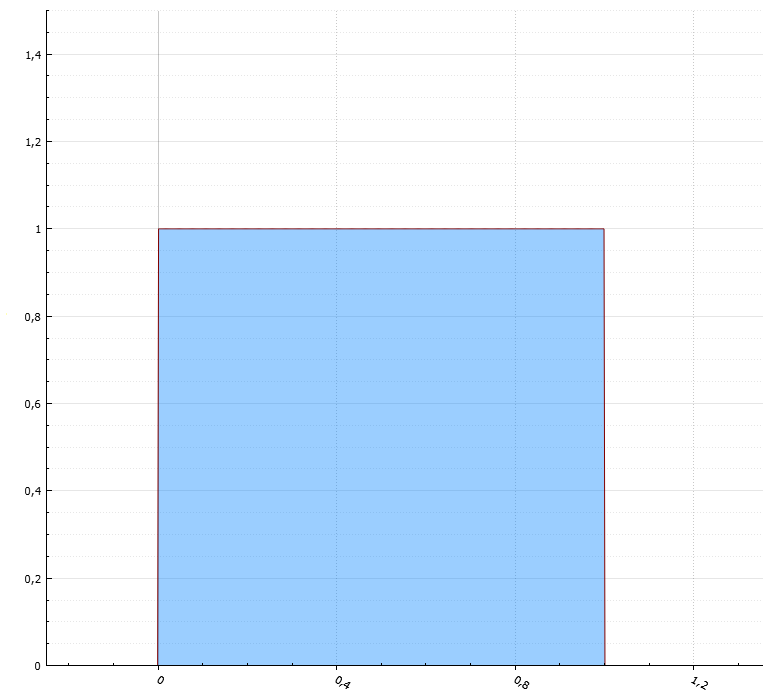
\includegraphics[width=\linewidth, right]{uniform}
						\captionsetup{labelformat=empty}
						\caption{$h(\vartheta)$}
					\end{minipage}
				\end{figure}
			
									
				\begin{figure}[!htb]\centering
					\begin{minipage}{0.7\textwidth}
						Апостериорная плотность вероятности:
						\[f(\vartheta \mid x) = \frac{\vartheta^x (1-\vartheta)^{n-x} 1_{(0,1)}(\vartheta)}{B(x+1, n-x+1)}, \]
						
						где в знаменателе бета-функция:
						\[B(a,b)=\int_{0}^{1} \vartheta^{a-1} (1-\vartheta)^{b-1} d \vartheta. \]
					\end{minipage}
					\begin{minipage}{0.18\textwidth}\centering
						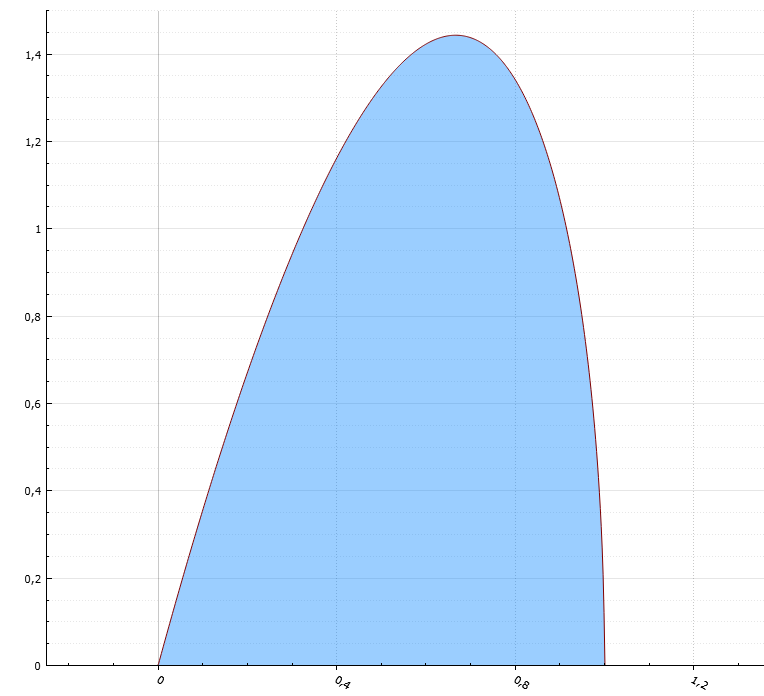
\includegraphics[width=\linewidth, height=2.6cm, right]{beta}
						\captionsetup{labelformat=empty}
						\caption{$f(\vartheta \mid x)$}
					\end{minipage}
				\end{figure}
			
			Тогда Байесовская оценка:
		\[g^*(x)=\ME[\theta|X=x]=\int_0^1 \frac{\vartheta^{x+1}(1-\vartheta^{n-x})}{B(x+1, n-x+1)}=\frac{B(x+2, n-x+1)}{B(x+1, n-x+1)} =\frac{x+1}{n+2},\]
		и Байесовский риск:
		\[
		\begin{aligned}
			R(\pi,g^*) & =\int_0^1 R(\vartheta, g^*) d\vartheta=\int_0^1 \ME_\vartheta\Big[\Big(\frac{X+1}{n+2}-\vartheta \Big)^2\Big]d\vartheta \\
			 & =\frac{1}{(n+2)^2} \int_0^1 (n\vartheta - n\vartheta^2+1-4\vartheta+4\vartheta^2)\ d\vartheta=\frac{1}{6(n+2)}.  
		\end{aligned}
		\]
	\end{itemize}
\end{exmp}

\begin{exmp}
	Пусть $X_1, \dots, X_n$ i.i.d. $\sim P_\mu^1=\mathcal{N}(\mu, \sigma^2)$ с заранее известным параметром $\sigma^2$. Априорное распределение $\mu$:
	\[ 
	h(\mu) = \frac{1}{\sqrt{2 \pi \tau^2}} \exp \Big\{ -\frac{(\mu-\mu_0)^2}{2\tau^2} \Big\}.
	\]
	Используя плотность распределения $X$
	\[
	f(x|\mu)=\Big( \frac{1}{\sqrt{2\pi \sigma^2}}\Big)^n \exp \Big\{ \frac{1}{2\sigma^2}\sum_{j=1}^n(x_j-\mu)^2 \Big \},
	\]
	получаем апостериорное распределение:
	\[  
	Q^{\mu|X=x} \sim \mathcal{N} \Big( g_{\mu_0, \tau^2}(x), \Big( \frac{n}{\sigma^2} + \frac{1}{\tau^2}\Big)^{-1}  \Big),
	\]
	где
	\[ 
	g_{\mu_0, \tau^2}(x)=\Big( 1 + \frac{\sigma^2}{n \tau^2} \Big)^{-1} \overline{x}_n+\Big( \frac{n \tau^2}{\sigma^2}+1 \Big)^{-1} \mu_0.
	\]
	Для квадратичного риска функция $g_{\mu_0, \tau^2}(x)$ -- Байесовская оценка. Интерпретация: при большом значении $\tau^2$ (мало априорной информации) оценка $g_{\mu_0, \tau^2}(x) \approx \overline{x}_n$, иначе $g_{\mu_0, \tau^2}(x) \approx \mu_0$.
\end{exmp}

\begin{defn}
	Пусть $g$ -- оценка $\gamma(\vartheta)$. Тогда:
	\[ R^*(g)=\sup_{\vartheta \in \Theta} R(\vartheta, g) \]
	называется \textbf{\textit{максимальным риском}} $g$ и
	\[ R^*(g^*)= \inf_{g \in \mathcal{K}} R^*(g) \]
	называется \textbf{\textit{минимаксным риском}}, а соответствующая оценка $g^*$ -- \textbf{\textit{минимаксной}}.
\end{defn}

\begin{rmrk} \
	\begin{enumerate}
		\item Использование минимаксной оценки нацелено на защиту от больших потерь.
		\item Пусть $\mathcal{M} = \{ \pi \mid \pi \text{ -- вероятностная мера на } \mathcal{A}_\Theta \}$. Тогда несложно заметить, что:
		\[ R^*(g)=\sup_{\pi \in \mathcal{M}} R(\pi, g). \]
	\end{enumerate}
\end{rmrk}

\begin{defn}
	Априорное распределение $\pi^*$ на $\mathcal{A}_\Theta$ называется \textbf{\textit{наименее благоприятным априорным}}, если
	\[ \inf_{g \in \mathcal{K}} R(\pi^*, g) \geq \inf_{g \in \mathcal{K}} R(\pi, g) \quad \forall \pi \in \mathcal{M}. \]
\end{defn}

\begin{thm} \
	\begin{enumerate}
		\item Если $g_\pi$ -- Байесовская оценка относительно $\pi$ и 
		\begin{equation} \label{eq3.2}
		 R(\pi, g_\pi) = \sup_{\vartheta \in \Theta} R(\vartheta, g_\pi),
		\end{equation}
		то $g_\pi$ -- минимаксная оценка.
		\item Если $g_\pi$ -- единственная Байесовская оценка относительно $\pi$, удовлетворяющая равенству \eqref{eq3.2}, то $g_\pi$ -- единственная минимаксная оценка.
		\item Если равенство \eqref{eq3.2} выполняется, то $\pi$ -- наименее благоприятное априорное распределение.
	\end{enumerate}
\end{thm}

\begin{proof} \
	\begin{enumerate}
		\item Для любой оценки $g \in \mathcal{K}$:
		\[ \sup_{\vartheta \in \Theta}R(\vartheta, g) \geq \int_{\Theta}R(\vartheta, g)\pi(d\vartheta) \geq \int_{\Theta}R(\vartheta, g_\pi)\pi(d\vartheta)=R(\pi, g_\pi)=\sup_{\vartheta \in \Theta}R(\vartheta, g_\pi). \]
		\item Если $g_\pi$ -- единственная Байесовская оценка для $\pi$, то
		\[ \int_{\Theta} R(\vartheta, g)\pi(d\vartheta) > \int_{\Theta} R(\vartheta, g_\pi)\pi(d\vartheta) \quad \forall g \neq g_\pi. \]
		Тогда $\sup_{\vartheta \in \Theta}R(\vartheta, g) > \sup_{\vartheta \in \Theta}R(\vartheta, g_\pi) $ и $g_\pi$ единственная минимаксная оценка.
		\item Для любого распределения $\mu \in \mathcal{M}$:
		\[ \inf_{g \in \mathcal{K}} \int_{\Theta} R(\vartheta, g)\mu(d\vartheta) \leq \int_{\Theta}R(\vartheta, g_\pi)\mu(d\vartheta) \leq \sup_{\vartheta \in \Theta} R(\vartheta, g_\pi) = R(\pi, g_\pi) = \inf_{g \in \mathcal{K}} \int_{\Theta}R(\vartheta, g) \pi(d\vartheta). \]
	\end{enumerate}
\end{proof}

\begin{rmrk}
	Иногда функция риска Байесовской оценки $g_\pi$ является постоянной:
	\[ R(\vartheta, g_\pi) = c \quad \forall \vartheta \in \Theta. \]
	Тогда
	\[ \sup_{\vartheta \in \Theta} R(\vartheta, g_\pi) = c = \int_{\Theta} R(\vartheta, g_\pi) \pi(d\vartheta) = R(\pi, g_\pi), \]
	равенство \eqref{eq3.2} выполняется, $g_\pi$ минимаксная оценка и $\pi$ -- наименее благоприятное априорное распределение.
\end{rmrk}

\begin{exmp} \label{exmp3.14}
	Пусть $\Theta = (0, 1)$, $\mathcal{X}=\{0, \dots, n \}$ и 
	\[ P_\vartheta(X = x) = \binom{n}{x} \vartheta^x (1-\vartheta)^{n-x}. \]
	Мы снова используем квадратичный риск и выбираем бета-распределение в качестве априорного:
	\[ h(\vartheta) = \frac{\vartheta^{a-1}(1-\vartheta)^{b-1}1_{[0,1]}(\vartheta)}{B(a, b)}. \]
	Апостериорное распределение $Q^{\vartheta|X=x} \sim B(x+a,n-x+b)$ с плотностью:
	\[ f(\vartheta | x)= \frac{\vartheta^{x+a-1}(1-\vartheta)^{n-x+b-1}1_{[0,1](\vartheta)}}{B(x+a,n-x+b)}.  \]
	Несложно доказать, что для случайной величины $Z$ с бета-распределением $B(p,q)$
	\[\ME[Z]=\frac{p}{p+q} \quad \text{и} \quad \Var(Z)=\frac{pq}{(p+q)^2(p+q+1)}.	\]
	Используя Теорему \ref{thm3.5}, получаем Байесовскую оценку для $\vartheta$:
	\[g_{a,b}(x)=\frac{x+a}{n+a+b}. \]
	Соответствующий ей риск:
	\[ R(\vartheta, g_{a,b})=\ME[(g_{a,b}(X)-\vartheta)^2]=\frac{\vartheta^2(-n+(a+b)^2+\vartheta(n-2a(a+b))+a^2}{(n+a+b)^2}. \]
	Если выбрать постоянные $a^*=b^*=\sqrt{n}/2$, то риск будет равен:
	\[ R(\vartheta, g_{a^*,b^*})=\frac{1}{4(\sqrt{n} + 1)^2}. \]
	Такой риск не зависит от $\vartheta$, а значит оценка
	$g_{a^*,b^*}(x) = \frac{x+\sqrt{n}/2}{n+\sqrt{n}}$
	является минимаксной и $B(a^*, b^*)$ -- наименее благоприятное распределение.	
\end{exmp}


\begin{defn}
	Пусть
	\[ r_\pi = \inf_{g \in \mathcal{K}}R(\pi, g), \quad \pi \in \mathcal{M}. \]
	Последовательность $(\pi_m)_{m \in \MN}$ в $\mathcal{M}$ называется \textbf{\textit{наименее благоприятной последовательностью априорных распределений}}, если
	\begin{enumerate}
		\item $\lim\limits_{m \rightarrow \infty} r_{\pi_m}=r,$
		\item $ \forall \pi \in \mathcal{M} \quad r_\pi \leq r.$
	\end{enumerate}
\end{defn}

\begin{thm} \label{thm3.16}
	Пусть $(\pi_m)$ в $\mathcal{M}$ последовательность, такая что  $r_{\pi_m} \rightarrow r \in \MR$. Также пусть существует такая оценка $g^* \in \mathcal{K}$, что:
	\[ \sup_{\vartheta \in \Theta} R(\vartheta, g^*) = r. \]
	Тогда:
	\begin{enumerate}
		\item $g^*$ -- минимаксная оценка,
		\item $(\pi_m)$ -- наименее благоприятная последовательность априорных распределений.
	\end{enumerate}
\end{thm}

\begin{proof} \
	\begin{enumerate}
		\item Для любой оценки $g \in \mathcal{K}$
		\[ \sup_{\vartheta \in \Theta} R(\vartheta, g) \geq \int_{\Theta}R(\vartheta, g)\pi_m(d\vartheta) \geq r_{\pi_m} \longrightarrow r=\sup_{\vartheta \in \Theta}R(\vartheta, g^*). \]
		\item Для любого распределения $\pi \in \mathcal{M}$
		\[ r_\pi \leq R(\pi, g^*)=\int_{\Theta} R(\vartheta, g^*) \pi(d \vartheta) \leq \sup_{\vartheta \in \Theta}R(\vartheta, g^*)=r. \]
	\end{enumerate}
\end{proof}

\begin{exmp}
	Пусть $X_1, \dots, X_n$ i.i.d. $\sim \mathcal{N}(\mu, \sigma^2)$ с известным параметром $\sigma^2$. В качестве априорного распределения выбираем:
	\[ h_m(\mu)=\frac{1}{\sqrt{2 \pi m}} \exp \Big \{ -\frac{(\mu-\mu_0)^2}{2m}\Big \}. \]
	Байесовская оценка:
	\[ g_m(x)=\Big( 1 + \frac{\sigma^2}{n m} \Big)^{-1} \overline{x}_n+\Big( \frac{n m}{\sigma^2}+1 \Big)^{-1} \mu_0.\]
	Для любого значения $\mu \in \MR$:
	\[  
	\begin{aligned}
	R(\mu, g_m) & = \ME_\mu[(g_m(X)-\mu)^2] \\
	& = \ME_\mu\Bigg[\bigg(\Big( 1 + \frac{\sigma^2}{n m} \Big)^{-1} (\overline{X}_n-\mu)+\Big( \frac{n m}{\sigma^2}+1 \Big)^{-1} (\mu_0-\mu)\bigg)^2\Bigg] \\
	& = \Big(1 + \frac{\sigma^2}{nm}\Big)^{-2} \frac{\sigma^2}{n} + \Big( 1+\frac{nm}{\sigma^2} \Big)^{-2}(\mu_0-\mu)^2 \xrightarrow[m \ \rightarrow \infty]{} \frac{\sigma^2}{n}
	\end{aligned}
	\]
	Так как риск ограничен сверху:
	\[ R(\mu, g_m) \leq \frac{\sigma^2}{n} + (\mu - \mu_0)^2, \]
	то по теореме Лебега о мажорируемой сходимости\footnote{
		Пусть фиксировано измеримое пространство $(X, \mathcal{F}, \mu)$. Предположим, что $\{ f_n \}_{n=1}^\infty$ и $f$ -- измеримые функции на $X$, причем $f_n(x) \rightarrow f(x)$ почти всюду. Тогда если существует определённая на том же пространстве интегрируемая функция $g$, такая что
		\[ |f_n(x)| \leq g(x) \quad \forall n \in \MN \]
		почти всюду, то $f_n$ и $f$ интегрируемы и
		\[ \lim\limits_{n \rightarrow \infty} \int_X f_n(x) \mu(dx) = \int_X f(x) \mu(dx). \]
		}:
	\[ r_{\pi_m}=R(\pi_m, g_m)=\int_{\MR}R(\mu, g_m)\pi_m(d\mu) \longrightarrow \frac{\sigma^2}{n}. \]
	Очевидно, $g^*(x)=\overline{x}_n$ удовлетворяет равенству
	\[ R(\mu, g^*)=\ME_\mu[(\overline{X}_n-\mu)^2]=\frac{\sigma^2}{n}, \]
	следовательно по Теореме \ref{thm3.16} $g^*$ -- минимаксная оценка и $\pi_m$ -- наименее благоприятная последовательность априорных распределений.
\end{exmp}

\raggedbottom
\pagebreak

\section*{Упражнения}
\begin{exc}
	Пусть $X \sim Po(\lambda)$ (распределение Пуассона). Функция потерь:
	\[ L(\lambda, a) = (\lambda - a)^2/\lambda. \]
	Докажите, что оценка $g(X)=X$ является минимаксной для параметра $\lambda$. Используйте следующие шаги:
	\begin{enumerate}
		\item Выберите гамма-распределение $\pi_{\alpha, \beta}=\Gamma(\alpha, \beta)$ в качестве априорного. Найдите апостериорное распределение.
		\item Рассчитайте апостериорный риск:
		\[ R_{\pi_{\alpha, \beta}}^x(a) := \int_{\Theta} L(\lambda, a) Q^{\lambda | X = x} (d\lambda). \]
		для $a \in \MR$ и $\alpha>1$. \\
		\subitem \textit{\textit{Подсказка}:} если $\Lambda \sim \Gamma(\alpha, \beta)$, то 
		\[ \ME[\Lambda]=\frac{\alpha}{\beta}, \quad \ME[1/\Lambda]=\frac{\beta}{\alpha-1}. \]
		\item Найдите значение $a^*$, доставляющее минимум апостериорному риску $R_{\pi_{\alpha, \beta}}^x(a)$. Рассчитайте соответствующий минимум $R_{\pi_{\alpha, \beta}}^x(a^*)$.
		\item Рассчитайте $R(\lambda, X)$ и тем самым завершите доказательство.
	\end{enumerate}
\end{exc}

\begin{exc}
	Докажите следующие утверждения:
	\begin{enumerate}
		\item Если $g^*$ -- допустимая оценка с постоянным риском, то $g^*$ -- минимаксная.
		\item Если $g^*$ -- Байесовская оценка для априорного распределения $\pi$ и единственная в том смысле, что для любой другой Байесовской оценки $\tilde{g}$
		\[ R(\vartheta, g^*)=R(\vartheta, \tilde{g}) \quad \forall \vartheta \in \Theta, \]
		то $g^*$ -- допустимая.
	\end{enumerate}
\end{exc}

\begin{exc}
	Пусть $X_1, \dots, X_n$ i.i.d. $\sim \mathcal{N}(\mu, \sigma^2)$, $X=(X_1, \dots, X_n)^T$ и функция потерь:
	\[ L(\sigma^2,d)=(d/\sigma^2-1)^2. \]
	Предположим, что $\mu=0$. Докажите, что
	\[ g(X)=\frac{1}{n+2}\sum_{i=1}^{n}X_i^2 \]
	является минимаксной оценкой $\sigma^2$. \\
	\subitem \textit{Подсказка}: произведите замену $\lambda=1/\sigma^2$ и возьмите для этого параметра априорное распределение $\pi_{\alpha, \beta}=\Gamma(p, b)$. Заметьте, что для апостериорного риска $g$:
	\[R_{\pi_{\alpha, \beta}}^x(\sigma^2, g)=\int_{\Theta}L(\sigma^2, g(x))Q^{\theta|X=x}d(1/\sigma^2)=\int_{\Theta}(g(x)\lambda-1)^2Q^{\theta|X=x}d(\lambda).\]
\end{exc}
\chapter{Достаточность и полнота}

Теперь, пусть $(\mathcal{X}, \mathcal{B}, P)$, где $P \in \mathcal{P} = \{P_\vartheta \mid \vartheta \in \Theta \} $, -- вероятностное пространство и $(\mathcal{T}, \mathcal{D})$ -- измеримое пространство.

\begin{defn}
	$\mathcal{B}$-$\mathcal{D}$-измеримая функция $T:\mathcal{X} \rightarrow \mathcal{T}$ называется \textbf{\textit{статистикой}}.
\end{defn}

\begin{exmp} \label{exmp4.2}
	Пусть $X_1, \dots, X_n$ i.i.d. $\sim \mathrm{Bin}(1, \vartheta)$ с совместным распределением:
	\[ f(x, \vartheta) = \vartheta^{\sum_{i=1}^{n}x_i}(1-\vartheta)^{n-\sum_{i=1}^{n}x_i}=\vartheta^{T(x)}(1-\vartheta)^{n-T(x)}, \]
	где $T(x)=\sum_{i=1}^{n}x_i$ -- статистика.
	Если мы выбираем $u_1, \dots, u_n \in \{0,1\}$, то
	\[
		P_\vartheta(X_i=u_i \  \forall i = 1, \dots, n \mid T(X)=k)=\left \{
		\begin{array}{cl}
		\frac{1}{\binom{n}{k}}, & \text{если } \sum_{i=1}^{n}u_i=k \\
		0, & \text{иначе}
		\end{array}
		\right.
	\]
	Мы видим, что в данном примере, зная значение $T(X)$, никакой дополнительной информации о $\vartheta$ не может быть получено из информации о векторе $X=X_1, \dots, X_n$.
\end{exmp}

\begin{defn} \
	\begin{enumerate}
		\item $\sigma$-алгебра $\mathcal{C} \subset \mathcal{B}$ называется \textbf{\textit{достаточной}} для $\vartheta$, если
		\[ k_B=P_\vartheta(B | \mathcal{C}) \quad \forall \vartheta \in \Theta,\ \forall B \in \mathcal{B}. \]
		Это означает, что $\mathcal{C}$-условные вероятности не зависят от $\vartheta$.
		\item Статистика $T\colon\mathcal{X} \rightarrow \mathcal{T}$ называется \textbf{\textit{достаточной}} для $\vartheta$, если $\sigma(T)$ достаточна для $\vartheta$.
	\end{enumerate}
\end{defn}

\begin{rmrk} \
	\begin{enumerate}
		\item Из Леммы о факторизации (Теорема \ref{Factorization lemma}) мы знаем, что $T$ достаточная для $\vartheta$ тогда и только тогда, когда $\forall B \in \mathcal{B}$ существует функция $h_B\colon\mathcal{T} \rightarrow \MR$, такая что:
		\[ h_B(t)=P_\vartheta(B \mid T=t). \]
		\item В Примере \ref{exmp4.2} статистика $T(x)=\sum_{i=1}^{n}x_i$ достаточная для $\vartheta$.
		\item Пусть $g\colon\mathcal{X} \rightarrow \MR$ из $L^1(\mathcal{P}) = \bigcap_{\vartheta \in \Theta}L^1(P_\vartheta)$.
		\begin{enumerate}
			\item Если $\mathcal{C}$ достаточная для $\vartheta$, то существует функция
			\[ k = \ME_\vartheta[g | \mathcal{C}], \]
			не зависящая от $\vartheta$.
			\item Если $T\colon \mathcal{X} \rightarrow \mathcal{T}$ достаточная для $\vartheta$, то существует функция
			\[h(t)=\ME_\vartheta[g \mid T=t],\]
			не зависящая от $\vartheta$.
		\end{enumerate}
	\end{enumerate}
\end{rmrk}

\begin{exmp}
	Пусть $Q$ -- конечная группа отображений $\pi\colon (\mathcal{X}, \mathcal{B}) \rightarrow (\mathcal{X}, \mathcal{B})$. Система
	\[ \mathcal{C}=\mathcal{C}(Q)=\{ B \in \mathcal{B} \mid \pi(B)=B \ \ \forall \pi \in Q \} \]
	называется $\sigma$-алгеброй $Q$-инвариантных множеств. Если $\mathcal{P}$ инвариантна относительно $Q$, то есть:
	\[P_\vartheta^\pi(B)=P_\vartheta(\pi^{-1}(B))=P_\vartheta(B) \quad \forall B \in \mathcal{B},\ \forall \pi \in Q,\ \forall \vartheta \in \Theta\]
	и если $g \in L^1(\mathcal{P})$ и $q=|Q|$, то
	\[ k(x)=\frac{1}{q} \sum_{\pi \in Q} g(\pi(x)) \]
	является версией $\ME_\vartheta[g|\mathcal{C}]$, независимой от $\vartheta$. Как следствие, $\mathcal{C}$ -- достаточная.
\end{exmp}
\begin{proof}
	Так как $Q$ является группой, то $k(x)=k(\pi(x)) \ \forall \pi \in Q$. Следовательно, 
	\[ k^{-1}(B)=(\pi)^{-1}(k^{-1}(B)) \quad \forall B \in \mathcal{B}, \]
	иными словами, $k$ -- $\mathcal{C}$-измерима. Пусть $C \in \mathcal{C}$, тогда:
	\[
	\begin{aligned}
	    \int_{C} k(x)P_\vartheta(dx) & =\frac{1}{q}\sum_{\pi \in Q} \int_{C} g(\pi(x)) P_\vartheta(dx)=\frac{1}{q}\sum_{\pi \in Q} \int_{\pi(C)} g(x) P_\vartheta^\pi(dx) \\
	    & = \frac{1}{q}\sum_{\pi \in Q} \int_{\pi(C)} g(x) P_\vartheta(dx) = \frac{1}{q}\sum_{\pi \in Q} \int_{C} g(x) P_\vartheta(dx)\\
	    & = \int_{C} g(x)P_\vartheta(dx).
	\end{aligned}
	 \]
\end{proof}

\begin{exmp}
	Пусть $X_1, \dots, X_n$ i.i.d. $\sim F$ и 
	\[ \mathcal{P}= \{ P \sim F^n \mid F \text{ -- функция распределения} \}, \quad F^n(x)=\prod_{i=1}^{n}F(x_i). \]
	Также $\mathcal{X}=\mathbb{P}^n$ и $\mathcal{B}=\mathcal{B}^n$. Пусть
	\[ Q=S_n=\{ \pi\colon\MR^n \rightarrow \MR^n \mid \pi \text{ -- перестановка} \}, \]
	тогда $P^\pi = P  \quad \forall \pi \in S_n $ и таким образом $\mathcal{P}$ -- инвариантна относительно $S_n$. Следовательно, $\mathcal{C}=\mathcal{C}(S_n)$ -- достаточная.
\end{exmp}

\begin{defn}
	Пусть $\MR_{\leq}^n = \{X \in \MR^n | X_1 \leq \dots \leq X_n \}$ и $X_{(j)}$ -- $j$-ое наименьшое число среди $X_1, \dots, X_n$. Тогда статистика
	\[T\colon
	\left \{
	\begin{array}{ccl}
	\MR^n & \rightarrow & \MR_{\leq}^n \\
	X & \mapsto & X_{(\cdot)}
	\end{array}
	\right.
	 \]
	называется \textbf{\textit{порядковой статистикой}} $(X_1, \dots, X_n)^T$. 
\end{defn}

\begin{rmrk} \label{rmrk4.8} \
	\begin{enumerate}
		\item По определению $\sigma(T) = \mathcal{C}(S_n)$, поэтому $T$ -- достаточная статистика. Другими словами, всегда достаточно хранить упорядоченный вектор наблюдений.
		\item Статистика
		\[\widetilde T\colon
		\left \{
		\begin{array}{ccl}
		\MR^n & \rightarrow & \MR^n \\
		X & \mapsto & \big(\sum_{i=1}^n X_i, \sum_{i=1}^{n}X_i^2, \dots, \sum_{i=1}^{n}X_i^n\big)^T
		\end{array}
		\right.
		\]
		также достаточная, потому что можно показать, что $\sigma(T)=\sigma(\widetilde T)$.
	\end{enumerate}
\end{rmrk}

\begin{defn}
	Пусть $\mathcal{P}= \{ P_\vartheta \mid \vartheta \in \Theta \}$ -- семейство вероятностных мер. Тогда мера $\nu$ называется \textbf{\textit{эквивалентной}} $\mathcal{P}$, если
	\[ \nu(N) = 0 \Longleftrightarrow P_\vartheta(N)=0 \quad \forall \vartheta \in \Theta. \]
\end{defn}

\begin{thm}[\textbf{Теорема Халмоса-Саважа}] \label{Halmos-Savage}
	Пусть $\mu$ -- $\sigma$-конечная мера, $\mathcal{P}=\{P_\vartheta \mid \vartheta \in \Theta \}$ и $P_\vartheta \ll \mu \quad \forall \vartheta \in \Theta $.
	\begin{enumerate}
		\item Существует мера $\nu$, эквивалентная $\mathcal{P}$, вида
		\begin{equation} \label{eq4.1}
		\nu = \sum_{i=1}^{\infty}c_iP_{\vartheta_i},\; \text{где } c_i \geq 0 \; \forall i \text{ и } \sum_{i=1}^{\infty}c_i=1.
		\end{equation}
		\item $\sigma$-алгебра $\mathcal{C} \subset \mathcal{B}$ достаточная для $\vartheta$ тогда и только тогда, когда существует $\mathcal{C}$-измеримая функция $\frac{dP_\vartheta}{d\nu}$ для любого параметра $\vartheta$.
		\item Статистика $T$ является достаточной для $\vartheta$ тогда и только тогда, когда для любого параметра $\vartheta$ существует  функция $g_\vartheta$, такая что:
		\[ \frac{dP_\vartheta}{d\nu}(x)=g_\vartheta(T(x)). \]
	\end{enumerate}
\end{thm}
\begin{proof} \
	\begin{enumerate}
		\item Мы докажем утверждение только для конечной меры $\mu$. Пусть
		\[ \mathcal{J} = \{\nu\ |\ \nu \text{ -- мера вида \eqref{eq4.1}}  \} \]
		и
		\[ q = \frac{dQ}{d\mu}, \quad Q \in \mathcal{J}. \]
		Достаточно показать, что существует мера $Q_0 \in \mathcal{J}$, такая что:
		\begin{equation} \label{eq4.2}
		Q_0(A) = 0 \Longrightarrow Q(A) = 0 \quad \forall Q \in \mathcal{J}.
		\end{equation}
		Тогда $P_\vartheta(A) = 0$ $\forall \vartheta$, так как $P_\vartheta \in \mathcal{J}$. Верно и обратное, если $P_\vartheta(A) = 0$ $\forall \vartheta$, то $Q_0(A) = 0$, так как $Q_0 \in \mathcal{J}$. Рассмотрим множество
		\[ \mathcal{C}:= \{ B \in \mathcal{B}\ |\ \exists Q \in \mathcal{J}  \text{, такая что } Q(B) > 0 \text{ и } q(x) > 0 \text{ для $\mu$-почти всех }  x \in B \} \]
		и зададим $\sup_{B \in \mathcal{C}} \mu(B) = r$. Тогда существуют $B_i \in \mathcal{C}$, такие что $\mu(B_i) \rightarrow r$. Пусть 
		\[B_0 = \bigcup_{i \in \MN}B_i,\]
		тогда вследствие непрерывности $\mu$ мы получаем $\mu(B_0)=r$. Пусть также $Q_i$ -- меры $Q\in\mathcal{J}$, соответствующие $B_i$, и
		\[ Q_0 = \sum_{i=1}^{n} c_i Q_i \in \mathcal{J}, \]
		где $c_i > 0$ и $\sum_{i=1}^{n} c_i = 1$. Тогда $\mu$-плотность $Q_0$:
		\[ \frac{dQ_0}{d\mu}(x) = q_0(x) = \sum_{i=1}^{n} c_i q_i(x). \]
		Очевидно, что $q_0(x) > 0$ для $\mu$-почти всех $x \in B_0$. Следовательно $Q_0(B_0) > 0$ и $B_0 \in \mathcal{C}$. Докажем \eqref{eq4.2}. Допустим, $Q_0(A) = 0$ и пусть $Q \in \mathcal{J}$ -- произвольная мера. Пусть $q$ -- плотность $Q$ и
		\[ B = \{x\ |\ q(x) > 0  \}. \]
		Тогда
		\[0 = Q_0(A \cap B_0 ) = \int_{A \cap B_0} q_0(x) \mu(dx).\]
		Так как на $q_0 > 0$ на $B_0$, мы получаем
		\[ \mu(A \cap B_0) = 0 \]
		и, как следствие,
		\[ Q(A \cap B_0) = 0 \quad \forall Q \in \mathcal{J}. \]
		Кроме того, в соответствии с определением $B$:
		\[ Q(A \cap B_0^c \cap B^c ) = 0.\]
		Если $Q(A \cap B_0^c \cap B ) > 0$, то $B_0$ и $A \cap B_0^c \cap B$ являются элементами $\mathcal{C}$. Тогда легко увидеть, что объединение $B_0$ и $A \cap B_0^c \cap B$ также принадлежит $\mathcal{C}$. Тогда
		\[ \mu(B_0 \cup (A \cap B_0^c \cap B)) = \mu(B_0) + \mu(A \cap B_0^c \cap B) > \mu(B_0), \]
		что противоречит максимальности $B_0$ в $\mathcal{C}$. Следовательно,
		\[ Q(A \cap B_0^c \cap B ) = 0 \Longrightarrow Q(A) = 0. \]
		\item ''$\Longrightarrow$'' Допустим, что $\mathcal{C}$ -- достаточная. Тогда $\forall B \in \mathcal{B}$ существует $\mathcal{C}$-измеримая функция $k_B$, независимая от $\vartheta$, такая что
		\[ \int_C k_B dP_\vartheta = \int_C 1_B dP_\vartheta \quad \forall C \in \mathcal{C}\ \forall \vartheta \in \Theta. \]
		Из (i) следует, что
		\[ \int_C k_B d\nu = \int_C 1_B d\nu \quad \forall C \in \mathcal{C}. \]
		Следовательно, $k_B = \ME_\nu[1_B|\mathcal{C}]$ и
		\[ P_\vartheta(B) = \int_{\mathcal{X}} 1_B dP_\vartheta = \int_{\mathcal{X}} k_B dP_\vartheta = \int_{\mathcal{X}} \ME_\nu[1_B|\mathcal{C}]dP_\vartheta. \]
		Пусть теперь 
		\[f_\vartheta^\mathcal{C} = \frac{dP_\vartheta^\mathcal{C}}{d \nu}\]
		-- $\nu$-плотность $P_\vartheta$, ограниченная $\sigma$-алгеброй $\mathcal{C}$. Тогда вследствие $\mathcal{C}$-измеримости $f_\vartheta^C$ (Теорема \ref{Radon Nikodym}) мы получаем по Теореме \ref{Factorization theorem}:
		\[ P_\vartheta(B) = \int_{\mathcal{X}} \ME_\nu[1_B | \mathcal{C}]f_\vartheta^{\mathcal{C}} d\nu = \int_{\mathcal{X}}\ME_\nu[1_B f_\vartheta^\mathcal{C} | \mathcal{C} ] d\nu = \int_B f_\vartheta^\mathcal{C} d\nu. \]
		Следовательно, $\frac{dP_\vartheta}{d \nu} = f_\vartheta^\mathcal{C}$ и $f_\vartheta^\mathcal{C}$ $\mathcal{C}$-измерима.\\
		
		''$\Longleftarrow$'' Пусть $B \in \mathcal{B}$ и $k_B$ -- версия $\ME_\nu[1_B|\mathcal{C}]$, где $\nu$ -- мера из (i). Тогда для $f_\vartheta = \frac{dP_\vartheta}{d\nu}$ имеет место
		\[ \int_C 1_B dP_\vartheta = \int_{B \cap C} f_\vartheta d\nu = \int_C 1_B f_\vartheta d\nu = \int_C \ME_\nu[1_B f_\vartheta | \mathcal{C}]d\nu \quad \forall C \in \mathcal{C}. \]
		$f_\vartheta$ $\mathcal{C}$-измерима по предположению. Таким образом,
		\[ \int_C 1_B dP_\vartheta = \int_C f_\vartheta \ME_\nu[1_B | \mathcal{C}]d\nu = \int_C f_\vartheta k_B d\nu = \int_C k_B dP_\vartheta \]
		и $\mathcal{C}$ -- достаточная по определению.
		\item Следует из (ii) и Леммы о факторизации (Теорема \ref{Factorization lemma}).
    \end{enumerate}
\end{proof}

\begin{thm}[\textbf{Критерий Неймана}] \label{Neyman criterion} Пусть $\mu$ -- $\sigma$-конечная мера и $P \ll \mu$. Тогда:
	\begin{enumerate}
		\item $\sigma$-алгебра $\mathcal{C}$ является достаточной для $\vartheta \in \Theta$ тогда и только тогда, когда существуют $\mathcal{C}$-измеримые функции $f_\vartheta\colon\mathcal{X} \rightarrow \MR$ и $\mathcal{B}$-измеримая функция $r:\mathcal{X} \rightarrow \MR$, такие что
		\[ \frac{dP_\vartheta}{d\mu}=r(x)f_\vartheta(x). \]
		\item Статистика $T\colon(\mathcal{X},\mathcal{B}) \rightarrow (\mathcal{T},\mathcal{D})$ является достаточной тогда и только тогда, когда существуют $\mathcal{D}$-измеримые функции $g_\vartheta\colon\mathcal{T} \rightarrow \MR$ и $\mathcal{B}$-измеримая функция $r\colon\mathcal{X} \rightarrow \MR$, такие что
		\[\frac{dP_\vartheta}{d\mu}=r(x)g_\vartheta(T(x)). \]
	\end{enumerate}
\end{thm}
\begin{proof}
	Мы покажем только (i), так как (ii) следует из \ref{Factorization lemma}. \\
	''$\Longrightarrow$'' Пусть $r$ -- мера из Теоремы \ref{Halmos-Savage}, $P_\vartheta \ll r \ll \mu$. Из Теоремы \ref{Radon Nikodym} следует:
	\[
	\begin{aligned}
	\frac{dP_\vartheta}{d \mu}(x) = & \underbrace{\frac{d P_\vartheta}{d \nu}(x)} & \underbrace{\frac{d \nu}{d \mu}(x)} \\
    &\ f_\vartheta(x) & r(x) \
	\end{aligned} \] 
	$f_\vartheta(x)$ $\mathcal{C}$-измерима по Теореме \ref{Halmos-Savage}(ii). \\
	''$\Longleftarrow$''
	$f_\vartheta(x)$ $\mathcal{C}$-измерима по предположению. Возьмем $c_i$ и $f_{\vartheta_i}$ из $r$ из Теоремы \ref{Halmos-Savage} и определим:
	\[ \widetilde{f_\vartheta}(x) =
	\left \{
	\begin{array}{cl}
	f_\vartheta(x) / \sum_{i=1}^{\infty} c_i f_{\vartheta_i}(x) , & \exists\ i: f_{\vartheta_i}(x) > 0, \\
	0, & \text{иначе}.
	\end{array}
	\right.
	\]
	Следовательно, $\widetilde{f_\vartheta}$ $\mathcal{C}$-измерима и
	\[ \int_B  \widetilde{f_\vartheta}d\nu = \int_B \widetilde{f_\vartheta} \sum_{i=1}^{\infty} c_i dP_{\vartheta_i} = \int_B \widetilde{f_\vartheta} \sum_{i=1}^{\infty} c_i r f_{\vartheta_i}d\mu = \int_B f_\vartheta r d\mu \quad \forall B \in \mathcal{B},  \]
	что не что иное, как $P_\vartheta(B)$. Следовательно, $\widetilde{f_\vartheta}$ $\mathcal{C}$-измеримая версия $\frac{dP_\vartheta}{dr}$. Следовательно, по Теореме \ref{Halmos-Savage} (ii) $\mathcal{C}$ достаточная для $\vartheta$.
\end{proof}

\begin{exmp} \label{exmp4.12} \
	\begin{enumerate}
		\item Пусть $P$ -- $k$-параметрическое экспоненциальное семейство с плотностями
		\[ \frac{dP_\vartheta}{d \mu}(x) = c(\vartheta)h(x)\exp\Big\{\sum_{i=1}^k Q_j(\vartheta)T_j(x)\Big \}. \]
		По Теореме \ref{Neyman criterion} $T = (T_1, \dots, T_n)^T$ достаточная для $\vartheta$.
		\item Если $X_i \sim \mathcal{N}(\mu, \sigma^2)$, то
		\[ T(X) = \Big(\sum_{i=1}^{n}X_i, \sum_{i = 1}^{n} X_i^2 \Big) \]
		достаточная для $(\mu, \sigma^2)^T$.
		\item Если $X_1, \dots, X_n$ i.i.d. $\sim \mathcal{U}[0, \vartheta]$ ($\vartheta > 0$), то для $X$ плотность вероятности будет:
		\[ f_\vartheta(X) = \bigg(\frac{1}{\vartheta} \bigg)^n \prod_{i = 1}^{n} 1_{[0, \vartheta]}(X_i) = \bigg(\frac{1}{\vartheta} \bigg)^n 1_{[0, \vartheta]} \big(\max_{1 \leq i \leq n} X_i \big). \]
		Следовательно, $T(X) = \max_{1 \leq i \leq n} X_i$ достаточная для $\vartheta$ по Теореме \ref{Neyman criterion}.
	\end{enumerate}
\end{exmp}

\begin{rmrk}\label{rmrk4.13}
	Пусть $T\colon(\mathcal{X}, \mathcal{B}) \rightarrow (\mathcal{T}, \mathcal{D})$ и $\widetilde{T}\colon(\mathcal{X}, \mathcal{B}) \rightarrow (\widetilde{\mathcal{T}}, \widetilde{\mathcal{D}})$ -- статистики и, без ограничения общности, $\mathcal{T} = T(\mathcal{X})$ и $\widetilde{\mathcal{T}}=\widetilde{T}(\mathcal{X})$. Если $T$ -- достаточная для $\vartheta$ и существует биекция $b\colon\mathcal{T} \rightarrow \widetilde{\mathcal{T}}$, такая что $\widetilde{T} = b \circ T$ и $b(\mathcal{D}) = \widetilde{\mathcal{D}}$, то
	\[ \widetilde{T}^{-1}(\widetilde{D}) = T^{-1}(b^{-1}(b(D))) = T^{-1}(D), \quad \widetilde{D} \in \widetilde{\mathcal{D}} \quad \text{и} \quad D = b^{-1}(\widetilde{D}) \in \mathcal{D}. \]
	Следовательно, $\sigma(\widetilde{T}) = \sigma(T)$ и $\widetilde{T}$ -- достаточная. \\
	Вкратце: биективное отображение сохраняет достаточность.
\end{rmrk}

\begin{exmp}
	Пусть $X_1, \dots, X_n$ i.i.d. $\sim \mathcal{N}(\mu, \sigma^2)$. Мы знаем из Примера \ref{exmp4.12}, что 
	\[ T(X) = \Big(\sum_{i=1}^{n}X_i, \sum_{i = 1}^{n} X_i^2 \Big) \]
	достаточная для $(\mu, \sigma^2)^T$. Из Замечания \ref{rmrk4.13} следует, что $(\overline{X}_n, \hat{s}_n^2)$ достаточная, если взять
	\[ b(x, y) = \bigg( \frac{x}{n}, \frac{y}{n}-\bigg(\frac{x}{n}\bigg)^2 \bigg), \quad \mathcal{T} = \bigg\{ (x, y) | x \in \MR, y \geq \frac{x^2}{n}\bigg \} \quad \text{и} \quad \widetilde{\mathcal{T}}=\MR \times \MR^+.
	 \]
	 Множество $\mathcal{T}$ может быть проверено с помощью неравенства Коши-Шварца.
\end{exmp}

\begin{thm}[\textbf{Теорема Рао-Блэквелла}] \label{Rao-Blackwell}
	Пусть $\mathcal{P}=\{P_\vartheta \mid \vartheta \in \Theta \}$ -- семейство распределений на $(\mathcal{X}, \mathcal{B})$, $T\colon(\mathcal{X}, \mathcal{B}) \rightarrow (\mathcal{T}, \mathcal{D})$ -- достаточная статистика для $\vartheta$, $\gamma \colon \Theta \rightarrow \Gamma \subset \MR^l$, $L\colon \Gamma \times \Gamma \rightarrow \MR^+$ -- функция потерь, такая что $y \mapsto L(\gamma(\vartheta), y)$ -- выпуклая $\forall \vartheta \in \Theta$. Если $g$ -- несмещенная оценка $\gamma(\vartheta)$ и $\ME[L(\gamma(\vartheta), g)] < \infty \ \forall \vartheta \in \Theta$, то:
	\begin{enumerate}
		\item Существует $\sigma(T)$-измеримая несмещенная оценка $k$, такая что
		\[ R(\vartheta, k) \leq R(\vartheta, g) \quad \forall \vartheta \in \Theta, \]
		точнее $k=\ME[g|T]$.
		\item Если $y \mapsto L(\gamma(\vartheta), y)$ строго выпуклая $\forall \vartheta \in \Theta$, то 
		\[ R(\vartheta, k) = R(\vartheta, g) \quad \forall \vartheta \in \Theta, \]
		тогда и только тогда, когда $g = h \circ T $, где $h(t)=\ME[g|T=t]$.
	\end{enumerate}
\end{thm}
\begin{proof}
	Используем неравенство Йенсена для условного математического ожидания:
	\[ f(\ME[g(X)|\mathcal{V}]) \leq \ME[f(g(X))|\mathcal{V}] \quad \mathbb{P}^{\mathcal{V}}\text{-п.н.} \]
	Для строго выпуклой функции $f$ имеет место равенство в случае $g=\ME[g|\mathcal{V}]$.
	\begin{enumerate}
		\item По свойству итерированного ожидания:
		\[ \ME_\vartheta[k]=\ME_\vartheta[\ME_\vartheta[g|T]]=\ME_\vartheta[g]=\gamma(\vartheta), \]
		то есть оценка $k$ несмещенная $\forall \vartheta \in \Theta$.
		\[ L(\gamma(\vartheta), k)=L(\gamma(\vartheta), \ME_\vartheta[g|T]) \leq \ME_\vartheta[L(\gamma(\vartheta), g)|T] \quad \forall \vartheta \in \Theta. \]
		Интегрируя по $P_\vartheta$, получаем:
		\[ R(\vartheta, k)= \ME_\vartheta[L(\gamma(\vartheta), k)] \leq \ME_\vartheta[\ME_\vartheta[L(\gamma(\vartheta), g)|T]]=\ME_\vartheta[L(\gamma(\vartheta), g)]=R(\vartheta, g).  \]
		\item В случае строгой выпуклости равенство имеет место тогда и только тогда, когда $g=\ME[g|T]$.
	\end{enumerate}
\end{proof}

\begin{crlr}
	Пусть $\Theta \subset \MR$ и $L(x,y)=(x-y)^2$. Если $g$ -- несмещенная оценка, а $T$ -- достаточная стастистика, то для оценки $k=\ME[g|T]$ неравенство
	\[ \Var_\vartheta(k) \leq \Var_\vartheta(g) \quad \forall \vartheta \in \Theta \]
	превращается в равенство тогда и только тогда, когда $g=\ME[g|T]$.
\end{crlr}

\begin{exmp} \label{exmp4.17} \ 
	\begin{enumerate}
		\item Пусть $X_1, \dots, X_n$ i.i.d. $\sim \mathcal{U}(0, \vartheta)$, $\vartheta > 0$. Мы знаем, что статистика
		\[ T(X)=X_{(n)}=\max_{1 \leq i \leq n}{X_i} \]
		является достаточной для $\vartheta$. Оценка
		$g(X)=\frac{2}{n}\sum_{i=1}^{n}X_i$
		является несмещенной для $\vartheta$. Следовательно, оценка
		\[k(X) = \ME[g(X)\ |\ X_{(n)} ] = \frac{2}{n} \sum_{i=1}^{n} \ME[X_{(i)}\ |\ X_{(n)}] =\frac{2}{n} \sum_{i=1}^{n} \frac{i}{n} X_{(n)} = \frac{n + 1}{n} X_{(n)} \]
		также является несмещенной и имеет меньшую (или, по крайней мере, такую же) дисперсию. Проверим это, используя распределение $i$-го элемента в порядковой статистике из стандартного равномерного распределения $\mathcal{U}(0, 1)$:
		\[ \MP(X_{(i)} \leq x) = \sum_{j=i}^{n} \binom{n}{j} x^j (1-x)^{n-j} = \frac{\int_{0}^{x} t^{i-1}(1-t)^{n-i} dt }{B(i, n-i+1)}. \]
		Другими словами, $X_{(i)} \sim B(i, n - i + 1)$. Зная дисперсию бета-распределения (Пример \ref{exmp3.14}) и масштабируя на $\vartheta$, мы получаем
		\[ \Var_\vartheta(g) = \frac{\vartheta^2}{3n} \quad \text{и} \quad \Var_\vartheta(k) = \frac{\vartheta^2}{n(n+2)}. \]
		Таким образом, для $n \geq 2$ оценка $k$ имеет меньшую дисперсию.
		\item Пусть $X_1, \dots, X_n$ i.i.d. $\sim F$ и
		\[ \mathcal{P} =  \{ F \ | \ F \text{ -- функция распределения} \}. \]
		Допустим, мы заинтересованы в оценке $\gamma\colon F \mapsto F(z)$, $z \in \MR$. Функция
		\[ g(X) = 1_{\{ X_1 \leq z \}} \]
		является несмещенной оценкой. Статистика
		\[ X_{(\cdot)} = (X_{(1)}, \dots, X_{(n)})^T \]
		является достаточной для $F$ (Замечание \ref{rmrk4.8}).
		Заметив, что
		\begin{equation} \label{eq4.7}
		\ME[1_{\{X_n \leq z \}} | X_{(\cdot)} ] = \frac{1}{n} \sum_{i=1}^n 1_{\{X_i \leq z \}},
		\end{equation}
		мы увидим, что
		$\hat{F}_n(z) =  \frac{1}{n} \sum_{i=1}^n 1_{\{X_i \leq z \}}$
		-- несмещенная оценка $F(z)$, с дисперсией, не большей чем дисперсия $g$. Функция $\hat{F}_n(z)$ называется \textbf{\textit{эмпирической функцией распределения}}. \\
		Чтобы увидеть, откуда берется \eqref{eq4.7}, вспомним из Замечания \ref{rmrk4.8}, что
		\[ \sigma(X_{(\cdot)}) = \mathcal{C}(S_n). \]
		Так как $\hat{F}_n(z)$ инвариантна по отношению к перестановкам, она $\sigma(X_{(\cdot)})$-измерима. Заметим далее, что
		\[ \int_B 1_{\{X_1 \leq z\}} d\MP = \int_B 1_{\{X_j \leq z \}} d \MP \quad \forall B \in \sigma(X_{(\cdot)}) = \mathcal{C}(S_n) \]
		и \eqref{eq4.7} следует из определения условного математического ожидания.
	\end{enumerate}
\end{exmp}

\begin{rmrk}
	Хорошие оценки факторизуются в общем над достаточными статистиками. Таким способом, уменьшаются данные, как в Примере \ref{exmp4.12}, где мы храним $(\overline{X}_n, \hat{s}_n^2(X))$, вместо целого вектора $(X_1, \dots, X_n)^T$. Оптимальным будет сокращение до минимальных достаточных статистик. 
\end{rmrk}

\begin{defn}
	Достаточная статистика $T^*\colon(\mathcal{X}, \mathcal{B}) \rightarrow (\mathcal{T}, \mathcal{D})$ называется \textbf{\textit{минимальной достаточной}}, если для любой другой достаточной статистики $T$ существует функция $h$, такая что
	\[T^*=h \circ T. \]
\end{defn}

\begin{exmp} \label{exmp4.20}
	Пусть $\mathcal{P} = \{P_\vartheta\ |\ \vartheta \in \Theta\}$ -- семейство эквивалентных вероятностных мер, где $\Theta = \{\vartheta_0, \dots, \vartheta_k\}$ и $\mu$-плотности $f_{\vartheta_i}, i = 0, \dots, k$. Тогда статистика
	\[ T^*(x) = \bigg(\frac{f_{\vartheta_1}(x)}{f_{\vartheta_0}(x)}, \dots, \frac{f_{\vartheta_k}(x)}{f_{\vartheta_0}(x)}\bigg)^T \]
	минимальная достаточная для $\vartheta$.
\end{exmp}
\begin{proof}
	Введем обозначения: $P_i = P_{\vartheta_i}$ и $f_i = f_{\vartheta_i}$. Выберем $P_0$ в качестве доминирующей меры в критерии Неймана (Теорема \ref{Neyman criterion}). Тогда
	\[ \frac{dP_i}{dP_0} = \frac{dP_i / d\mu}{dP_0 / d\mu} = \frac{f_i}{f_0} = \pi_i \circ T^*, \quad i = 1, \dots, k \]
	и
	\[ P_i(A) = \int_A \frac{dP_i}{dP_0} dP_0 = \int_A \frac{dP_i}{dP_0} \frac{dP_0}{d\mu} d\mu = \int_A \frac{dP_i}{d\mu} d\mu \quad i = 1, \dots k, \]
	где $\pi_i$ обозначает проекцию $i$-й компоненты. Также, так как $\frac{dP_0}{dP_0} = 1 = k \circ T^*$ для $k \equiv 1$, то $T^*$ -- достаточная по критерию Неймана. Допустим теперь, что $T$ -- другая достаточная статистика. Тогда
	\[ f_i(x) = h(x) g_i(T(x)) \]
	для определенных функций $h$ и $g$. Тогда
	\[\frac{f_i(x)}{f_0(x)} = \frac{g_i(T(x))}{g_0(T(x))}. \]
	Следовательно, $T^*(x)$ -- функция от $T(x)$.
\end{proof}

\begin{lmm} \label{lmm4.21}
	Пусть $\mathcal{P}$ -- семейство эквивалентных мер и $\mathcal{P}_0 \subset \mathcal{P}$ -- конечное подсемейство. Тогда любая статистика $T$, достаточная для $\mathcal{P}$ и минимальная достаточная для $\mathcal{P}_0$ также минимальная достаточная для $\mathcal{P}$.
\end{lmm}
\begin{proof}
	Пусть $S$ -- достаточная для $\mathcal{P}$. Тогда $S$ также достаточная для $\mathcal{P}_0$ и
	\[ T = h \circ S \quad \mathcal{P}_0\text{-п.н.} \]
	Так как все меры эквивалентны, 
	\[ T = h \circ S \quad \mathcal{P}\text{-п.н.} \]
\end{proof}

\begin{thm} \label{thm4.22}
	Пусть $\mathcal{P} = \{ P_\vartheta\ |\ \vartheta \in \Theta \}$ -- $k$-параметрическое экспоненциальное семейство с плотностями:
	\[ \frac{dP_\vartheta}{d\mu}(x) = c(\vartheta) h(x) \exp \Big\{ \sum_{i=1}^{k}Q_i(\vartheta) T_i(x) \Big \}. \]
	Если $Z = \{ (Q_1(\vartheta), \dots, Q_k(\vartheta))^T\ |\ \vartheta \in \Theta \}$ имеет непустую внутренность, то $(T_1(x), \dots, T_k(x))^T$ -- минимальная достаточная для $\vartheta$.
\end{thm}
\begin{proof}
	Статистика $(T_1(x), \dots, T_k(x))^T$ -- достаточная по критерию Неймана. Пусть $\mathcal{P}_0 = \{P_{\vartheta_i}\ |\ i = 0, \dots, k \}$ -- конечное подсемейство. Из Примера \ref{exmp4.20} и Замечания \ref{rmrk4.13} мы знаем, что
	\[ \widetilde{T}(x) = \bigg( \sum_{i=1}^{k} (Q_i(\vartheta_1) - Q_i(\vartheta_0))T_i(x), \dots, \sum_{i=1}^{k}(Q_i(\vartheta_k) - Q_i(\vartheta_0))T_i(x) \bigg)^T \]
	минимальная достаточная для $\mathcal{P}_0$. Пусть $T(x) = (T_1(x), \dots, T_k(x))^T$, тогда имеет место равенство
	\[ \widetilde{T} = \Delta Q \cdot T = (Q_i(\vartheta_j)-Q_i(\vartheta_0))_{i,j=1}^k \cdot T.  \]
	Если мы выберем подсемейство так, что $\Delta Q$ обратима (это возможно, благодаря непустой части $Z$), то
	\[ T = (\Delta Q)^{-1} \cdot \widetilde{T} \]
	минимальная достаточная для $\mathcal{P}_0$. Тогда теорема следует из Леммы \ref{lmm4.21}.
\end{proof}

\begin{rmrk}
	Используя Теорему \ref{Rao-Blackwell} все кандидаты на UMVU-оценку -- достаточные статистики. Мы будем искать условия, при которых класс этих статистик будет относительно небольшим.
\end{rmrk}

\begin{defn}\
	\begin{enumerate}
		\item Пусть $\mathcal{P}=\{ P_\vartheta \mid \vartheta \in \Theta \}$ -- семейство вероятностных мер на $(\mathcal{X},\mathcal{B})$. Тогда $\sigma$-алгебра $\mathcal{B}_0 \subset \mathcal{B}$ называется \textbf{\textit{полной}} для $\mathcal{P}$, если для любой $\mathcal{B}_0$-измеримой функции $g\colon\mathcal{X} \rightarrow \MR$:
		\[ \ME_\vartheta[g(X)]=0 \quad \forall \vartheta \in \Theta \quad \Longleftrightarrow \quad g = 0 \; \; P_\vartheta \text{-п.н.} \quad \forall \vartheta \in \Theta. \]
		\item Статистика $T\colon(\mathcal{X},\mathcal{B}) \rightarrow (\mathcal{T},\mathcal{D})$ называется \textbf{\textit{полной}} для $\vartheta$, если $\sigma(T)$ полная для $\vartheta$:
		\[ \ME_\vartheta[g \circ T]=0 \quad \forall \vartheta \in \Theta \quad \Longleftrightarrow \quad g \circ T = 0 \; \; P_\vartheta \text{-п.н.} \quad \forall \vartheta \in \Theta. \]
	\end{enumerate}
\end{defn}

\begin{thm} \label{thm4.25}
	Пусть $\mathcal{P} = \{ P_\vartheta\ |\ \vartheta \in \Theta \}$ -- $k$-параметрическое экспоненциальное семейство с непустой внутренностью и плотностями:
	\[ \frac{dP_\vartheta}{d\mu}(x) = c(\vartheta) h(x) \exp\Big \{ \sum_{i=1}^{k}Q_i(\vartheta)T_i(x)  \Big\}. \]
	Тогда $T(x) = (T_1(x), \dots, T_k(x))^T$ -- полная статистика для $\vartheta$.
\end{thm}
\begin{proof}
	Естественное параметрическое пространство: $\vartheta_i = Q_i(\vartheta)$. Предположим, что $[-a, a]^k \subset \Theta^*$. Пусть $g$ измерима и
	\[ 0 = \ME_\vartheta[g(T(X))] = \int c(\vartheta) g(t) \exp \Big\{ \sum_{i=1}^{k} \vartheta_i t_i  \Big \} \mu^T(dt) \quad \forall \vartheta \in [-a, a]^k. \]
	Разложим $g = g^+ - g^-$ и получим:
	\begin{equation} \label{eq4.3}
		\int c(\vartheta) g^+(t) \exp \Big\{ \sum_{i=1}^{k} \vartheta_i t_i  \Big \} \mu^T(dt)  = \int c(\vartheta) g^-(t) \exp \Big\{ \sum_{i=1}^{k} \vartheta_i t_i  \Big \} \mu^T(dt) \quad \forall \vartheta \in [-a, a]^k.
	\end{equation}
	В частности мы получаем для $\vartheta = 0$:
	\[ A = \int g^+ \mu^T(dt) = \int g^- \mu^T(dt). \]
	Нам нужно показать, $g^+ = g^- = 0$ $\mu^T$-п.н. Если $A = 0$, то утверждение очевидно. Пусть $ A \neq 0$, тогда зададим
	\[ P^\pm(B) = \frac{1}{A} \int_B g^\pm \mu^T(dt). \]
	Тогда равенство \eqref{eq4.3} эквивалентно
	\[ \int \exp \Big\{ \sum_{i=1}^{k} \vartheta_i t_i  \Big \} P^+(dt) = \int \exp \Big\{ \sum_{i=1}^{k} \vartheta_i t_i  \Big \} P^-(dt) \quad \forall \vartheta \in [-a, a]^k, \]
	что несколько напоминает равенство характеристических функций, но без комплексной части в экспоненте. Зададим $\vartheta_i = \xi_i + i \eta_i$, где $|\xi_i| \leq a$ $\forall i = 1, \dots, k $. Рассмотрим функции
	\[f_l^\pm \colon
	\left \{
	\begin{array}{ccl}
	\{ z \in \mathbb{C}\ |\ |Re(z)| \leq a \} & \rightarrow & \mathbb{C} \\
	z & \mapsto & \int \exp \Big\{ \sum\limits_{i \neq l} \vartheta_i t_i + z t_l \Big\} P^\pm(dt).
	\end{array}
	\right.
	\]
	Используя комплексную версию Теоремы \ref{thm2.38} мы заключаем, что эти функции аналитические (и таким образом голоморфные). На множестве $\mathbb{C} \cap [-a, a]$ имеет место равенство $f_l^+(z) = f_l^-(z)$. Используя тождественную теорему для голоморфных функций\footnote{
		Пусть заданы функции $f$ и $g$ на связном открытом множестве $D$. Тогда, если $f = g$ на некотором непустом открытом подмножестве $D$, то $f = g$ на всем множестве $D$.},
	мы получаем равенство
	\[ f_l^+(z) = f_l^-(z) \quad \forall z \in \{z \in \mathbb{C}\ |\ |Re(z)| \leq a  \}. \]
	Так как $l$ выбирается произвольно:
	\[ \int \exp \Big\{ i \sum_{i=1}^{k} \eta_i t_i \Big \} P^+(dt) = \int \exp \Big\{ i \sum_{i=1}^{k} \eta_i t_i \Big \} P^-(dt) \quad \forall \eta = (\eta_1, \dots, \eta_k)^T.  \]
	Следовательно, исходя из теоремы о единственности характеристических функций, имеет равенство мер $P^+$ и $P^-$ и
	\[ g^+ = g^- \ \mu\text{-п.н.} \quad \Longrightarrow \quad g = 0 \ \mu\text{-п.н.} \]
\end{proof}

\begin{exmp} \
	\begin{enumerate}
		\item Пусть $X_1, \dots , X_n$ i.i.d. $\sim \mathcal{N}(0, \sigma^2)$ с плотностью
		\[ f_{\sigma^2}(x) = \Big( \frac{1}{2 \pi \sigma^2} \Big)^{n/2} \exp \bigg \{  -\frac{\sum_{i=1}^{n}X_i^2}{2\sigma^2} \bigg \}. \]
		Мы видим из Теоремы \ref{Neyman criterion}, что
		\[ T_1(X) = (X_1, \dots, X_n)^T, \]
		\[ T_2(X) = (X_1^2, \dots, X_n^2)^T, \]
		\[ T_3(X) = \Big(\sum_{i=1}^{m}X_i^2, \sum_{i=m+1}^{n}X_i^2\Big)^T, \]
		\[ T_4(X) = \sum_{i=1}^{n}X_i^2 \]
		достаточные статистики в порядке убывания сложности.
		\item Несложно увидеть, что можно подобрать набор функций $h_{ij}$, такой что
		\[ T_j(X) = h_{ij}(T_i), \quad i < j. \]
		Следовательно, $T_1, T_2, T_3$ не минимальные достаточные, в отличие от $T_4$ (по Теореме \ref{thm4.22}).
		\item Статистики $T_1, T_2, T_3$ не полные, так как можно подобрать следующие функции:
		\[ g_1(X) = X_1\ (\text{для } T_1), \]
		\[ g_2(X) = X_2 - X_1\ (\text{для } T_2), \]
		\[ g_3(X) = (n - m)X_1 - m X_2\ (\text{для } T_3). \]
		Статистика $T_4$ является полной вследствие Теоремы \ref{thm4.25}.
	\end{enumerate}
\end{exmp}

\begin{exmp} \
	\begin{enumerate}
		\item В Примере \ref{exmp4.17}(i) мы показали, что
		\[ X_{(n)} = \max_{i=1}^n X_i \]
		является достаточной для $\vartheta \in (0, \infty)$. Она также является полной, так как плотность $X_{(n)}$
		\[ f_\vartheta(x) = \frac{n}{\vartheta^n}x^{n-1}1_{[0, \vartheta]}(x). \]
		То есть, если
		\[ \ME_\vartheta[g(X_{(n)})] = \frac{n}{\vartheta^n} \int_0^\vartheta g(x)x^{n-1}dx = 0 \quad \forall \vartheta > 0, \]
		то $g(x) \equiv 0$ $\lambda$-п.н.
		\item Пусть $X_1, \dots, X_n$ i.i.d. $\sim F \ll \lambda$ и 
		\[ \mathcal{P} = \{ F\ |\ F \text{ -- функция распределения} \}. \]
		Тогда порядковая статистика $X_{(\cdot)}$ является полной (см. Пример 4.34 в \cite{LehmannRomano}.).
	\end{enumerate}
\end{exmp}

\begin{thm}[\textbf{Теорема Леманна-Шеффе}] \label{Lehmann-Scheffe}
	Пусть $\mathcal{P}=\{ P_\vartheta \mid \vartheta \in \Theta \}$ -- семейство вероятностных мер на $(\mathcal{X},\mathcal{B})$, $T\colon(\mathcal{X},\mathcal{B}) \rightarrow (\mathcal{T},\mathcal{D})$ -- достаточная и полная статистика для $\vartheta$. Пусть также $\gamma\colon\Theta \rightarrow \Gamma$ -- функционал, для которого может быть получена несмещенная оценка и $L$ -- функция потерь, такая что $L(\gamma(\vartheta), \cdot)$ -- выпуклая $\forall \vartheta \in \Theta$. Тогда существует (почти наверное) единственная несмещенная оценка $\gamma(\vartheta)$ вида $h \circ T$. Она имеет равномерно наименьший риск среди всех несмещенных оценок.
\end{thm}
\begin{proof}
	Существование следует из Теоремы \ref{Rao-Blackwell}. \\
	Единственность: пусть $g \circ T$ -- другая несмещенная оценка $\gamma(\vartheta)$. Тогда:
	\[ \ME_\vartheta[h(T)-g(T)]=0 \quad \forall \vartheta \in \Theta. \]
	Так как $T$ -- полная статистика, то:
	\[ h \circ T = g \circ T \quad \forall \vartheta \in \Theta. \]
	Наконец, пусть $k$ -- некоторая несмещенная оценка $\gamma(\vartheta)$. Тогда
	\[k \circ T = \ME[k|T]\]
	также несмещенная и мы знаем из Теоремы Рао-Блэквелла, что
	\[ R(\vartheta, k) \geq R(\vartheta, \ME[k|T])=R(\vartheta, h \circ T). \]
\end{proof}

\begin{crlr}
	В случае, когда функция потерь $L(x,y)=(x-y)^2$ и $T$ -- достаточная и полная, любая несмещенная оценка вида $h \circ T$ единственная и UMVU.
\end{crlr}

\begin{exmp} \label{exmp4.30} \
	\begin{enumerate}
		\item Пусть $X_1, \dots, X_n$ i.i.d. $\sim \mathcal{U}[0,\vartheta]$. Тогда
		\[ \frac{n+1}{n}X_{(n)} \]
		является UMVU-оценкой.
		\item Пусть $X_1, \dots, X_n$ i.i.d. $\sim F \ll \lambda$. Тогда эмпирическая функция распределения $\hat{F}(z)$ -- UMVU-оценка для $F(z)$.
		\item Пусть $X_1, \dots, X_n$ i.i.d. $\sim \mathrm{Bin}(1,\vartheta)$, $\vartheta \in [0, 1]$. Тогда
		\[ T(X)=\sum_{i=1}^{j}X_j \]
		является достаточной (Пример \ref{exmp4.2}). Она также является полной, что можно видеть из Примера \ref{exmp2.34} и Теоремы \ref{thm4.25} или же из того, что, если
		\[ 0 = \ME_\vartheta[h \circ T]=\sum_{j=0}^{n}h(j)\binom{n}{j}\vartheta^j(1-\vartheta)^j \quad \forall \vartheta \in [0, 1], \]
		то $h \equiv 0$. Следовательно, $\overline{X}_n$ -- UMVU-оценка.
	\end{enumerate}
\end{exmp}

\begin{rmrk} \label{rmrk4.31}
	В тех же условиях, что и в Замечании \ref{rmrk4.13} для статистик $T\colon(\mathcal{X}, \mathcal{B}) \rightarrow (\mathcal{T}, \mathcal{B})$ и $\widetilde{T} = b \circ T \colon (\mathcal{X}, \mathcal{B}) \rightarrow (\widetilde{\mathcal{T}}, \widetilde{\mathcal{D}})$ имеет место следующая импликация: если $T$ полная и достаточная, то $\widetilde{T}$ также полная и достаточная. Например, мы видим из Примера \ref{exmp4.30} (iii), что
	\[ g(X) = \frac{n}{n-1}\overline{X}_n(1-\overline{X}_n) \]
	UMVU-оценка для $\vartheta(1-\vartheta)$.
\end{rmrk}

\raggedbottom
\pagebreak
\section*{Упражнения}
\begin{exc}
	Пусть $X = (X_1, \dots, X_n)^T$ -- вектор i.i.d. случайных величин, имеющих
	\begin{enumerate}
		\item распределение Вейбулла:
		\[ f_{\theta, \alpha}(x) = \theta \alpha(\theta x)^{\alpha - 1} \exp\{-(\theta x)^\alpha\} 1_{(0, \infty)}(x), \quad \theta, \alpha > 0.  \]
		\item равномерное распределение:
		\[ f_{\theta_1, \theta_2}(x)=  \frac{1_{(\theta_1, \theta_2)}(x)}{\theta_2 - \theta_1}, \quad (\theta_1, \theta_2) \in \{(x, y) \in \MR^2 \ |\ x < y \}.\]
	\end{enumerate}
	Найдите достаточную статистику для $X$, используя критерий Неймана.
\end{exc}

\begin{exc}
	Пусть $X_1, \dots, X_n$ i.i.d. случайные величины, распределенные по Парето с параметром $(\theta, \alpha)$, т.е. имеющие плотность:
	\[ f_{\theta,\alpha}(x) = \frac{\theta \alpha^\theta}{x^{\theta + 1}} 1_{(\alpha, \infty)}(x), \quad \theta, \alpha > 0.  \]
	\begin{enumerate}
		\item Найдите достаточную статистику для $(\theta, \alpha)$.
		\item Найдите достаточную статистику для $\theta$ и для $\alpha$, если другой параметр известен.
	\end{enumerate}
\end{exc}

\begin{exc}
	Пусть $X$ -- случайная величина, принимающая значения в $\mathcal{X}$, и, имеющая распределение $P_\vartheta,\ \vartheta \in \Theta$. Статистика $S\colon \mathcal{X} \rightarrow \mathcal{T}$ называется \textbf{\textit{свободной от распределения}}, если её распределение не зависит от $\vartheta$. Статистика называется \textbf{\textit{свободной от распределения первого рода}}, если её математическое ожидание $\ME_\vartheta[S(X)]$ не зависит от $\vartheta$. Докажите, что статистика $T\colon \mathcal{X} \rightarrow \mathcal{T}$ является полной тогда и только тогда, когда существует неконстантная функция $f\colon\mathcal{T} \rightarrow \widetilde{\mathcal{T}}$, такая что $f(T)$ является свободной от распределения первого рода.
\end{exc}

\begin{exc}
	Пусть $\mathcal{P}= \{ P_\vartheta \mid \vartheta \in \Theta \}$ -- семейство распределений и $T\colon\mathcal{X} \rightarrow \MR^d$ -- достаточная и полная статистика для $\vartheta$. Докажите, что $T$ является минимальной достаточной статистикой, если таковая существует.
\end{exc}

\begin{exc}
	Докажите следующее утверждение. Пусть $P_\vartheta,\ \vartheta \in \Theta$ -- семейство эквивалентных мер с $\mu$-плотностями $f_\vartheta$. Пусть $T\colon (\mathcal{X}, \mathcal{B}) \rightarrow (\mathcal{T}, \mathcal{D})$ -- статистика, обладающая следующим свойством:
	\[\frac{f_\vartheta(x)}{f_\vartheta(y)} \]
	не зависит от $\vartheta$ тогда и только тогда, когда $T(x) = T(y)$. Тогда $T$ -- минимальная достаточная. \\
	Используйте следующие шаги:
	\begin{enumerate}
		\item Покажите, что $T$ -- достаточная статистика. Для этого рассмотрите
		\[f_\vartheta(x) = \frac{f_\vartheta(x)}{f_\vartheta(y)} f_\vartheta(y). \]
		\item Докажите, что для любой достаточной статистики $S$ имеет место импликация
		\[ S(x) = S(y) \Longrightarrow T(x) = T(y), \]
		и тем самым завершите доказательство.
	\end{enumerate}
\end{exc}

\begin{exc}
	Пусть $X_1, \dots, X_n$ i.i.d. $\sim \mathrm{Cauchy}(\vartheta, 1)$, т.е. плотность распределения $X_i$:
	\[ f_\vartheta(x) = \frac{1}{\pi (1 + (x-\vartheta)^2)}. \]
	Покажите, используя утверждение из предыдущего упражнения, что порядковая статистика $X_{(\cdot)}$ является минимальной достаточной для $\vartheta$.
\end{exc}
\graphicspath{{./chapters/chapter05/}}
\chapter{Асимптотические свойства оценок}

Пусть $X^{(n)}=(X_1, \dots, X_n)^T$ -- вектор случайных величин на пространстве $\mathcal{X}_n=\mathcal{X}^n$ с распределением $\mathcal{P}^n=\{P_\vartheta^n \mid \vartheta \in \Theta \} $. Для любого $n$ пусть функция
\[ T_n :
\left \{
\begin{array}{ccl}
\mathcal{X}_n & \rightarrow & \Gamma \\
x^{(n)} & \mapsto & T_n(x^{(n)})  
\end{array}
\right.
\]
будет оценкой $\gamma(\vartheta)$. Минимальное условие для хорошей оценки -- это стремление $T_n$ к $\gamma(\vartheta)$ при растущем значении $n$.

\begin{defn}
	Пусть $T_n:\mathcal{X}_n \rightarrow \Gamma$ -- оценка $\gamma(\vartheta)$, принимающая значения в метрическом пространстве. Допустим, что все эксперименты определены на совместном вероятностном пространстве $P_\vartheta^n \ll Q_\vartheta$ для любого $n$.
	\begin{enumerate}
		\item $T_n$ называется \textbf{\textit{(слабо) состоятельной}} оценкой $\gamma(\vartheta)$, если 
		\[ T_n \xrightarrow{Q_\vartheta}\gamma(\vartheta) \quad \forall \vartheta \in \Theta. \]
		\item $T_n$ называется \textbf{\textit{сильно состоятельной}} оценкой $\gamma(\vartheta)$, если 
		\[ T_n \rightarrow \gamma(\vartheta) \ Q_\vartheta\text{-п.н.} \quad \forall \vartheta \in \Theta. \]
	\end{enumerate} 
\end{defn}

\begin{exmp} \label{exmp5.2}
	Вспомним метод моментов из Замечания \ref{rmrk2.41}: $X_1, \dots, X_n$ i.i.d. $\sim P_\vartheta$ вещественные случайные величины, $\vartheta \in \Theta \subset \MR^k$ и $\gamma : \Theta \rightarrow \Gamma \subset \MR^l$. Также $m_j = \ME_\vartheta[X_1^j] = \int x^j P_\vartheta(dx)$, $j = 1, \dots, k$ и 
	\[\gamma(\vartheta) = f(m_1, \dots, m_k).\]
	Далее берем
	\[ \hat{\gamma}(X) = f(\hat{m}_1, \dots, \hat{m}_k), \]
	гду $\hat{m}_j = \frac{1}{n} \sum_{i=1}^{n}X_k^j$. Если $\ME_\vartheta[|X|^k] < \infty$, то из Закона Больших чисел следует, что $\hat{m}_j \rightarrow m_j$ $Q_\vartheta$-п.н., где $Q_\vartheta = \otimes_{i=1}^\MN P_\vartheta$. Так как $f$ -- непрерывная, мы получаем:
	\[ \hat{\gamma}(X) \rightarrow \gamma(\vartheta) \quad Q_\vartheta\text{-п.н.}\]
\end{exmp}

\begin{thm}[\textbf{Теорема Крамера-Вольда}] \label{Cramer Wold}
	Пусть $(X_n)$ -- последовательность $d$-мерных случайных величин. Тогда $X_n \convdistr X$ тогда и только тогда, когда 
	\[ y^TX_n \convdistr y^TX \quad \forall y \in \MR^d. \]
\end{thm}
\begin{proof}
	Согласно Теореме Леви о непрерывности:
	\[ X_n \convdistr X\quad \Longleftrightarrow \quad \ME[\exp\{iu^tX_n\}] \rightarrow \ME[\exp\{iu^tX\}] \quad \forall u \in \MR^d. \]
	Остается только произвести замену $u=ty$ для $t \in \MR$ и $y \in \MR^d$.
\end{proof}

\begin{thm}[\textbf{Центральная предельная теорема}] \label{CLT}
	Пусть $X_1, \dots, X_n$ i.i.d. $d$-размерные случайные величины, $\ME[X_j]=\mu \in \MR^d$ и $\Cov(X_j)=\Sigma>0 \in \MR^{d \times d}$ (положительно-определенная). Тогда для случайного вектора
	\[ Z^{(n)} = \frac{1}{n}\sum_{j=1}^n \in \MR^d \]
	имеет место сходимость:
	\begin{equation} \label{CLT equation}
	\sqrt{n}(Z^{(n)}-\mu) \convdistr \mathcal{N}(0, \Sigma).
	\end{equation}
\end{thm}
\begin{proof}
	Из одномерной центральной предельной теоремы мы знаем, что
	\[ \sqrt{n}(y^TZ^{(n)}-y^T\mu) \convdistr \mathcal{N}(0, y^T\Sigma y). \]
	Применяем Теорему \ref{Cramer Wold} и получаем сходимость \eqref{CLT equation}.
\end{proof}

\begin{defn}
	Пусть $T_n:\mathcal{X}_n \rightarrow \Gamma \subset \MR^l$ -- последовательность оценок.
	\begin{enumerate}
		\item Пусть $\mu_n(\vartheta)=\ME_\vartheta[T_n]$, тогда $T_n$ называется \textbf{\textit{асимптотически несмещенной}} оценкой $\gamma(\vartheta)$, если
		\[ \mu_n(\vartheta) \rightarrow \gamma(\vartheta). \]
		\item $T_n$ назывется \textbf{\textit{асимптотически нормальной}}, если существуют последовательности $(\mu_n) \in \MR^l$ и $(\Sigma_n(\vartheta)) \in \MR^{l \times l}$, такие что $\|\Sigma_n(\vartheta) \| \rightarrow 0$ и
		\[ \Sigma_n^{-\frac{1}{2}}(\vartheta)(T_n-\mu_n(\vartheta)) \convdistr \mathcal{N}(0, \mathbb{I}_l). \]
	\end{enumerate}
\end{defn}

\begin{thm}[\textbf{Лемма Слуцкого}] \label{Slutsky}
	Пусть $(Y_n)$ и $(Z_n)$ -- последовательности $d$-мерных случайных величин, такие что 
	\[ Z_n \convdistr Z \quad \text{и} \quad Y_n \convprob y_0. \]
	Тогда:
	\begin{enumerate}
		\item $Z_n+Y_n \convdistr Z + y_0.$
		\item $Y_n^TZ_n \convdistr y_0^TZ.$
	\end{enumerate}
\end{thm}

\begin{proof}
	Теорема 11.2.11 в \cite{LehmannRomano}.
\end{proof}

\begin{exmp}
	Пусть $X_1, \dots, X_n$ i.i.d. $\sim \mathrm{Bin}(1,p)$, $p \in (0,1)$. Тогда оценка $p$ $T_n=\overline{X}_n$ является несмещенной. Из центральной предельной теоремы мы знаем, что:
	\[ \frac{\sqrt{n}(\overline{X}_n-p)}{\sqrt{p(1-p)}} \convdistr \mathcal{N}(0,1). \]
	Но так как $X_n \convprob p$, то имеет место:
	\[ \sqrt{\overline{X}_n(1-\overline{X}_n)} \convprob \sqrt{p(1-p)}. \]
	По Теореме \ref{Slutsky}:
	\[ \frac{\sqrt{n}(\overline{X}_n-p)}{\sqrt{\overline{X}_n(1-\overline{X}_n)}} \convdistr \mathcal{N}(0,1). \]
	Например, пусть $n=100$ и $\overline{X}_n=0.85$. Тогда
	\[ P_p(|\overline{X}_n-p|<\varepsilon) \approx 2 \Phi\Bigg(\varepsilon\sqrt{\frac{n}{\overline{X}_n(1-\overline{X}_n)}}\Bigg) -1 \quad \forall p \in (0, 1), \]
	где $\Phi$ -- функция распределения $\mathcal{N}(0,1)$.
	\[ P_p(|\overline{X}_n-p|<\varepsilon) \approx
	\left \{
	\begin{array}{cl}
	83.84 \%,  & \varepsilon = 0.05 \\
    99.46 \%,  & \varepsilon = 0.1  
	\end{array}
	\right.
	\]
\end{exmp}

\begin{thm}[\textbf{Дельта-метод}] \label{Delta-method}
	Пусть $(X_n)$ -- последовательность $k$-мерных случайных векторов, такая что:
	\[ \frac{X_n-\mu}{c_n} \convdistr \mathcal{N}(0, \Sigma),  \]
	где $c_n \rightarrow 0$, $\mu \in \MR^k$ и $\Sigma \geq 0 \in \MR^{k \times k}$. Пусть также $g:\MR^k \rightarrow \MR^m$ -- непрерывно дифференцируемая по $\mu$ функция с матрицей Якоби $D \in \MR^{m \times k}$. Тогда:
	\[ \frac{g(X_n)-g(\mu)}{c_n} \convdistr \mathcal{N}(0, D\Sigma D^T).  \]
\end{thm}
\begin{proof}
	По Лемме \ref{Slutsky}:
	\[	X_n-\mu = \frac{X_n-\mu}{c_n}c_n \convdistr 0.	\]
	Из сходимости по распределению к постоянной следует сходимость по вероятности:
	\[ X_n \convprob \mu. \]
	Далее
	\[ \frac{g(X_n)-g(\mu)}{c_n}=g'(\mu)\frac{X_n-\mu}{c_n}+(g'(\xi_n)-g'(\mu))\frac{X_n-\mu}{c_n}, \]
	где $\xi_n$ -- промежуточная точка:
	\[ \|\xi_n-\mu \| \leq \|X_n-\mu \|. \]
	Следовательно, $\xi_n \convprob \mu$ и $g'(\xi_n) \convprob g'(\mu)$ (поскольку $g$ -- непрерывно дифференцируемая). Вновь по Лемме \ref{Slutsky}:
	\[ g'(\mu) \frac{X_n-\mu}{c_n} \convdistr g'(\mu)\mathcal{N}(0, \Sigma). \]
\end{proof}

\begin{rmrk}
	Пусть в Примере \ref{exmp5.2} $\ME_\vartheta[X_1^{2k}] < \infty$ для любого $\vartheta \in \Theta$ и $\gamma:\MR^k \rightarrow \MR^l$ -- непрерывно дифференцируема по $\mu = (m_1, \dots, m_k)^T$ с матрицей Якоби $D$. Мы знаем из Теоремы \ref{CLT}, что
	\[ \sqrt{n}((\hat{m}_1, \dots, \hat{m}_k)^T - (m_1, \dots, m_k)^T) \convdistr \mathcal{N}(0, \Sigma),  \]
	где
	\[ \Sigma = (\Sigma)_{i,j=1}^k = (m_{i+j} - m_i m_j)_{i,j=1}^k. \]
	Тогда
	\[ \sqrt{n}(\gamma(\hat{m}_1, \dots, \hat{m}_k) - \gamma(m_1, \dots, m_k)) \convdistr \mathcal{N}(0, D \Sigma D^T).\]
\end{rmrk}

\begin{exmp}\
	\begin{enumerate}
		\item Пусть $X_1, \dots X_n$ i.i.d., $\ME_\vartheta[X_i]=\mu$ и $\Var_\vartheta(X_i)=\sigma^2$. Из ЦПТ следует:
		\[ \sqrt{n}(\overline{X}_n - \mu) \convdistr \mathcal{N}(0, \sigma^2). \]
		В качестве оценки $\mu^2$ выберем асимптотически несмещенную статистику $\overline{X}_n^2$. Используя Дельта-метод, получаем:
		\[ \sqrt{n}(\overline{X}_n^2-\mu^2) \convdistr \mathcal{N}(0, 4\mu^2\sigma^2). \]
		\item Пусть \[(X_i, Y_i)^T \sim \mathcal{N}
		\begin{pmatrix}
		\begin{pmatrix}
		\mu_1 \\ \mu_2
		\end{pmatrix},
		\begin{pmatrix}
		\sigma^2 & \rho \sigma \tau \\
		\rho \sigma \tau & \tau^2
		\end{pmatrix}
		\end{pmatrix}, \quad
		i = 1, \dots, n \] i.i.d. с параметром $\vartheta = (\mu_1, \mu_2, \sigma^2, \tau^2, \rho)^T$. Оценка
		\[ \hat{\rho}_n = \frac{SQ_{xy}}{\sqrt{SQ_{xx} SQ_{yy}}},  \]
	    где $SQ_{xy} = \frac{1}{n} \sum_{i=1}^{n}(X_i-\overline{X}_n)(Y_i - \overline{Y}_n)$, ($SQ_{xx}, SQ_{yy}$ -- аналогично), называется \textbf{\textit{коэффициентом корреляции Пирсона}}. Без ограничения общности, пусть $\mu_1 = \mu_2 = 0$, $\sigma = \tau = 1$, так как $\hat{\rho}_n$ инвариантна по отношению к аффинным преобразованиям. Докажем сначала, что $S_n = (SQ_{xx}, SQ_{yy}, SQ_{xy})^T$ удовлетворяет
	    \begin{equation} \label{5.2}
	    	 \sqrt{n}(S_n - m) \convdistr \mathcal{N}(0, V),
	    \end{equation}
	    где $m=(1, 1, \rho)^T$ и
	    \[ 
	    V = 2 
	    \begin{pmatrix}
	    1 & \rho^2 & \rho \\
	    \rho^2 & 1 & \rho \\
	    \rho & \rho & (1 + \rho^2)/2
	    \end{pmatrix}.
	    \]
	    Чтобы доказать (\ref{5.2}), используем Лемму \ref{Slutsky} и ЦПТ и покажем, что
	   \[ \sqrt{n}(\overline{X}_n, \overline{Y}_n) \convprob 0, \quad \sqrt{n}(\overline{X}_n)^2 \convprob 0, \quad \sqrt{n}(\overline{Y}_n)^2 \convprob 0.  \]
	   Далее, несложно увидеть, что
	   \[ \sqrt{n}(S_n - m) - \sqrt{n}\Big(\frac{1}{n}\sum_{i=1}^{n}Z_i - m \Big) \convprob 0, \]
	   где $Z_i = (X_i^2, Y_i^2, X_iY_i)^T$.
	   Затем, покажем, что
	   \[\Cov(Z_i) = \ME[Z_i Z_i^T]-\ME[Z_i]\ME[Z_i]^T = V. \]
	   Сходимость (\ref{5.2}) следует из Теоремы \ref{CLT}. Наконец, $g(S_n)=\hat{\rho}_n$, где $g(x_1, x_2, x_3) = \frac{x_3}{\sqrt{x_1 x_2}}$. Тогда матрица Якоби функции $g$ в точке $m$:
	   \[ D = (-\rho/2, -\rho/2, 1).\]
	   Как результат,
	   \[ \sqrt{n}(\hat{\rho}_n - \rho) \convdistr \mathcal{N}(0, DVD^T) = \mathcal{N}(0, (1-\rho^2)^2). \] 
	\end{enumerate}
\end{exmp}

\begin{defn}
	Пусть $T_n: \mathcal{X} \rightarrow \MR^l$ -- асимптотически несмещенная и асимптотически нормальная последовательность оценок. При условиях регулярности из Теоремы \ref{Cramer-Rao inequality} мы назовем $T_n$ \textbf{\textit{асимптотически эффективной}}, если
	\[ \lim\limits_{n \rightarrow \infty} \Sigma_n(\vartheta) I(f_n(\cdot, \vartheta))=\mathbb{I}_l \quad \forall \vartheta \in \Theta,  \]
	где $\mathbb{I}_l$ -- единичная матрица, а $I(f_n(\cdot, \vartheta))$ -- информация Фишера.
\end{defn}

\begin{rmrk}
	Заданное выше определение можно интерпретировать следующим образом: если $T_n$ несмещенная, то вследствие Теоремы Рао-Крамера
	\[ \Cov_\vartheta(T_n) \geq I^{-1}(f_n(\cdot, \vartheta)). \]
	Но, так как
	\[ \Sigma_n^{\frac{1}{2}} (\vartheta)(T_n - \mu_n(\vartheta)) \convdistr \mathcal{N}(0, \mathbb{I}_l), \]
	то
	\[ \Cov_\vartheta(T_n) \approx \Sigma_n(\vartheta) \approx I^{-1}(f_n(\cdot, \vartheta)) \]
	и $T_n$ асимптотически несмещенная и асимптотически эффективная. 
\end{rmrk}

\begin{exmp}
	Пусть $X_1, \dots, X_n$ i.i.d. $\sim \mathcal{N}(\mu, \sigma^2)$. Из Примера \ref{exmp2.29} следует, что для
	\[ g_n(X) = \begin{pmatrix}
	\overline{X}_n \\
	\frac{1}{n-1} \sum_{i=1}^{n} (X_i - \overline{X}_n)^2
	\end{pmatrix}  \]
	выполняется равенство
	\[ \Cov_\vartheta(g_n) = \begin{pmatrix}
	\sigma^2/n & 0 \\
	0 & 2\sigma^4 / (n - 1)
	\end{pmatrix}  
	= \Sigma_n(\vartheta). \]
	Но информация Фишера:
	\[ I^{-1}(f_n(\cdot, \vartheta)) = \begin{pmatrix}
	\sigma^2/n & 0 \\
	0 & 2\sigma^4 / n
	\end{pmatrix}   \]
	и $g_n$ не эффективная, но эффективная асимптотически.
\end{exmp}

\begin{rmrk}
	Пусть $X_1, \dots, X_n$ i.i.d. $\sim P_\vartheta$, $\vartheta \in \Theta$ с $\mu$-плотностями $f(\cdot, \vartheta)$. Мы назовем
	\[ \ell(\cdot, \vartheta) = \log f(\cdot, \vartheta)  \] 
	\textbf{\textit{логарифмической функцией правдоподобия}} и зададим
	\[ \hat{\theta}_n(X) = \arg \sup_{\vartheta \in \Theta} f(X, \vartheta) = \arg \sup_{\vartheta \in \Theta} \ell (X, \vartheta) = \arg \sup_{\vartheta \in \Theta} \frac{1}{n} \sum_{i=1}^{n} \ell (X_i, \vartheta) \]
	как оценку максимального правдоподобия для $\vartheta$ (если таковая существует).
\end{rmrk}

\begin{defn}
	Пусть $\mathbb{P}$ и $\mathbb{Q}$ -- вероятностные меры на $(\mathcal{X}, \mathcal{B})$, тогда
	\[ KL(\mathbb{P}|\mathbb{Q}) =
	\left \{
	\begin{array}{cl}
	\int_{\mathcal{X}} \log\Big(\frac{d\mathbb{P}}{d\mathbb{Q}}(x) d\mathbb{P}(x) \Big), & \text{если } \mathbb{P} \ll \mathbb{Q}, \\
	\infty, & \text{иначе}  
	\end{array}
	\right.
	\]
	называется \textbf{\textit{расстоянием Кульбака - Лейблера}} для $\mathbb{P}$ и $\mathbb{Q}$.
\end{defn}

\begin{lmm} \label{Non-negativity of KL}
	Величина $KL(\MP|\mathbb{Q}) \geq 0$ и достигает нуля тогда и только тогда, когда $\MP = \mathbb{Q}$.
\end{lmm}
\begin{proof}
	\[
	\begin{aligned}
	\int_{\mathcal{X}} \log \Big(\frac{d\MP}{d\mathbb{Q}}\Big)(x) \MP(dx) & = \int_{\mathcal{X}} - \log\Big(\frac{d\mathbb{Q}}{d\MP}\Big)(x) \MP(dx) \\
	\text{неравенство Йенсена} \rightarrow & \geq  -\log \int_{\mathcal{X}} \Big(\frac{d\mathbb{Q}}{d\MP}\Big)(x) \MP(dx) \\
	& = -\log \int_{\mathcal{X}} \mathbb{Q}(dx) = 0.
	\end{aligned}
	 \]
	 Неравенство вырождается в равенство, если $\frac{d\mathbb{Q}(x)}{d\MP(x)}=1$ п.н.
\end{proof}

\begin{thm} \label{Consistency of ML estimator}
	Пусть $X_1, \dots, X_n$ i.i.d. $\sim P_\vartheta$, $\vartheta \in \Theta$, $\ell(\cdot, \vartheta)$ -- функция правдоподобия. Также:
	\begin{enumerate}
		\item $\Theta \subset \MR^k$ -- компактное пространство.
		\item $\eta \mapsto L(\eta, \vartheta) = \ME[\ell(X_i, \eta)]$ непрерывная и $\eta \mapsto L_n(\eta) = \frac{1}{n}\sum_{i=1}^n\ell(X_i, \eta)$ $\otimes_{i=1}^nP_\vartheta$-п.н. непрерывная функции.
		\item Пусть $Q_\vartheta=\otimes_{i=1}^\MN P_\vartheta$ и
		\[ \sup_{\eta \in \Theta} | L_n(\eta)-L(\eta, \vartheta)|\xrightarrow{Q_\vartheta}0. \]
	\end{enumerate}
	Тогда оценка максимального правдоподобия $\hat{\theta}_n$ состоятельная.
\end{thm}
\begin{proof}
	Для любого $\eta \in \Theta$:
	\[ L_n(\eta) \rightarrow L(\eta, \vartheta) = \int \ell(x, \eta) f(x,\vartheta) \mu(dx) = \int \ell(x,\vartheta)f(x,\vartheta)\mu(dx) - KL(\vartheta | \eta)  \]
	$\mu$-п.н. Используя Лемму \ref{Non-negativity of KL}, заключаем что $\eta \mapsto L(\eta, \vartheta)$ достигает максимума при $\eta = \vartheta$. Функция
	\[ \arg \max : 
	\left \{
	\begin{array}{ccl}
	 C(\Theta, \MR) & \rightarrow & \Theta \\
	 f & \mapsto & m_f = \arg \max_{\eta \in \Theta} f(\eta)
	\end{array}
	\right.
	 \]
	 непрерывна для тех $f$, для которых $m_f$ единственная. Тогда утверждение будет доказано, исходя из того, что
	 \[ \vartheta = \arg \max L(\eta, \vartheta)\quad \text{и} \quad \hat{\theta}_n=\arg \max L_n(\eta)  \]
	 и из условия (iii).
\end{proof}

\begin{rmrk} \
	\begin{enumerate}
		\item Так как $\eta \rightarrow L_n(\eta)$ (п.н.) непрерывна и $\Theta$ -- компакт, оценка максимального правдоподобия существует (п.н.) и измерима (Лемма 6.7 в \cite{WittingMuller})
		\item Наиболее сложным условием для проверки является (iii). Как правило, используется следующий вывод: \
		Предположим, что $T \subset \MR$ компакт и случайные величины $X_n(\gamma)$ и $X(\gamma)$ такие, что
		\begin{center}\centering
			\begin{minipage}{0.65\linewidth}
				\[ X_n(\gamma) \convprob X(\gamma) \]
				и
				\[ \gamma \mapsto X(\gamma) \quad \text{и} \quad \gamma \mapsto X_n(\gamma) \]
				(п.н.) непрерывные. Тогда
				\[ \sup_{\gamma \in \Gamma} \| X_n(\gamma) - X(\gamma) \| \convprob 0 \]
			\end{minipage}
			\begin{minipage}{0.32\textwidth}
				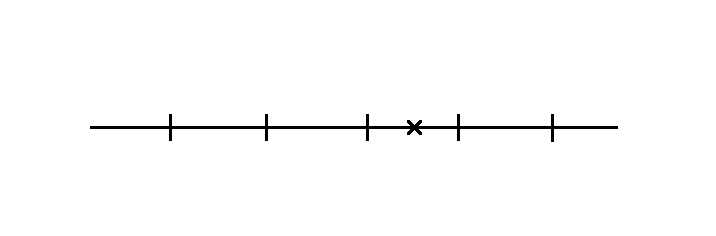
\includegraphics[width=\linewidth, height=1.5cm, right]{interpolation}
				\captionsetup{labelformat=empty}
				\put(-68, 27){$\gamma$}
				\put(-75, 16){$\underbrace{}$} 
				\put(-68, 0){$\delta$} \
				Идея заключается в интерполяции внутри интервалов $\delta$.
			\end{minipage}
		\end{center}
		тогда и только тогда, когда
		\[ \forall \varepsilon > 0 \quad \lim_{\delta \rightarrow 0} \limsup_{n \rightarrow \infty} \MP \bigg(\sup_{| \gamma_1 - \gamma_2 | < \delta} \| X_n(\gamma_1) - X_n(\gamma_2) \| \geq \varepsilon \bigg) = 0. \]
    \end{enumerate}
\end{rmrk}

\begin{thm}[\textbf{Асимптотическая эффективность оценок МП}] \label{Asymptotic efficiency ML estimators}
	Пусть $X_1, \dots, X_n$ i.i.d. $\sim P_\vartheta$, $\vartheta \in \Theta$, $\ell(\cdot, \vartheta)$ -- функция правдоподобия. Также:
	\begin{enumerate}
		\item $\Theta \subset \MR^k$ -- компактное пространство и $\vartheta \subset \mathrm{int}(\Theta)$.
		\item $\eta \mapsto \ell(x, \eta) $ непрерывна на $\Theta$ и дважды непрерывно дифференцируема по $\vartheta$ для почти всех $x \in \mathcal{X}$.
		\item Существуют функции $H_0, H_2 \in L^1(P_\vartheta)$ и $H_1 \in L^2(P_\vartheta)$, такие что:
		\[ \sup_{\eta \in \Theta} |\ell(x, \eta)| \leq H_0(x), \quad \sup_{\eta \in \Theta} \|\dot{\ell}(x, \eta)\| \leq H_1(x), \quad \sup_{\eta \in \Theta} \|\ddot{\ell}(x, \eta)\| \leq H_2(x) \quad \forall x \in \mathcal{X}. \]
		\item Информация Фишера
		\[ I(f(\cdot, \vartheta))=\ME_\vartheta[\dot{\ell}(X,\vartheta)\dot{\ell}(X,\vartheta)^T] \]
		положительно определенная (обратима).
	\end{enumerate}
	Тогда имеет место сходимость:
	\[ \sqrt{n}(\hat{\theta}_n-\vartheta) \convdistr \mathcal{N}(0, I(f(\cdot, \vartheta))^{-1}). \]
\end{thm}
\begin{proof} \\
	\textit{Шаг 1:} покажем состоятельность оценки $\hat{\theta}_n$ (проверим, что условия из Теоремы \ref{Consistency of ML estimator} соблюдаются)
	\begin{enumerate}
		\item Соблюдается по предположению.
		\item $\eta \mapsto L_n(\eta)$ п.н. непрерывная по условию (ii). Также, используя (ii), (iii) и мажорируемую сходимость, получаем
		\[ |L(\eta_1, \vartheta) - L(\eta_2, \vartheta)| \leq \int_{\mathcal{X}} |\ell(x, \eta_1) - \ell(x,\eta_2)| f(x,\vartheta) \mu(dx) \rightarrow 0,  \]
		при $\eta_1 \rightarrow \eta_2$.
		\item В силу Сильного Закона Больших Чисел:
		\[
		\begin{aligned}
		\limsup_{n \rightarrow \infty} \sup_{\| \eta_1 - \eta_2 \| < \delta} | L_n(\eta_1) - L_n(\eta_2)| & \leq \limsup_{n \rightarrow \infty} \frac{1}{n} \sum_{i=1}^{n} \sup_{\| \eta_1 - \eta_2 \| < \delta} |\ell(X_i, \eta_1) - \ell(X_i, \eta_2) |\\
		& = \ME_\vartheta[\sup_{\| \eta_1 - \eta_2 \| < \delta}|\ell(X,\eta_1) - \ell(X, \eta_2)|] \quad Q_\vartheta = \otimes_{i=1}^\MN P_\vartheta\text{-п.н.}
		\end{aligned}
		\]
		Так как $\Theta$ компакт, то $\eta \mapsto \ell(X, \eta)$ (п.н.) равномерно непрерывная. Как следствие, последнее выражение сходится к нулю при $\delta \rightarrow 0$ (используя снова мажорируемую сходимость).
	\end{enumerate}	

	\textit{Шаг 2:} пусть $A_n$ -- $k$-мерный прямоугольник с вершинами $\hat{\theta}_n$ и $\vartheta$. Поскольку $\hat{\theta}_n \xrightarrow{Q_\vartheta} \vartheta$ и $\vartheta \in \mathrm{int}(\Theta)$, то
	\[ Q_\vartheta(A_n \subset \mathrm{int}(\Theta)) \rightarrow 1. \]
	Также
	\[ \dot{L}_n(\hat{\theta}_n) = \frac{1}{n} \sum_{i=1}^{n} \dot{\ell}(X_i, \hat{\theta}_n) = 0 \]
	по определению $\hat{\theta}_n$.
	По Теореме о среднем:
	\[ -\dot{L}_n(\vartheta) = \dot{L}_n(\hat{\theta}_n) - \dot{L}_n(\vartheta) = \ddot{L}_n(\widetilde{\theta}_n)(\hat{\theta}_n - \vartheta) \]
	для некоторого $\widetilde{\theta}_n \in A_n$.
	Как и в Замечании \ref{rmrk2.25}:
	\[
	\begin{aligned}
	 \ME[\dot{\ell}(X_i, \vartheta)] & = \int_{\mathcal{X}} \dot{\ell}(x, \vartheta) f(x, \vartheta) \mu(dx) \\
	 \ell = \log f \rightarrow & = \int_{\mathcal{X}} \dot{f}(x, \vartheta) \mu(dx) = 0.
	\end{aligned}
	 \]
	 По определению
	 \[ \Cov(\dot{\ell}(X_i, \vartheta)) = I(f(\cdot, \vartheta)). \]
	 Тогда по Центральной Предельной Теореме:
	 \[ \sqrt{n} \dot{L}_n(\vartheta) \convdistr \mathcal{N}(0, I(f(\cdot, \vartheta))). \]
	 
	\textit{Шаг 3:} предположим, что
	\begin{equation} \label{eq5.3}
		\ddot{L}_n(\widetilde{\theta}_n) \xrightarrow{Q_\vartheta} -I(f(\cdot, \vartheta)).
	\end{equation}
	Если \eqref{eq5.3} соблюдается, мы можем заключить, что
	\[ \lim\limits_{n \rightarrow \infty} Q_\vartheta(\ddot{L}_n(\widetilde{\theta}_n) \text{ обратима}) = 1. \]
	Тогда, используя лемму Слуцкого, получаем
	\[
	\begin{aligned}
	\sqrt{n}(\hat{\theta}_n - \vartheta) & = -\ddot{L}_n(\widetilde{\theta}_n)^{-1} \dot{L}_n(\vartheta) 1_{ \{ A_n \subset \mathrm{int}(\Theta)
	 \} \cap \{ \ddot{L}_n(\widetilde{\theta}_n) \text{ обратима} \}} + B_n \\
	& \rightarrow I(f(\cdot, \vartheta))^{-1} \mathcal{N}(0, I(f(\cdot, \vartheta))) = \mathcal{N}(0, I(f(\cdot, \vartheta))^{-1}),
	\end{aligned}
	\]
	так как $B_n \xrightarrow{Q_\vartheta} 0$.
	
	\textit{Шаг 4:} докажем \eqref{eq5.3}. Используем равенство:
	\[ \ddot{\ell}(x, \vartheta) = \frac{\ddot{f}(x, \vartheta)}{f(x,\vartheta)} - \dot{\ell}(x, \vartheta)\dot{\ell}(x, \vartheta)^T. \]
	Тогда имеет место:
	\[\ME_\vartheta[\ddot{\ell}(X, \vartheta)] + I(f(\cdot, \vartheta)) = \ME_\vartheta\Big[ \frac{\ddot{f}(X, \vartheta)}{f(X,\vartheta)} \Big] = 0, \]
	как в Замечании \ref{rmrk2.25}. Из Закона Больших Чисел следует:
	\[ \ddot{L}_n(\vartheta) \xrightarrow{Q_\vartheta} - I(f(\cdot, \vartheta)). \]
	Наконец, используем равенство
	\[ \lim\limits_{\delta \rightarrow 0} \lim\limits_{n \rightarrow \infty} Q_\vartheta(\| \widetilde{\theta}_n - \vartheta \| < \delta) = 1 \]
	и непрерывность $\ddot{\ell}$ по $\vartheta$, чтобы завершить доказательство \eqref{eq5.3}.
\end{proof}

\begin{rmrk}
	Теорема \ref{Consistency of ML estimator} и Теорема \ref{Asymptotic efficiency ML estimators} -- это специальные случаи \textbf{\textit{оценок минимального контраста}}, которые минимизируют функцию
	\[ \eta \mapsto \frac{1}{n} \sum_{i=1}^{n}k(X_i, \eta). \]
	Можно получить похожие результаты при схожих предположениях, но асимптотическая эффективность достигается только при $k = -\ell$.
\end{rmrk}

\begin{exmp}
	Пусть $X_1, \dots, X_n$ i.i.d. $\sim Exp(\lambda)$. Найдем оценку максимального правдоподобия. Для этого
	\[f_n(X, \lambda) = \lambda^n \exp\bigg(-\lambda \sum_{i=1}^{n} X_i\bigg) 1_{[0, \infty)} (\min_{i=1}^n X_i) \]
	или
	\[\ell_n(X, \lambda) = n \log(\lambda) - \lambda \sum_{i=1}^{n} X_i + \log 1_{[0, \infty)} (\min_{i=1}^n X_i) \]
	должны быть максимизированы. Приравнивая любую из производных к нулю, получаем условие:
	\[\frac{n}{\lambda} = \sum_{i=1}^{n} X_i,  \]
	то есть оценка:
	\[\hat{\lambda}_n = \frac{1}{\overline{X}_n}. \]
	Рассчитаем информацию Фишера:
	\[ 
	\begin{aligned}
	\ell_1 (X, \lambda)&  = \log(\lambda) - \lambda X + \log(1_{[0, \infty)} X) \\
	&\Rightarrow \dot{\ell}_1(X, \lambda) = -\Big(X - \frac{1}{\lambda}\Big) \\
	&\Rightarrow I(f(\cdot, \lambda)) = \ME_\lambda\Big[\Big(X - \frac{1}{\lambda}\Big)^2\Big]. 
	\end{aligned}
	\]
	По Теореме \ref{Asymptotic efficiency ML estimators}
	\[ \sqrt{n}(\hat{\lambda}_n - \lambda) \convdistr \mathcal{N}(0, \lambda^2),  \]
	но с другой стороны:
	\[ \sqrt{n}\Big(\overline{X}_n - \frac{1}{\lambda}\Big) \convdistr \mathcal{N}\Big(0, \frac{1}{\lambda^2}\Big).  \]
	Используя Дельта-метод для $g(x) = x^{-1}$, получаем
	\[ \sqrt{n}(\overline{X}_n^{-1} - \lambda) \convdistr \mathcal{N}(0, \lambda^2). \]
	Также заметим, что
	\[ \Var_\lambda(\hat{\lambda}_n) = n^{-1} \lambda^2 = (n I(f(\cdot, \lambda)))^{-1} \]
	является следствием из Предположения \ref{prps2.31} для экспоненциального семейства.
\end{exmp}

\raggedbottom
\pagebreak
\section*{Упражнения}
\begin{exc}
	Докажите следующий вариант леммы Слуцкого: пусть $(X_n)$ и $(Y_n)$ -- последовательности вещественнозначных случайных величин, такие что
	\[X_n \convdistr X \quad \text{и} \quad Y_n \convprob c,  \]
	где $X$ -- вещественнозначная случайная величина и $c \in \MR$. Тогда имеет место:
	\[ X_n + Y_n \convdistr X + c. \]
	\textit{Подсказка}: последовательность $(Z_n)$ сходится к $Z$ тогда и только тогда, когда $\ME[f(Z_n)] \rightarrow \ME[f(Z)]$ для любых равномерно непрерывных и ограниченных функций $f:\MR \rightarrow \MR$.
\end{exc}

\begin{exc}
	Пусть $(X_n)$ -- последовательность i.i.d. случайных величин с плотностью
	\[ f(x, \vartheta) = \vartheta x^{\vartheta - 1} 1_{[0, 1]}(x). \]
	\begin{enumerate}
		\item Найдите оценку максимального правдоподобия $\hat{\vartheta}$.
		\item Рассчитайте асимптотическое распределение $\hat{\vartheta}$. \\
		\textit{Подсказка}: для $\vartheta > 0$:
		\[ \int_{0}^{1} \log(x) x^{\vartheta - 1} dx = -\frac{1}{\vartheta}, \quad \int_{0}^{1} (\log(x))^2x^{\vartheta - 1}dx = \frac{2}{\vartheta^3}.  \]
	\end{enumerate}
\end{exc}

\begin{exc}
	\textbf{\textit{Коэффициент вариации}} вероятностного распределения $P$ определяется как
	\[ c_v(X) := \frac{\sqrt{\Var(X)}}{\ME[X]},\ X \sim P, \]
	если соответствующие моменты существуют и $\ME[X] \neq 0$. Пусть $(X_n)$ -- последовательность i.i.d. нормально распределенных случайных величин: $X_i \sim \mathcal{N}(\mu, \sigma^2)$, где $\mu \in \MR / \{0\}$ и $\sigma^2 > 0$.
	\begin{enumerate}
		\item Найдите оценку $\hat{c}_n(X)$ для $c_v(X)$, полученную методом моментов.
		\item Выведите Центральную Предельную Теорему для оценки $\hat{c}_n(X)$.
	\end{enumerate}
\end{exc}

\begin{exc}
	Пусть $(X_n)$ -- последовательность i.i.d. равномерно распределенных случайных величин: $X_i \sim \mathcal{U}[0. \vartheta]$. Покажите, что $\big(\prod_{i=1}^{n} X_i \big)^{\frac{1}{n}}$ -- состоятельная оценка для $\frac{\vartheta}{e}$.\\
	\subitem \textit{Подсказка}: один из способов доказать сходимость по распределению, это показать, что
	\[ \sqrt{n} \bigg(\Big(\prod_{i=1}^{n} X_i \Big)^{\frac{1}{n}} - \frac{\vartheta}{e} \bigg) \convdistr \mathcal{N}\bigg(0, \Big(\frac{\vartheta}{e} \Big)^2\bigg). \]
\end{exc}

\begin{exc}
	Пусть $(X_n)$ -- последовательность i.i.d. $\mathcal{N}(\mu, 1)$ распределенных величин. Пусть также $a > 0$ и
	\[ \hat{\mu}_a =
	\left \{
	\begin{array}{cl}
	\overline{X}_n, & |\overline{X}_n| \geq n^{-\frac{1}{4}}, \\
	a\overline{X}_n, & \text{иначе}. 
	\end{array}
	\right.
	\]
	\begin{enumerate}
		\item Покажите, что
		\[ \sqrt{n}(\hat{\mu}_a - \mu) \convdistr \mathcal{N}(0, v(\mu)), \]
		где $v(\mu) = 1$, если $\mu \neq 0$, и $v(\mu) = a^2$, иначе.
		\item Для каких $a$ $\mu_a$ является эффективной?
		\item Покажите, что существуют случаи, для которых имеет место:
		\[ v(\mu) \leq I_1^{-1}(\mu). \]
	\end{enumerate}
\end{exc}
\graphicspath{{./chapters/chapter06/}}
\chapter{Основы тестирования}

В этой главе мы проверяем гипотезы о неизвестном параметре $\vartheta$. Как и ранее, мы рассматриваем статистический эксперимент $(\mathcal{X}, \mathcal{B}, \mathcal{P})$, где $\mathcal{P}=\{ P_\vartheta \mid \vartheta \in \Theta \}$.

\begin{exmp}
	Обсудим (упрощенный) клинический эксперимент, в которомы мы принимаем решение, лучше ли новоизобретенное лекарство B, чем известное лекарство А или нет. Предположим, что мы знаем по опыту предыдущих лет, что А имеет шанс излечения 65\%. Новое лекарство B было протестировано на 100 подопытных и 80\% выздоровели. Должны мы выбрать A или B? \\
	На языке математики мы проверяем:
	\[ H: p \leq 0.65 \quad \text{против} \quad K: p > 0.65, \]
	где $p$ -- неизвестная вероятность излечения после принятия лекарства B.
\end{exmp}

\begin{defn}
	Пусть $\Theta = \Theta_H \cup \Theta_K$  -- разделение параметрического пространства.
	\begin{enumerate}
		\item $\Theta_H$ называется \textbf{\textit{(нулевой) гипотезой}}, $\Theta_K$ называется \textbf{\textit{альтернативой}}.
		\item \textbf{\textit{Рандомизированный критерий}} -- измеримое отображение
		\[ \varphi:(\mathcal{X}, \mathcal{B}) \rightarrow ([0, 1], \mathcal{B}|_{[0,1]}). \]
		Функция $\varphi(x)$ -- это вероятность принятия решения, что $\vartheta \in \Theta_K$, после наблюдения $x=X(\omega)$. Множество таких критериев обозначим:
		\[ \Phi = \{ \varphi \mid \varphi \text{ -- рандомизированный критерий} \}. \]
		\item Для критерия $\varphi$ назовем $\mathcal{K}= \{x \mid \varphi(x)=1 \}$ \textbf{\textit{критической областью}}, а $\mathcal{R}= \{x \mid \varphi(x) \in (0,1) \}$ -- \textbf{\textit{областью рандомизации}}. Критерий $\varphi$ называется \textbf{\textit{нерандомизированным}}, если $\mathcal{R} = \emptyset$. 
	\end{enumerate}
\end{defn}

\begin{exmp} \label{exmp6.3}
	В ситуации в предыдущем примере мы знаем, что $\overline{X}_n$ является UMVU-оценкой $p$. Разумно принять $K$, если значение $\overline{X}_n$ достаточно большое, например:
	\[ \varphi(x) =
	\left \{
	\begin{array}{cl}
	1 & \overline{X}_n > 0.7 \\
	0 & \overline{X}_n \leq 0.7 
	\end{array}
	\right.
	\] 
	является разумным критерием.
\end{exmp}

\begin{rmrk}
	При принятии решения могут произойти две ошибки:
	\begin{itemize}
		\item Ошибка первого рода: отклонить гипотезу $H$, когда она верна.
		\item Ошибка второго рода: принять гипотезу $H$, когда она неверна.
	\end{itemize}
	\begin{center}
		\quad\quad\quad\quad\quad\quad\quad Истина \\
		Решение
		\begin{tabular}{| c | c | c|}
			\hline
			& $\Theta_H$ & $\Theta_K$ \\
			\hline
		 $\Theta_H$ & \checkmark & Ошибка 2-го рода \\
		\hline
			 $\Theta_K$ & Ошибка 1-го рода & \checkmark \\
			 \hline
		\end{tabular}
	\end{center}
	Обе ошибки могут произойти с определенными вероятностями.
\end{rmrk}

\begin{exmp}
	В Примере \ref{exmp6.3} вероятность принятия $K$:
	\[ P_p(\varphi(X)=1)=P_p(\overline{X}_n > 0.7). \]
	На практике биномиальное распределение можно аппроксимировать нормальным:
	\[
	\begin{aligned}
	P_p(\overline{X}_n > 0.7) & = P_p\bigg(\frac{\sqrt{n}(\overline{X}_n - p)}{\sqrt{p(1-p)}} > \frac{\sqrt{n}(0.7 - p)}{\sqrt{p(1-p)}}\bigg) \\
	\text{ЦПТ} \rightarrow & \approx P\bigg(\mathcal{N}(0,1) > \frac{\sqrt{n}(0.7 - p)}{\sqrt{p(1-p)}}\bigg) = \Phi\bigg(\frac{\sqrt{n}(0.7 - p)}{\sqrt{p(1-p)}}\bigg).
	\end{aligned}	 
	\]
	Используя Лемму Слуцкого, мы можем заменить $p$ на $\overline{X}_n$ в знаменателе. Пусть $n=100$ и $\overline{X}_n = 0.8$, тогда
	\[ P_p(\varphi(X)=1) \approx \Phi(25(p-0.7)).  \]
	Например, если $p \leq 0.65$:
	\[ P_p(\text{Ошибка первого рода}) \approx
	\left \{
	\begin{array}{cl}
	0, & p = 0.5 \\
	0.006, &  p = 0.6
	\end{array}
	\right.
	\]
	Вероятность ошибки ограничена сверху:
	\[ P_p(\text{Ошибка первого рода}) \leq P_{0.65}(\text{Ошибка первого рода}) \approx \Phi(1.25) \approx 0.106. \]
	Симметрично
	\[ P_p(\text{Ошибка второго рода}) \approx
	\left \{
	\begin{array}{cl}
	0, & p = 0.9 \\
	0.006, &  p = 0.8 \\
	0.5, & p = 0.7
	\end{array}
	\right.
	\]
	Граница сверху:
	\[ P_p(\text{Ошибка второго рода}) \leq P_{0.65}(\text{Ошибка второго рода}) \approx 0.894. \]
\end{exmp}

\begin{rmrk}
	В идеале, мы хотим минимизировать вероятности обеих ошибок и выбрать оптимальный критерий. Проблема заключается в том, что критерии
	\[ \varphi_0(X) \equiv 0 \Rightarrow
	\left \{
	\begin{array}{cl}
	P_p(\text{Ошибка первого рода}) = 0 \\
	P_p(\text{Ошибка второго рода}) = 1
	\end{array}
	\right.
	\]
	\[ \varphi_1(X) \equiv 1 \Rightarrow
	\left \{
	\begin{array}{cl}
	P_p(\text{Ошибка первого рода}) = 1 \\
	P_p(\text{Ошибка второго рода}) = 0
	\end{array}
	\right.
	\]
	являются оптимальными, если нужно минимизировать вероятность одной из ошибок, но они не минимизируют вероятности обеих ошибок одновременно. На практике берут границу $\alpha$ для вероятности ошибки первого рода и минимизируют вероятность ошибки второго рода по всем критериям. Обычно $0.01 \leq \alpha \leq 0.1$. 
\end{rmrk}

\begin{defn}
	Пусть $\varphi$ -- критерий для $H: \varphi \in \Theta_H \text{ против } K:\vartheta \in \Theta_K$.
	\begin{enumerate}
		\item Функция
		\[ \beta_\varphi:
		\left \{
		\begin{array}{ccl}
        \Theta & \rightarrow & [0, 1] \\
		\vartheta & \mapsto & \ME_\vartheta[\varphi(X)]
		\end{array}
		\right.
		\]
		называется \textbf{\textit{функцией мощности $\varphi$}}.
		\item Критерий $\varphi$ называется \textbf{\textit{критерием с уровнем значимости $\alpha$}} $\in [0, 1]$, если
		\[ \beta_\varphi(\vartheta) \leq \alpha \quad \forall \vartheta \in \Theta_H \]
		Зададим множество таких критериев:
		\[ \Phi_\alpha = \{ \varphi \in \Phi \ |\ \varphi \text{ -- критерий с уровнем значимости }\alpha  \}. \]
		\item Критерий $\varphi$ называется \textbf{\textit{несмещенным с уровнем значимости $\alpha$}} $\in [0, 1]$, если $\varphi \in \Phi_\alpha$ и
		\[ \beta_\varphi(\vartheta) \geq \alpha \quad  \forall \vartheta \in \Theta_K, \]
		\[  \Phi_{\alpha \alpha} = \{ \varphi  \in \Phi_\alpha \ |\ \varphi \text{ -- несмещенный критерий}  \}. \]
	\end{enumerate}
\end{defn}

\begin{rmrk} \
	\begin{enumerate}
		\item Если $\varphi$ -- нерандомизированный критерий, то
		\[ \beta_\varphi(\vartheta) = P_\vartheta(\varphi(X) = 1) \]
		-- вероятность принятия $K$. В частности,
		\begin{enumerate}
			\item $\vartheta \in \Theta_H$: $\beta_\varphi(\vartheta)$ -- вероятность ошибки 1-го рода.
			\item $\vartheta \in \Theta_K$: $1-\beta_\varphi(\vartheta)$ -- вероятность ошибки 2-го рода.
		\end{enumerate}
		Аналогичная интерпретация имеет место для радномизированных критериев.
		\item Критерий $\varphi$ ограничивает вероятность ошибки первого рода уровнем значимости $\alpha$ $\forall \vartheta \in \Theta_H$.
		\item Для несмещенного критерия $\varphi$ вероятность принятия гипотезы $K$ в случае, если $\vartheta \in \Theta_K$, не меньше, чем в случае, если $\vartheta \in \Theta_H$.
	\end{enumerate}
\end{rmrk}

\begin{exmp}
	Функция мощности критерия из Примера \ref{exmp6.3} будет приблизительно равна:
	\[ \beta_\varphi:
	\left \{
	\begin{array}{ccl}
	[0, 1] & \rightarrow & [0, 1] \\
	p & \mapsto & \beta_\varphi(p) \approx \Phi\Big(\frac{\sqrt{n}(p-0.7)}{\sqrt{\overline{X}_n (1-\overline{X}_n)}}\Big).
	\end{array}
	\right.
	\]
	Уровень значимости критерия $\varphi$: $\alpha \approx 0.106$.
\end{exmp}

\begin{defn} \
	\begin{enumerate}
		\item Критерий $\varphi^* \in \Phi_\alpha$ называется \textbf{\textit{равномерно наиболее мощным (UMP) с уровнем значимости $\alpha$}}, если
		\[\beta_{\varphi^*}(\vartheta) = \sup_{\varphi \in \Phi_\alpha} \beta_\varphi(\vartheta) \quad \forall \vartheta \in \Theta_K. \]
		\item Критерий $\varphi^* \in \Phi_{\alpha \alpha}$ называется \textbf{\textit{равномерно наиболее мощным несмещенным (UMPU) с уровнем значимости $\alpha$}}, если
		\[\beta_{\varphi^*}(\vartheta) = \sup_{\varphi \in \Phi_{\alpha\alpha}} \beta_\varphi(\vartheta) \quad \forall \vartheta \in \Theta_K. \]
	\end{enumerate}
\end{defn}

\begin{thm} \label{thm6.11}
	Пусть $\mathcal{P} = \{P_\vartheta\ |\ \vartheta \in \Theta  \}$ -- семейство распределений на $(\mathcal{X}, \mathcal{B})$, статистика $T:(\mathcal{X}, \mathcal{B}) \rightarrow (\mathcal{T}, \mathcal{D})$ -- достаточная для $\vartheta$ и $\varphi$ -- критерий. Тогда существует критерий $\psi \circ T$, обладающий той же функцией мощности, что и $\varphi$, а именно:
	\[ \psi \circ T = \ME[\varphi | T]. \]
\end{thm}
\begin{proof}
	Пусть $\psi(t) = \ME[\varphi | T = t]$. Во-первых, $\psi(T) \in [0, 1]$, так как это критерий. Также,
	\[ \beta_{\psi \circ T}(\vartheta) = \ME_\vartheta[\psi \circ T] = \ME_\vartheta[\ME[\varphi | T ]] = \ME_\vartheta[\varphi] = \beta_\varphi(\vartheta). \]
\end{proof}

\begin{rmrk} \
	\begin{enumerate}
		\item Теорема \ref{thm6.11} показывает, что для создания критерия всегда можно воспользоваться достаточной статистикой.
		\item Простейший случай простых гипотез:
		\[ H:\vartheta \in \{\vartheta_0 \}\quad \text{против} \quad K:\vartheta \in \{\vartheta_1 \}, \quad \vartheta_0 \neq \vartheta_1. \]
		Зададим доминирующую меру для $P_{\vartheta_0}$ и $P_{\vartheta_1}$:
		\[\mu = P_{\vartheta_0} + P_{\vartheta_1}. \]
		Также, пусть
		\[ p_i = \frac{dP_{\vartheta_i}}{d\mu} \]
		и 
		\[ \frac{p_1}{p_0} = 
		\left \{
		\begin{array}{cl}
		\infty, & p_1 > 0, p_0 = 0 \\
		\text{произвольное}, & p_1 = 0, p_0 = 0.
		\end{array}
		\right.
		\]
		Имеют место следующие утверждения:
		\begin{enumerate}
			\item Величина $\frac{p_1}{p_0}$ независима от $\mu$ (вплоть до множеств меры нуль).
			\item $\frac{p_1}{p_0}$ -- минимальная достаточная статистика для $\vartheta$ (Пример \ref{exmp4.20}).
			\item UMP-критерий с уровнем значимости $\alpha$ максимизирует
			\[ \beta_\varphi(\vartheta_1) = \ME_{\vartheta_1}[\varphi(X)] = \int \varphi(x) p_1(x) \mu(dx) \]
			при ограничении
			\[ \beta_\varphi(\vartheta_0) = \ME_{\vartheta_0}[\varphi(X)] = \int \varphi(x) p_0(x) \mu(dx) \leq \alpha. \]
		\end{enumerate}
	\end{enumerate}
\end{rmrk}

\begin{defn}
	В случае простой гипотезы критерий $\varphi$ называется \textbf{\textit{критерием Неймана-Пирсона (NP критерий)}}, если существует константа $c \in [0,\infty )$, такая что
	\[ \varphi(x):
	\left \{
	\begin{array}{cl}
	1, & p_1(x) > cp_0(x), \\
	0, & p_1(x) < cp_0(x).
	\end{array}
	\right.
	\]
\end{defn}

\begin{thm}[\textbf{\textit{NP лемма}}]
	Пусть $\Theta = \{ \vartheta_0, \vartheta_1 \}$ и рассматриваются гипотезы
	\[ H:\vartheta \in \{\vartheta_0 \}\quad \text{против} \quad K:\vartheta \in \{\vartheta_1 \}. \]
	\begin{enumerate}
		\item NP критерий $\varphi^*$ -- UMP-критерий с уровнем значимости $\alpha = \ME_{\vartheta_0}[\varphi^*(X)]$.
		\item Для любого $\alpha \in [0, 1]$ существует NP критерий $\varphi$, такой что $\ME_{\vartheta_0}[\varphi(X)] = \alpha$.
		\item Если $\varphi'$ -- UMP-критерий с уровнем значимости $\alpha$, то $\varphi'$ -- (п.н.) NP критерий. Если $\ME_{\vartheta_0}[\varphi'(X)] < \alpha$, то $\ME_{\vartheta_1}[\varphi'(X)]=1$.
	\end{enumerate}
\end{thm}
\begin{proof}
	\begin{enumerate}
		\item Пусть $\varphi^*$ -- NP критерий с константой $c^*$ и $\varphi$ -- другой критерий, такой что $\beta_\varphi(\vartheta_0) \leq \alpha = \beta_{\varphi^*}(\vartheta_0)$. Рассмотрим
		\[ \beta_{\varphi^*}(\vartheta_1) - \beta_\varphi(\vartheta_1) = \int (\varphi^* - \varphi) p_1 d\mu = \int (\varphi^* - \varphi)(p_1 - c^*p_0)d\mu + \int c^* p_0 (\varphi^* - \varphi) d\mu. \]
		Второй интеграл неотрицателен, так как его подинтегральное выражение: 
		\[c^*(\beta_{\varphi^*}(\vartheta_0) - \beta_\varphi(\vartheta_0)) \geq 0.\]
		 В первом интеграле:
		\[\varphi^* - \varphi > 0 \Longrightarrow \varphi^* > 0 \Longrightarrow p_1 \geq c^*p_0, \]
		\[\varphi^* - \varphi < 0 \Longrightarrow \varphi^* < 1 \Longrightarrow p_1 \leq c^*p_0 \]
		$\Longrightarrow (\varphi^* - \varphi)(p_1 - c^*p_0) \geq 0$ всегда.
		\item Для $c \in \MR$ зададим
			\begin{center}\centering
				\begin{minipage}{0.18\textwidth}
					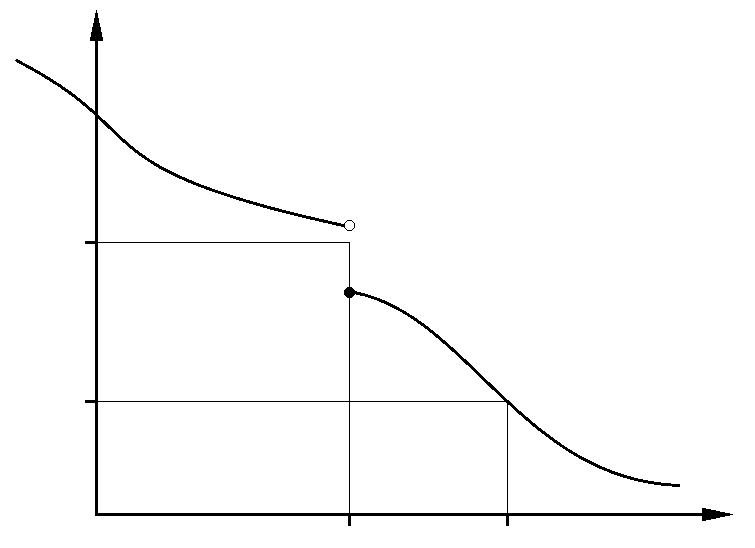
\includegraphics[width=\linewidth, right]{alpha}
					\captionsetup{labelformat=empty}
					\put (-90,32) {$\displaystyle \alpha_1 $}
					\put (-90,12) {$\displaystyle \alpha_2 $}
					\put (-49,-5) {$\displaystyle c_1 $}
					\put (0,-5) {$\displaystyle c $}
			        \put (-30,-5) {$\displaystyle c_2$}
					\put (-90,65) {$\displaystyle \alpha$}
				\end{minipage}
				\begin{minipage}{0.7\textwidth}
					\[ \alpha(c) := P_{\vartheta_0}\Big( \frac{p_1(X)}{p_0(X)} > c \Big). \]
					Очевидно, что $1 - \alpha(c)$ -- функция распределения. Для $\alpha \neq 0$ выберем $c^*$ таким образом, чтобы выполнялось соотношение
					\[ \alpha(c^*) \leq \alpha \leq \alpha(c^*-), \]
				\end{minipage}
			\end{center}
		где $\alpha(c-)$ обозначает левый предел в точке $c$. Для $\alpha = 0$ пусть $c^* = \infty$. Зададим функции
		\[ \gamma^*:
		\left \{
		\begin{array}{cl}
		\frac{\alpha - \alpha(c^*)}{\alpha(c^*-)-\alpha(c^*)}, & \text{если $\alpha(c^*-)-\alpha(c^*) > 0$}, \\
		0, & \text{иначе}.
		\end{array}
		\right.
		\]
		и
		\[ \varphi^*(x):
		\left \{
		\begin{array}{cl}
		1, & p_1(x) > c^* p_0(x), \\
		\gamma^*, & p_1(x) = c^*p_0(x), \\
		0, & p_1(x) < c^* p_0(x).
		\end{array}
		\right.
		\]
		Если $c^* < \infty$, то
		\[ \beta_{\varphi^*}(\vartheta_0) = \int_{\{p_1 > c^* p_0\}}dP_{\vartheta_0} + \int_{\{p_1 = c^* p_0\}}\gamma^* dP_{\vartheta_0} = \alpha(c^*)+\gamma^*(\alpha(c^*-)-\alpha(c^*)) = \alpha. \]
		Если $c^* = \infty$, то
		\[\beta_{\varphi^*}(\vartheta_0) = P_{\vartheta_0}(p_1(X) > \infty) = 0. \]
		\item Пусть $\varphi'$ -- UMP-критерий с уровнем значимости $\alpha$ и $\varphi^*$ -- критерий из (ii). Так как из (i) следует, что $\varphi^*$ -- UMP, то $\beta_{\varphi^*}(\vartheta_1) = \beta_{\varphi_1}(\vartheta_1)$. Таким образом,
		\[ \int (\varphi^* - \varphi')p_1 d\mu = 0, \]
		но
		\[
		\int (\varphi^* - \varphi')p_1 d\mu = \int (\varphi^* - \varphi')(p_1 - c^*p_0)d\mu + \int c^*p_0(\varphi^* - \varphi')d\mu = I+II \]
		Так как $\beta_{\varphi^*}(\vartheta_0)=\alpha \geq \beta_{\varphi'}(\vartheta_0)$, второй интеграл неотрицателен. Как и в доказательстве (i), мы можем показать, что $I \geq 0$. Следовательно, $I = II = 0$. Зададим множество
		\[ S= \{ x\ |\ \varphi'(x) \neq \varphi^*(x) \} \cap \{ x\ |\ p_1(x) \neq c^*p_0(x) \}. \]
		На множестве $S$ имеет место неравенство
		\[ (\varphi^* - \varphi')(p_1 - c^*p_0)>0 \]
		$\Longrightarrow \mu(S) = 0$. На его дополнении $S^c$ $\varphi'$ -- NP критерий. Так как $II = 0$, либо $c^* = 0$, либо $\beta_{\varphi'}(\vartheta_0) = \beta_{\varphi^*}(\vartheta_0) = \alpha$. Если $\beta_{\varphi'}(\vartheta_0) < \alpha$, то $c^* = 0$ и $\varphi^*(x) = 1$ для любого $x$, такого что $p_1(x) > 0$. Следовательно,
		\[\beta_{\varphi^*}(\vartheta_1) = \int \varphi^*p_1 d\mu = \int p_1 d\mu = 1. \]
		Утверждение следует из равенства $\beta_{\varphi'}(\vartheta_1) = \beta_{\varphi^*}(\vartheta_1) = 1$.
	\end{enumerate}
\end{proof}

\begin{rmrk}
	NP критерий $\varphi^*$ для $H:\vartheta = \vartheta_0$ против $K:\vartheta = \vartheta_1$ на дополнении множества $S_= =\{x\ |\ p_1(x) = c^*p_0(x) \}$ определен единственным образом. На множестве $S_=$ критерий может быть выбран таким образом, чтобы $\beta_{\varphi^*}(\vartheta_0) = \alpha$. Один из возможных способов показан в пункте (ii). 
\end{rmrk}

\begin{crlr} \label{crlr6.16}
	Любой NP критерий $\varphi^*$, такой что $\beta_{\varphi^*}(\vartheta_0) \in (0, 1)$ является несмещенным. В частности,
	\[ \alpha:=\beta_{\varphi^*}(\vartheta_0) < \beta_{\varphi^*}(\vartheta_1). \]
\end{crlr}
\begin{proof}
	Критерий вида $\varphi \equiv \alpha$ имеет уровень значимости $\alpha$. Так как $\varphi^*$ -- UMP, $\beta_\varphi(\vartheta_1) \leq \beta_{\varphi^*}(\vartheta_1)$. Также заметим, что если $\alpha = \beta_{\varphi^*}(\vartheta_1) < 1$, то $\varphi$ -- UMP. Так как любой UMP-критерий является NP критерием, то имеет место равенство $p_1(x) = c^*p_0(x)$ для почти всех $x$. Следовательно, $c^*=1$ и $p_1 =p_0$ $\mu$-п.н., и также $P_{\vartheta_0} = P_{\vartheta_1}$ -- мы приходим к противоречию.
\end{proof}

\begin{exmp} \label{exmp6.17}
	Пусть $X_1, \dots, X_n$ i.i.d. $\sim \mathcal{N}(\mu, \sigma^2)$ с известным параметром $\sigma^2$. Рассмотрим гипотезы:
	\[ H:\mu = \mu_0 \quad \text{против} \quad K: \mu = \mu_1, \]
	где $\mu_0 < \mu_1$. Плотность $X_1, \dots, X_n$:
	\[ p_j(x) = (2 \pi \sigma^2)^{-n/2} \exp \Big \{ -\frac{1}{2\sigma^2} \Big( \sum_{i=1}^{n} X_i^2 - 2 \mu_j \sum_{i=1}^{n}X_i + n\mu_j^2  \Big)\Big \}, \quad j = 0, 1.  \]
	Неравенство для отношения плотностей (или отношения правдоподобия), необходимое для создания NP критерия:
	\[ \frac{p_1(x)}{p_0(x)} = \exp \Big \{ \frac{1}{\sigma^2} \sum_{i=1}^{n} x_i(\mu_1 - \mu_0) \Big \} \cdot f(\sigma^2, \mu_1, \mu_0) > c^*,  \]
	где $f(\sigma^2, \mu_1, \mu_0)$ -- известная положительная константа. Это неравенство эквивалентно:
	\[ \overline{X}_n = \frac{1}{n} \sum_{i=1}^{n}X_i > c, \]
	где $c$ -- соответствующая константа. Таким образом, достаточно найти $c$, такую что
	\[P_{\mu_0}(\overline{X}_n > c) = \alpha\]
	или, что эквивалентно,
	\[
	\begin{aligned}
	P_{\mu_0}\Big( &\underbrace{\frac{\sqrt{n}(\overline{X}_n - \mu_0)}{\sigma}} > \frac{\sqrt{n}(c-\mu_0)}{\sigma}\Big) = 1 - \Phi\Big(\frac{\sqrt{n}(c - \mu_0)}{\sigma}\Big) = \alpha. \\
	&\quad \sim \mathcal{N}(0, 1)
	\end{aligned}
	\]
	Назовем величину $u_\beta$ \textbf{\textit{$\beta$-квантилем}} стандартного нормального распределения $\mathcal{N}(0,1)$, если $\Phi(u_\beta) = \beta$. Тогда
	\begin{center}\centering
		\begin{minipage}{0.7\textwidth}
		  \[\frac{\sqrt{n}(c - \mu_0)}{\sigma} = u_{1-\alpha} \quad \Longleftrightarrow \quad c = \mu_0 + u_{1-\alpha}\frac{\sigma}{\sqrt{n}},  \]
		  и NP критерий:
		\end{minipage}
		\begin{minipage}{0.18\textwidth}
			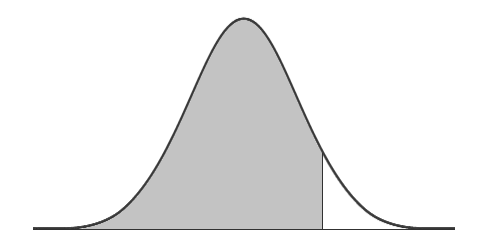
\includegraphics[width=\linewidth, right]{quantile}
			\captionsetup{labelformat=empty}
			\put (-28,32) {$\displaystyle \Phi(u_\beta) = \beta $}
			\put (-38,22) {\large $\swarrow$}
			\put (-33,-5) {$\displaystyle u_\beta $}
		\end{minipage}
	\end{center}
	\[\varphi^*(x) = 1_{\{\overline{X}_n > \mu_0 + u_{1-\alpha} \frac{\sigma}{\sqrt{n}}  \} }. \]
\end{exmp}

\begin{exmp} \label{exmp6.18}
	 Пусть $X_1, \dots X_n$ i.i.d. $\sim \mathcal{U}[0, \vartheta]$ и мы проверяем
	 \[ H:\vartheta=\vartheta_0 \quad \text{против} \quad K:\vartheta = \vartheta_1, \]
	 где $\vartheta_0 < \vartheta_1$. Плотности:
	 \[p_j(x) = \Big(\frac{1}{\vartheta_j}\Big)^n 1_{[0, \vartheta_j]} (x_{(n)}), \quad j=0,1, \]
	 и их отношение правдоподобия:
	 \[ \frac{p_1(x)}{p_0(x)}=
	 \left \{
	 \begin{array}{cl}
	 \Big(\frac{\vartheta_0}{\vartheta_1}\Big)^n, & x_{(n)} \leq \vartheta_0, \\
	 \infty, & x_{(n)} \in (\vartheta_0, \vartheta_1], \\
	 \text{произвольное}, & \text{иначе}.
	 \end{array}
	 \right.
	 \]
	 Далее
	 \[\alpha(c)  = P_{\vartheta_0}(p_1(X) > cp_0(X)) = 
	 \left \{
	 \begin{array}{cl}
	 1, & c \leq \Big(\frac{\vartheta_0}{\vartheta_1}\Big)^n, \\
	 0, & c > \Big(\frac{\vartheta_0}{\vartheta_1}\Big)^n.
	 \end{array}
	 \right.
	 \]
	 Для любого $\alpha \in (0, 1)$ имеет место
	 \[ \alpha(c) \leq \alpha \leq \alpha(c-) \quad \Longleftrightarrow \quad c = c^* = \Big(\frac{\vartheta_0}{\vartheta_1}\Big)^n.  \]
	 NP лемма гласит, что
	 \[ \varphi^*(x)=1_{\big\{\frac{p_1(x)}{p_0(x)} > c^*\big \}} + \gamma(x)1_{\big\{\frac{p_1(x)}{p_0(x)} = c^*\big \}} = 1_{\{x_{(n)}>\vartheta_0\}} + \gamma(x)1_{\{x_{(n)} \leq \vartheta_0\}}. \]
	 Как выбрать $\gamma(x)$? Возможностей много:
	 \[
	 \begin{aligned}
	 \varphi_1(x) = & 1_{\{x_{(n)} > c_1\}}, \quad c_1 = \vartheta_0 \sqrt[n]{1-\alpha}, \\
	 \varphi_2(x) = & 1_{\{x_{(n)} > \vartheta_0\}} + 1_{\{x_{(n)} < c_2\}}, \quad c_2 = \vartheta_0 \sqrt[n]{\alpha}, \\
	 \varphi_3(x) = & 1_{\{x_{(n)} > \vartheta_0\}} + \alpha1_{\{x_{(n)} \leq \vartheta_0\}}.
	 \end{aligned}
	 \]
\end{exmp}

\begin{rmrk}
	Простые гипотезы на практике не актуальны, но
	\begin{enumerate}
		\item Они дают интуитивное ощущение того, как нужно строить критерии. Во-первых, нужен т.н. \textbf{\textit{доверительный интервал}} $c(X) \subset \Theta$, внутри которого неизвестный параметр лежит с вероятностью $1-\alpha$. В Примере \ref{exmp6.17} мы использовали, что для $c(X)=[\overline{X}_n -u_{1 - \alpha} \frac{\sigma}{\sqrt{n}}, \infty)$ имеет место
		\[P_{\mu_0}(\mu_0 \in c(X)) = P_{\mu_0}(\overline{X}_n \leq \mu_0 + \frac{\sigma}{\sqrt{n}} u_{1-\alpha}) = 1-\alpha. \]
		Любой такой интервал  $c(X)$ может быть использован для построения критерия, например:
		\[c'(X) =\Big[\overline{X}_n -u_{1-\frac{\alpha}{2}} \frac{\sigma}{\sqrt{n}}, \overline{X}_n + u_{1-\frac{\alpha}{2}} \frac{\sigma}{\sqrt{n}} \Big].\]
		В дополнение, простые гипотезы показывают в какой стороне лежит альтернатива, и поэтому был выбран интервал $c(X)$ в Примере \ref{exmp6.17}.
		\item С помощью формальных результатов, таких как NP лемма, можно вывести более актуальные результаты.
	\end{enumerate}
\end{rmrk}

\begin{defn}
	Пусть $\Theta \subset \MR$, $\mathcal{P} = \{P_\vartheta\ |\ \vartheta \in \Theta \}$ и $T:(\mathcal{X},\mathcal{B}) \rightarrow (\MR,\mathcal{B})$ -- статистика. Семейство $\mathcal{P}$ называется \textbf{\textit{классом с монотонным (изотоническим) отношением правдоподобия}}, если для любого $\vartheta < \vartheta_1$ существует монотонно возрастающая функция $H_{\vartheta_0, \vartheta_1}: \MR \rightarrow [0, \infty)$, такая что
	\[\frac{p_{\vartheta_1}(x)}{p_{\vartheta_0}(x)} =H_{\vartheta_0, \vartheta_1}(T(x)) \quad P_{\vartheta_0} + P_{\vartheta_1}\text{-п.н.} \]
\end{defn}

\begin{exmp} \
	\begin{enumerate}
		\item В Примере \ref{exmp6.17}
		\[ \frac{p_{\mu_1}(x)}{p_{\mu_0}(x)} = \exp \Big \{ \frac{1}{\sigma^2} \sum_{i=1}^{n} x_i(\mu_1 - \mu_0) \Big \} \cdot f(\sigma^2, \mu_1, \mu_0),  \]
		монотонно возрастает по $\overline{x}_n$. Это свойство может быть обобщено до однопараметрических экспоненциальных семейств.
		\item В Примере \ref{exmp6.18}
		\[ \frac{p_{\vartheta_1}(x)}{p_{\vartheta_0}(x)} = \Big( \frac{\vartheta_0}{\vartheta_1} \Big)^n 1_{[0, \vartheta_0]}(x_{(n)}) + \infty 1_{(\vartheta_0, \vartheta_1]}(x_{(n)}) \]
		монотонно возрастает по $x_{(n)}$.
	\end{enumerate}
\end{exmp}

\begin{thm} \label{thm6.22}
	Пусть $\mathcal{P} = \{ P_\vartheta\ |\ \vartheta \in \Theta \}$ -- класс с монотонным отношением правдоподобия по $T$, $\vartheta_0 \in \Theta$ и  $\alpha \in (0, 1)$. Также, пусть
		\begin{center}\centering
			\begin{minipage}{0.7\textwidth}
				\[ \varphi^*(x) = 1_{\{T(x) > c\}} + \gamma 1_{\{ T(x) = c\}}, \]
				где
				\[ c := \inf \{t\ |\ P_{\vartheta_0}(T(X) > t) \leq \alpha \} \]
				и
				\[\gamma = 
				\left \{
				\begin{array}{cl}
				\frac{\alpha - P_{\vartheta_0}(T(X) > c) }{ P_{\vartheta_0}(T(X) = c) }, & \text{если } P_{\vartheta_0}(T(X) = c) \neq 0  \\
				0, & \text{иначе}.
				\end{array}
				\right.
				\]
			\end{minipage}
			\begin{minipage}{0.18\textwidth}
				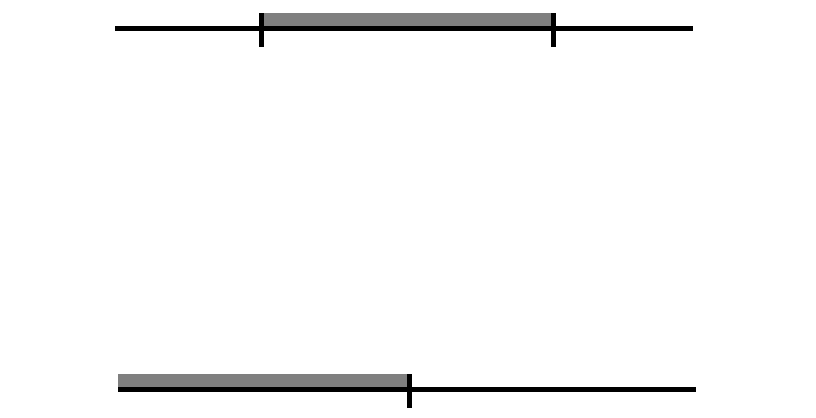
\includegraphics[width=\linewidth, right]{hypotheses}
				\captionsetup{labelformat=empty}
				\put (-105,10) {односторонние гипотезы:}
				\put (-30,-8) {$\displaystyle K$}
				\put (-65,-8) {$\displaystyle H$}
				\put (-103,50) {двусторонние гипотезы:}
				\put (-48,30) {$\displaystyle H$}
				\put (-75,30) {$\displaystyle K$}
				\put (-25,30) {$\displaystyle K$}
			\end{minipage}
		\end{center}
	Тогда 
	\begin{enumerate}
		\item $\beta_{\varphi^*}(\vartheta_0) = \alpha$ и $\varphi^*$ -- UMP-критерий с уровнем значимости $\alpha$ для односторонних гипотез:
		\[ H:\vartheta \leq \vartheta_0 \quad \text{против} \quad K:\vartheta > \vartheta_0. \]
		\item Для любого $\vartheta < \vartheta_0$ имеет место равенство
		\[ \beta_{\varphi^*}(\vartheta) = \inf \{ \beta_\varphi(\vartheta)\ |\ \varphi \in \Phi \text{ и } \beta_\varphi(\vartheta_0) = \alpha \}. \]
		\item Функция мощности $\vartheta \mapsto \beta_{\varphi^*}(\vartheta)$ строго монотонно возрастает для любого $\vartheta$, такого что $\beta_{\varphi^*}(\vartheta) \in (0,1)$.
		\item Для любого $\vartheta' \in \Theta$ $\varphi^*$ -- UMP-критерий с уровнем значимости $\alpha' = \ME_{\vartheta'}[\varphi^*(X)]$ для гипотез
		\[H': \vartheta \leq \vartheta' \quad \text{против} \quad K': \vartheta > \vartheta'. \]
    \end{enumerate}
\end{thm}
\begin{proof} \
	\begin{enumerate}
		\item Если $P_{\vartheta_0}(T(X) = c) = 0$, то
		\[\beta_{\varphi^*}(\vartheta_0) = P_{\vartheta_0}(T(X) > c) = \alpha.  \]
		Если $P_{\vartheta_0}(T(X) = c) > 0$, то мы подбираем $\gamma$ таким образом, чтобы имело место равенство
		\[\beta_{\varphi^*}(\vartheta_0)=P_{\vartheta_0}(T(X)>c) + \gamma P_{\vartheta_0}(T(X) = c) = \alpha. \]
		Пусть $\vartheta_0 < \vartheta_1$ и $H_{\vartheta_0, \vartheta_1}(T(x)) = p_{\vartheta_1}(x) / p_{\vartheta_0}(x)$. Вследствие монотонности
		\[ H_{\vartheta_0, \vartheta_1}(T(x)) \lessgtr H_{\vartheta_0, \vartheta_1}(c) = s \quad \Longrightarrow \quad T(x) \lessgtr c \]
		и
		\[ \varphi^*(x) =
		\left \{
		\begin{array}{cl}
		1, & H_{\vartheta_0, \vartheta_1}(x) > s, \\
		0, & H_{\vartheta_0, \vartheta_1}(x) < s.
		\end{array}
		\right.
	    \]
	    Таким образом $\varphi^*$ -- NP критерий с уровнем значимости $\alpha$ и по NP лемме
	    \[ \beta_{\varphi^*}(\vartheta') = \sup \{\beta_\varphi(\vartheta_1)\ |\ \varphi \in \Phi \text{ и } \beta_\varphi(\vartheta_0) = 1-\alpha \}. \]
	    Так как $\varphi^*$ не зависит от выбора $\vartheta_1$, это соотношение имеет место для любого $\vartheta_1 > \vartheta_0$. Наконец, пусть $\varphi'(x) = 1 - \varphi^*(x)$. Используя те же рассуждения, что и выше, можно показать, что
	    \[ \beta_{\varphi'}(\vartheta_2) = \sup \{\beta_\varphi(\vartheta_2)\ |\ \varphi \in \Phi \text{ и } \beta_\varphi(\vartheta_0) = \alpha \} \quad \forall \vartheta_2 < \vartheta_0. \]
	    Так как критерий вида $\overline{\varphi} \equiv \alpha$ удовлетворяет равенству $\beta_{\overline{\varphi}}(\vartheta_0) = \alpha$, мы заключаем, что
	    \[1 - \beta_{\varphi^*}(\vartheta_2) = \beta_{\varphi'}(\vartheta_2) \geq \beta_{1-\overline{\varphi}}(\vartheta_2) = 1 -\beta_{\overline{\varphi}}(\vartheta_2) = 1 - \alpha.   \]
	    Следовательно, $\beta_{\varphi^*}(\vartheta_2) \leq \alpha$ и $\varphi^* \in \Phi_\alpha$.
		\item Утверждение следует непосредственно, так как $\beta_{\varphi'} = 1 - \beta_{\varphi^*}$.
		\item Следует из Следствия \ref{crlr6.16}, так как для любых $\vartheta_1 < \vartheta_2$ $\varphi^*$ -- NP критерий.
		\item Доказывается, используя схожие аргументы, что и в доказательстве пункта (i).
	\end{enumerate}
\end{proof}

\begin{exmp}
	Пусть $X_1, \dots X_n$ i.i.d. $\sim \mathcal{N}(\mu, \sigma^2)$ с известным параметром $\sigma^2$. Из Примера \ref{exmp6.17} мы знаем, что плотности
	\[p_\mu(x) = (2 \pi \sigma^2)^{-\frac{n}{2}} \exp \Big\{ -\frac{1}{2\sigma^2}\sum_{i=1}^{n}(x_i - \mu)^2 \Big\} \]
	обладают монотонным отношением правдоподобия по $T(x) = \overline{x}_n$. Из Теоремы \ref{thm6.22}: UMP-критерий с уровнем значимости $\alpha$ для
	\[ H:\mu \leq \mu_0 \quad \text{против} \quad K:\mu > \mu_0  \]
	имеет вид
	\[ \varphi^*(x) = 1_{\{\overline{x}_n > c\}} + \gamma 1_{\{\overline{x}_n = c\}}. \]
	Так как $P_{\mu_0}(T(X) = c) = 0$, то $\gamma = 0$ и выбрать $c$ так, что $P_{\mu_0}(\overline{X}_n > c) = \alpha \Longleftrightarrow c = \mu_0 + \frac{\sigma}{\sqrt{n}} u_{1-\alpha}$. UMP-критерий
	\[ \varphi^*(x) = 1_{\{\overline{X}_n > \mu_0 + \frac{\sigma}{\sqrt{n}}u_{1-\alpha} \} } \]
	называется \textbf{\textit{односторонним критерием Гаусса}}.
\end{exmp}

\begin{rmrk} \
	\begin{enumerate}
		\item Существует эвристика, как получить односторонний критерий Гаусса: так как $\overline{X}_n$ UMVU-оценка для $\mu$, разумной стратегией будет принятие гипотезы $K$, если $\overline{X}_n$ достаточно большое. Следовательно, критерий должен иметь вид:
		\[\varphi(x) = 1_{\{\overline{X}_n > c\}}.  \]
		Выбираем $c$, контролируя вероятность ошибки первого рода. Для любого $\mu \leq \mu_0$ имеет место
		\[ \beta_\varphi(\mu) = P_\mu(\overline{X}_n > c) = P_\mu \Big( \frac{\sqrt{n}(\overline{X}_n - \mu) }{\sigma} > \frac{\sqrt{n}(c-\mu)}{\sigma}\Big) = 1 - \Phi\Big(\frac{\sqrt{n}(c-\mu)}{\sigma}\Big) \leq 1 - \Phi\Big(\frac{\sqrt{n}(c-\mu_0)}{\sigma}\Big).\]
		Мы должны удостовериться, что:
		\[ 1- \Phi\Big(\frac{\sqrt{n}(c-\mu_0)}{\sigma}\Big) \leq \alpha, \]
		иначе говоря:
		\[c \geq \mu_0 + \frac{\sigma}{\sqrt{n}} u_{1-\alpha}.\] 
		Мы берем $c = \mu_0 + \frac{\sigma}{\sqrt{n}} u_{1-\alpha}$, чтобы вероятность ошибки первого рода была равна $\alpha$.
		\item Этот метод позволяет построить критерий, однако ничего не говорит о его оптимальности. Что важно, он может быть применен в более общих ситуациях, например в случае неизвестного параметра $\sigma^2$. В такой ситуации можно воспользоваться оценкой
		\[ \hat{\sigma}_n^2 = \frac{1}{n-1}\sum_{i=1}^{n}(X_i - \overline{X}_n)^2. \]
		Как и выше, мы получаем:
		\[ \beta_\varphi(\mu) = P_\mu\Big( \frac{\sqrt{n}(\overline{X}_n - \mu) }{\hat{\sigma}_n} > \frac{\sqrt{n}(c-\mu)}{\hat{\sigma}_n}\Big) = 1 - F_{t_{n-1}}\Big( \frac{c - \mu}{\sqrt{\hat{\sigma}_n^2 / n}} \Big)  \]
		из Следствия \ref{crlr2.21}, где $F_{t_{n-1}}$ -- функция распределения $t_{n-1}$. Разумный выбор константы:
		\[ c = \mu_0 + \frac{\hat{\sigma}_n}{\sqrt{n}}t_{n-1,1-\alpha}, \]
		где $t_{n-1, 1-\alpha}$ -- $1-\alpha$-квантиль распределения Стьюдента с $n-1$ степенями свободы. Критерий
		\[ 1_{\{ \overline{x}_n > \mu_0 + \frac{\hat{\sigma}_n}{\sqrt{n}}t_{n-1,1-\alpha} \}} \]
		называется \textbf{\textit{односторонним t-критерием}}.
	\end{enumerate}
\end{rmrk}

\begin{rmrk}
	В общем случае не существует UMP-критериев для
	\[ H:\vartheta = \vartheta_0 \quad \text{против} \quad K:\vartheta \neq \vartheta_0, \]
	так как этот критерий должен быть оптимальным для всех
	\[ H':\vartheta = \vartheta_0 \quad \text{против} \quad K':\vartheta = \vartheta_1, \]
	где $\vartheta_0 \neq \vartheta_1$.
	В случае монотонного отношения правдоподобия оптимальный критерий будет
	\[ \varphi(x) = 1_{\{ T(x) > c \}} + \gamma(x) 1_{\{T(x) = c\}} \]
	для $\vartheta_1 > \vartheta_0$ и
	\[ \varphi'(x) = 1_{\{ T(x) < c'\}} + \gamma'(x) 1_{\{T(x) = c'\}} \]
	для $\vartheta_1 < \vartheta_0$, что невозможно.
\end{rmrk}

\begin{thm} \label{thm6.26}
	Пусть $\mathcal{P} = \{ P_\vartheta\ |\ \vartheta \in \Theta \}$ -- однопараметрическое экспоненциальное семейство с $\mu$-плотностью
	\[p_\vartheta(x) = c(\vartheta)h(x)\exp(Q(\vartheta) T(x)) \]
	с возрастающей функцией $Q$. Тогда существует UMPU-критерий для
	\[ H:\vartheta \in [\vartheta_1, \vartheta_2] \quad \text{против} \quad K:\vartheta \notin [\vartheta_1, \vartheta_2], \]
	а именно
	\[ \varphi^*(x) = 
	\left \{
	\begin{array}{cl}
	1, & \text{если } T(x) \notin [c_1, c_2], \\
	\gamma_i, & \text{если } T(x) = c_i, \\
	0, & \text{если } T(x) \in (c_1, c_2),
	\end{array}
	\right.
	\]
	где константы $c_i$, $\gamma_i$ определяются из равенства
	\[ \beta_\varphi(\vartheta_1) = \beta_\varphi(\vartheta_2) = \alpha \]
\end{thm}
\begin{proof}
	Теорема 3.7.1 в \cite{LehmannRomano}.
\end{proof}

\begin{rmrk}
	Похожие утверждения имеют место для $k$-параметрических экспоненциальных семейств.
\end{rmrk}

\raggedbottom
\pagebreak

\section*{Упражнения}
\begin{exc}
	Пусть $X_1, \dots, X_n$ -- i.i.d. нормально распределенные случайные величины: $X_i \sim \mathcal{N}(\mu, \sigma^2)$ с известным математическим ожиданием $\mu \in \MR$ и неизвестной дисперсией $\sigma^2 > 0$. Постройте UMP-критерий с уровнем значимости $\alpha \in (0, 1)$ для гипотез
	\[H: \sigma^2 < \sigma_0^2 \quad \text{против} \quad K:\sigma \geq \sigma_0^2.  \]
\end{exc}

\begin{exc}
	Пусть мы наблюдаем $X \in (0, 1)$. Постройте UMP-критерий с уровнем значимости $\alpha$ для
	\[H:\text{плотность $X$: } f(x) = 4x1_{(0, 1/2)}(x) + (4 - 4x)1_{(1/2, 1)}(x) \]
	против альтернативы
	\[ K: X \sim \mathcal{U}(0, 1).\]
\end{exc}

\begin{exc}
	Пусть $X$ -- случайная величина с плотностью
	\[ f_\vartheta(x) = \frac{2(\vartheta - x)}{\vartheta^2}1_{(0, \vartheta)}(x). \]
	Постройте UMP-критерий с уровнем значимости $\alpha$ для гипотез
	\[H: \vartheta = \vartheta_0 \quad \text{против} \quad K:\vartheta = \vartheta_1 \]
	для $\vartheta_1 < \vartheta_0$.
\end{exc}

\begin{exc} \label{exc6.4}
	Пусть $X_1, \dots, X_n$ -- i.i.d. экспоненциально распределенные случайные величины: $X_i \sim Exp(\vartheta)$, т.е. плотность $X_i$:
	\[ f_\vartheta(x) = \vartheta \exp (\vartheta x) 1_{[0, \infty)}(x).  \]
	\begin{enumerate}
		\item Покажите, что распределение $X = (X_1, \dots, X_n)$ обладает мононотонным отношением правдоподобия.
		\item Постройте UMP-критерий для гипотез
		\[H: \vartheta < \vartheta_0 \quad \text{против} \quad K:\vartheta \geq \vartheta_0.  \]
		\item Рассчитайте критическую область для этого критерия для $\vartheta_0 = 1$, $n = 10$ и $\alpha = 0.05$.
		\subitem \textit{Подсказка}: 5\%-квантиль гамма распределения $\Gamma(10, 1)$ приблизительно равен 5.43.
		\end{enumerate}
\end{exc}

\begin{exc}
	Рассмотрим еще раз ситуацию из Упражнения \ref{exc6.4}.
	\begin{enumerate}
		\item Рассмотрим гипотезы
		\[ H:\vartheta = \vartheta_0 \quad \text{против} \quad K:\vartheta \neq \vartheta_0. \]
		Обрисуйте построение доверительного интервала $[\overline{X}_n - \alpha, \overline{X}_n + \alpha]$ с уровнем значимости $\alpha$ для $\gamma(\vartheta) = 1/ \vartheta$. Как он поможет для построения критерия для гипотез выше?
		\item Используйте аппроксимацию нормальным распределением, чтобы построить доверительный интервал из (i) для $n=100$ и $\alpha = 0.1$.
	\end{enumerate}
\end{exc}

\begin{exc}
	Продолжим рассмотрение Упражнения \ref{exc6.4}.
	\begin{enumerate}
		\item Пусть $n=1$. Постройте UMPU-критерий с уровнем значимости $\alpha$ для гипотез
		 \[ H:\vartheta \in [1, 2] \quad \text{против} \quad K:\vartheta \notin [1, 2].  \]
		 \item Теоретически мы можем воспользоваться Теоремой \ref{thm6.26}, чтобы построить UMPU-критерий для гипотез
		 \[ H:\vartheta = \vartheta_0 \quad \text{против} \quad K:\vartheta \neq \vartheta_0.  \]
		 Какие проблемы могут возникнуть? Как их можно обойти?
	\end{enumerate}
\end{exc}
\chapter{Асимптотические свойства критериев}

В этой главе пусть $X^{(n)}=(X_1, \dots , X_n)^T$ -- вектор с распределением $\mathcal{P}^n=\{P_\vartheta^n \mid \vartheta \in \Theta\}$. Также, пусть функция
\[ \varphi_n :
\left \{
\begin{array}{ccl}
\mathcal{X}_n & \rightarrow & [0, 1] \\
x^{(n)} & \mapsto & \varphi_n(x^{(n)})  
\end{array}
\right.
\]
будет критерием для:
\[H: \vartheta \in \Theta_H \quad \text{против} \quad K: \vartheta \in \Theta_K. \]
 
\begin{defn} \
	\begin{enumerate}
		\item Последовательность $(\varphi_n)$ имеет \textbf{\textit{асимптотический уровень значимости $\alpha$}}, если 
		\[ \lim_{n \rightarrow \infty} \sup_{\vartheta \in \Theta_H} \beta_{\varphi_n}(\vartheta) \leq \alpha. \]
		\item Последовательность $(\varphi_n)$ называется \textbf{\textit{состоятельной}}, если
		\[ \lim_{n \rightarrow \infty} \beta_{\varphi_n}(\vartheta) =1 \quad \forall \vartheta \in \Theta_K. \]
	\end{enumerate}
\end{defn}

\begin{rmrk}
	Чтобы критерий имел смысл, оба свойства должны соблюдаться: уровень значимости должен быть по меньшей мере асимптотическим и с возрастанием объема выборки вероятность ошибки второго рода должна уменьшаться.
\end{rmrk}

\begin{exmp}
	Пусть $X_1, \dots , X_m$ i.i.d. $\sim \mathcal{N}(\mu_1, \sigma^2)$ и $Y_1, \dots , Y_n$ i.i.d. $\sim \mathcal{N}(\mu_2, \tau^2)$ -- две независимые выборки. Мы хотим проверить гипотезы:
	\[H: \mu_1 \leq \mu_2 \quad \text{против} \quad K: \mu_1 > \mu_2. \]
	Мы принимаем $K$, если $\overline{Y}_n$ ``намного меньше'', чем $\overline{X}_m$.
	\begin{enumerate}
		\item Допустим, $\sigma^2=\tau^2$, но дисперсия неизвестна. Из Леммы \ref{Distribution of estimators of Normal distribution} мы знаем, что:
		\[ \overline{X}_m - \overline{Y}_n=\mathcal{N}\bigg(\mu_1-\mu_2, \sigma^2\bigg( \frac{1}{m}+\frac{1}{n} \bigg)\bigg) \]
		и
		\[ \hat{\sigma}_{m,n}^2=\frac{1}{m+n-2}\Big( \sum_{i=1}^{m}(X_i-\overline{X}_m)^2+\sum_{i=1}^{n}(Y_i-\overline{Y}_n)^2 \Big) \sim \frac{\sigma^2}{m+n-2} \chi_{m+n-2}^2. \]	
		Если $\mu_1=\mu_2$, то 
		\[ T_{m,n}=\sqrt{\frac{mn}{m+n}}\frac{\overline{X}_m-\overline{Y}_n}{\hat{\sigma}_{m,n}^2} \sim t_{m+n-2}, \]	
		таким образом критерий уровня значимости $\alpha$:
		\[ \varphi_{m,n}(x)=1_{\{T_{m,n} > t_{m+n-2, 1-\alpha}\}}. \]
		Такой критерий называется \textbf{\textit{двухвыборочным t-критерием}}.
		\item Допустим, $\sigma^2 \neq \tau^2$. Тогда:
		\[ \overline{X}_m - \overline{Y}_n=\mathcal{N}\bigg(\mu_1-\mu_2, \frac{\sigma^2}{m}+\frac{\tau^2}{n} \bigg). \]
		Оценка дисперсии:
		\[ \hat{s}_{m,n}^2=\frac{1}{m}\frac{1}{m-1}\sum_{i=1}^{m}(X_i-\overline{X}_m)^2+\frac{1}{n}\frac{1}{n-1}\sum_{i=1}^{n}(Y_i-\overline{Y}_n)^2. \]
		Распределение случайной величины
		\[ T_{m,n}^*=\frac{\overline{X}_m-\overline{Y}_n}{\hat{s}_{m,n}} \]
		неизвестно (проблема Беренса-Фишера). Из ЦПТ мы знаем, что
		\[ \frac{\overline{X}_m-\overline{Y}_n - (\mu_1-\mu_2)}{\hat{s}_{m,n}} \convdistr \mathcal{N}(0,1), \]
		если $m \rightarrow \infty$, $n \rightarrow \infty$ и $\frac{m}{n}\rightarrow \lambda \in (0, \infty)$. Пусть
		\[ \varphi_{m,n}^*(x)=1_{\{T_{m,n}^* > u_{1-\alpha}\}}, \]
		тогда:
		\[ \begin{aligned}
		 \beta_{\varphi_{m,n}^*}(\mu_1, \mu_2) & =P_{\mu_1, \mu_2}(T_{m,n}^* > u_{1-\alpha})=P_{\mu_1, \mu_2}\Big(\frac{\overline{X}_m-\overline{Y}_n - (\mu_1-\mu_2)}{\hat{s}_{m,n}} >\frac{- (\mu_1-\mu_2)}{\hat{s}_{m,n}}+ u_{1-\alpha}\Big) \\
		  & \xrightarrow[m \rightarrow \infty,\ n \rightarrow \infty,\ \frac{m}{n}\rightarrow \lambda]{}
		 \left \{
		 \begin{array}{cl}
		 0, & \mu_1 < \mu_2, \\
		  \alpha, & \mu_1=\mu_2, \\
		  1, & \mu_1>\mu_2.
		 \end{array}
		 \right.
		 \end{aligned} \]
		 Мы видим, что $\varphi_{m,n}^*$ состоятельная и имеет асимптотический уровень значимости $\alpha$.
	\end{enumerate}
\end{exmp}

\begin{rmrk}
	Общий принцип построения критериев для
	\[ H:\vartheta \in \Theta_H \quad \text{против} \quad K:\vartheta \in \Theta_K \]
	-- это \textbf{\textit{метод отношения правдоподобия}}. Допустим, $f_n(x^{(n)},\vartheta)$ -- плотность $P_\vartheta^n$ по некоторой мере $\mu$. Тогда \textbf{\textit{отношение правдоподобия}}:
	\[ \lambda(x^{(n)})=\frac{\sup_{\vartheta \in \Theta_H}f_n(x^{(n)},\vartheta)}{\sup_{\vartheta \in \Theta}f_n(x^{(n)},\vartheta)} \]
	и \textbf{\textit{критерий отношения правдоподобия}}:
	\[ \varphi_n(x^{(n)})=1_{\{\lambda(x^{(n)})<c \}}. \]
	Как правило, $c$ выбирается таким образом, чтобы:
	\[ \sup_{\vartheta \in \Theta_H} P_\vartheta(\lambda(X^{(n)})<c) \leq \alpha. \]
	Распределение $\lambda(X^{(n)})$, тем не менее, может быть оценено лишь асимптотически.
\end{rmrk}

\begin{cond} \label{Conditions LR} \
	\begin{enumerate}
		\item Допустим $\Theta \subset \MR^d$ и существуют $\Delta \subset \MR^c$ и $h:\Delta \rightarrow \Theta$, такие что
		\begin{enumerate}
			\item $\Theta_H = h(\Delta),$
			\item $h \in C^2(\Delta, \Theta),$
			\item Матрица Якоби $h$ -- матрица полного ранга.
		\end{enumerate}
		\item Пусть $X_1, \dots, X_n$ i.i.d. $\sim P_\vartheta$ и в обоих семействах $\mathcal{P}_\vartheta = \{ P_\vartheta\ |\ \vartheta \in \Theta \}$ и $\mathcal{P}_h = \{P_{h(\eta)}\ |\ \eta \in \Delta\}$ условия Теоремы \ref{Asymptotic efficiency ML estimators} соблюдаются.
    \end{enumerate}
\end{cond}

\begin{exmp} \label{exmp7.6}
	Пусть $X_1, \dots, X_n$ i.i.d. $\sim \mathcal{N}(\mu_1, \sigma^2)$ и $Y_1, \dots, Y_n$ i.i.d. $\sim \mathcal{N}(\mu_2, \sigma^2)$ -- независимые выборки. Допустим, мы хотим проверить эквивалентность математических ожиданий:
	\[ H: \mu_1 = \mu_2 \quad \text{против} \quad K:\mu_1 \neq \mu_2. \]
	Тогда $\Theta \in \MR^2 \times \MR^+$, $\Delta = \MR \times \MR^+$ и
	\[ h :
	\left \{
	\begin{array}{ccl}
	\Delta & \rightarrow & \Theta \\
	(\mu, \sigma^2)^T & \mapsto & (\mu, \mu, \sigma^2)^T.
	\end{array}
	\right.
	\]
	Матрица Якоби $h$:
	\[D = \begin{pmatrix}
	1 & 0 \\
	1 & 0 \\
	0 & 1
	\end{pmatrix} \]
	-- матрица полного ранга.
\end{exmp}

\begin{thm} \label{thm7.7}
	Если условия \ref{Conditions LR} соблюдены, то
	\[ T_n=-2\log \lambda(X^{(n)})=2(\log f_n(X^{(n)}, \hat{\theta}_n)-\log f_n(X^{(n)}, h(\hat{\eta}_n))) \convdistr \chi_{d-c}^2, \]
	если $\vartheta \in \Theta_H$.
\end{thm}
\begin{proof}
	Как и прежде пусть
	\[ \ell(x, \vartheta) = \log f(x, \vartheta), \]
	где $f$ -- функция плотности $X_1$. Сначала рассмотрим:
	\[
	\begin{aligned}
	    T_n^{(1)} & = 2(\log f_n(X^{(n)}, \hat{\theta}_n)-\log f_n(X^{(n)}, \vartheta)) \\
	    & = 2\sum_{i=1}^{n}\Big(\ell(X_i, \hat{\theta}_n) - \ell(X_i, \vartheta)\Big) \\
	    & = 2(\hat{\theta}_n - \vartheta)^T \sum_{i=1}^{n} \dot{\ell}(X_i, \vartheta) +(\hat{\theta}_n - \vartheta)^T \sum_{i=1}^{n} \ddot{\ell}(X_i, \widetilde{\vartheta}_n)(\hat{\theta}_n - \vartheta)   \\
	    & = 2 (\hat{\theta}_n - \vartheta)^T \Big( \sum_{i=1}^{n} \dot{\ell}(X_i, \vartheta) + \sum_{i=1}^{n} \ddot{\ell}(X_i, \widetilde{\vartheta}_n)(\hat{\theta}_n - \vartheta) \Big) - (\hat{\theta}_n - \vartheta)^T\sum_{i=1}^{n}\ddot{\ell}(X_i, \widetilde{\vartheta}_n)(\hat{\theta}_n - \vartheta)
	\end{aligned}
	 \]
	 для некоторой $\widetilde{\theta}_n$ между $\hat{\theta}_n$ и $\vartheta$. Используя обозначения из Теоремы \ref{Asymptotic efficiency ML estimators}, запишем первое слагаемое в виде
	 \[ 
	 \begin{aligned}
	 2n(\hat{\theta}_n - \vartheta)^T& \underbrace{(\dot{L}_n(\vartheta) - \ddot{L}_n(\vartheta)(\hat{\theta}_n - \vartheta))} \\
	 & \qquad \qquad\ = 0
	 \end{aligned}
	 \]
	 Также по Теореме \ref{Asymptotic efficiency ML estimators}:
	 \[
	 T_n^{(1)} = -\sqrt{n}(\hat{\theta}_n - \vartheta)^T \ddot{L}_n(\widetilde{\vartheta}_n) \sqrt{n}(\hat{\theta}_n - \vartheta),
	 \]
	 где 
	 \[
	 \begin{aligned}
	 \sqrt{n}(\hat{\theta}_n - \vartheta)^T & \convdistr \mathcal{N}(0, I^{-1}(f(\cdot, \vartheta))), \\
	 \ddot{L}_n(\widetilde{\vartheta}_n)& \convprob -I(f(\cdot, \vartheta)), \\
	 \sqrt{n}(\hat{\theta}_n - \vartheta) &\convdistr \mathcal{N}(0, I^{-1}(f(\cdot, \vartheta))).
	 \end{aligned}
	  \]
	  Если $X \sim \mathcal{N}_d(0, \Sigma)$ и $\Sigma > 0$, то
	  \[ X^T \Sigma X ~ \sim \mathcal{X}_d^2. \]
	  Следовательно, $T_n^{(1)} \convdistr A = \mathcal{X}_d^2$. Таким же образом,
	  \[ T_n^{(2)} = 2 (\log f_n(X^{(n)}, h(\hat{\eta}_n) ) - \log f_n(X^{(n)},h(\eta))) \convdistr B = \mathcal{X}_c^2.  \]
	  Если выполняется $H$, то $\vartheta = h(\eta)$ и
	  \[ T_n = T_n^{(1)} - T_n^{(2)} \convdistr A-B = \mathcal{X}_{d-c}^2, \]
	  так как $A$ и $B$ независимы.
\end{proof}

\begin{rmrk} \
	\begin{enumerate}
		\item Теорема \ref{thm7.7} показывает, что
		\[ \varphi_n (X^{(n)}) =
		\left \{
		\begin{array}{cl}
		1, & -2\log\lambda(X^{(n)}) > \mathcal{X}_{d-c, 1-\alpha}^2, \\
		0, & \text{иначе}
		\end{array}
		\right.
		\]
		является критерием с асимптотическим уровнем $\alpha$ для
		\[H:\vartheta \in \Theta_H \quad \text{против} \quad K:\vartheta \in \Theta_K. \]
		\item Последовательность $(\vartheta_n)$ состоятельная, так как
		\[ 
		\begin{aligned}
		-\frac{2}{n} \log (\lambda(X^{(n)})) & = \frac{2}{n} \sum_{i=1}^{n} \Big( \ell(X_i, \hat{\theta}_n) - \ell(X_i, h(\hat{\eta}_n)) \Big) \\
		& \xrightarrow{Q_\vartheta} 2 \ME_\vartheta[\ell(X,\vartheta) - \ell(X, h(\eta))] \\
		& = 2 KL(\vartheta | h(\eta)) > 0,
		\end{aligned}
		\]
		если $\vartheta \neq h(\eta)$ (если $\vartheta \in \Theta_K$). Следовательно,
		\[ -2\log(\lambda(X^{(n)}))\xrightarrow{Q_\vartheta} \infty.  \]
	\end{enumerate}
\end{rmrk}

\begin{exmp}[\textbf{Критерий Бартлетта}]
	Пусть $X_{ij} \sim \mathcal{N}(\mu_i, \sigma_i^2)$, $i = 1, \dots, r$ и $j = 1, \dots, n_i$, где $n_i \rightarrow \infty$ с одинаковой скоростью. Мы проверяем равенство дисперсий:
	\[ H: \sigma_1^2 = \dots = \sigma_r^2 \quad \text{против} \quad K: \sigma_i^2 \neq \sigma_j^2 \text{ для некоторых } i \neq j. \]
	Здесь $\Theta = \MR^r \times (\MR^+)^r$, $\Delta = \MR^r \times \MR^+$ и 
	\[h((x_1, \dots, x_r, y)^T) = (x_1, \dots, x_r, y, \dots, y)^T.\]
	Оценка максимального правдоподобия:
	\[ \hat{\theta}_n = (\mu_1, \dots, \mu_r, \hat{s}_1^2, \dots, \hat{s}_r^2),  \]
	где $\mu_i = \frac{1}{n_i} \sum_{j=1}^{n_i}X_{ij} =: \overline{X}_{i \cdot} $ и $\hat{s}_i^2 = \frac{1}{n_i}\sum_{j=1}^{n_i}(X_{ij} -\overline{X}_{i \cdot})^2. $ 
	В этом случае
	\[ f_n(X^{(n)}, \hat{\vartheta}_n) = \prod_{i=1}^{r} (2 \pi e \hat{s}_i^2)^{-\frac{n_i}{2}}. \]
	Если нулевая гипотеза верна, то оценка МП максимизирует
	\[ f_n(X^{(n)}, \hat{\eta}_n) = \prod_{i=1}^{r} (2 \pi \sigma^2)^{-\frac{n_i}{2}} \exp \Big\{ -\frac{1}{2\sigma^2} \sum_{j=1}^{n_i} (X_{ij} - \overline{X}_{i \cdot})^2 \Big \}. \]
	Задав $n = \sum_{i=1}^{r}n_i$, получаем
	\[ \hat{\sigma}^2 = \frac{1}{n}\sum_{i=1}^{r} \sum_{j=1}^{n_i} (X_{ij}-X_{i \cdot})^2 = \sum_{i=1}^r \frac{n_i}{n}\hat{s}_i^2. \]
	Тогда
	\[f_n(X^{(n)}, \hat{\eta}_n) = \prod_{i=1}^{r}(2\pi e\hat{\sigma}^2)^{-\frac{n_i}{2}} = (2\pi e \hat{\sigma}^2)^{-\frac{n}{2}} \]
	и тестовая статистика:
	\[T_n = -2\log \lambda(X^{(n)}) = n \log \hat{\sigma}^2 - \sum_{i=1}^{r} n_i \log \hat{s}_i^2.  \]
	Критерий Бартлетта:
	\[ \varphi_n(X^{(n)}) =
	\left \{
	\begin{array}{cl}
	1, & T_n > \mathcal{X}_{r-1, 1-\alpha}^2, \\
	0, & \text{иначе}. 
	\end{array}
	\right.
	\]
\end{exmp}

\begin{exmp}[\textbf{Критерий независимости}]
	Даны две статистические характеристики $A$ и $B$ (пол, возраст, образование, доход), где $A$ состоит из $r$ факторов и $B$ -- из $s$ факторов. Всего наблюдается $n$ лиц.
	\begin{center}
		\qquad\qquad  Фактор $B$ \\
		Фактор $A$
		\begin{tabular}{|c | c | c | c| c |}
			\hline
			& 1 & $\cdots$ & s & Сумма \\
			\hline
			1 & $X_{11}$ & $\cdots$ & $X_{1s}$ & $X_{1\cdot} = \sum_{j=1}^{s}X_{1j} $ \\
			\hline
			$\vdots$ & $\vdots$ & $\vdots$ & $\vdots$ & $\vdots$ \\
			\hline
			$r$ & $X_{r1}$ & $\cdots$ & $X_{rs}$ & $X_{r\cdot}$ \\
			\hline
			Сумма & $X_{\cdot 1}$ & $\cdots$ & $X_{\cdot s}$ & $n$ \\
			\hline
		\end{tabular}
    \end{center}
    Модель: мультиномиальное распределение
    \[(X_1, \dots, X_n)^T \sim \mathcal{M}(n,p_{11}, \dots, p_{rs}), \]
    где $\sum_{ij} p_{ij} = 1$. Плотность распределения:
    \[ f_n(x^{(n)}, p) = P_p(X_{ij}=x_{ij}) = \frac{n!}{\prod_{i,j=1}^{r,s} x_{ij}!} \prod_{i,j=1}^{r,s} (p_{ij})^{x_{ij}}, \]
    где $x_{ij} = \{0, \cdots, n\}$ и $\sum_{i,j=1}^{r,s} x_{ij} = n$. Оценка максимального правдоподобия:
    \[\hat{p}_{ij} = \frac{X_{ij}}{n}\]
    (по аналогии с биномиальным распределением) и
    \[ f_n(X^{(n)}, \hat{p}) = \frac{n!}{\prod_{i,j=1}^{r,s} X_{ij}!} \prod_{i,j=1}^{r,s} \Big(\frac{X_{ij}}{n}\Big)^{X_{ij}}.  \]
    Допустим, мы хотим проверить независимость между характеристиками:
    \[H:p_{ij} = p_i q_j \ \forall i,j \quad \text{против} \quad K: p_{ij} \neq p_i q_j \text{ для некоторых } i \neq j, \]
    где $p_i = p_{i \cdot} = \sum_{j=1}^{s}p_{ij}$ и $q_j = p_{\cdot, j} = \sum_{i=1}^{r}p_{ij}$. Здесь $d = rs-1$, $c = r + s - 2$ и $d-c = (r-1)(s-1)$. Если нулевая гипотеза выполняется, то
    \[ f_n(X^{(n)}, p, q) = \frac{n!}{\prod_{i,j=1}^{r,s} X_{ij}!} \prod_{i,j=1}^{r,s} (p_i q _j)^{X_{ij}} = \frac{n!}{\prod_{i,j=1}^{r,s} X_{ij}!} \prod_{i}^{r} p_i^{X_{i \cdot}} \prod_{j=1}^{s} q_j ^ {X_{\cdot j}}.   \]
    МП оценки:
    \[ \hat{p}_i = \frac{X_{i \cdot}}{n} \quad \text{и} \quad \hat{q}_j = \frac{X_{\cdot j}}{n} \]
    и функция правдоподобия:
    \[ f_n(X^{(n)}, \hat{p}, \hat{q}) = \frac{n!}{\prod_{i,j=1}^{r,s} X_{ij}!} \prod_{i,j=1}^{r,s} \Big( \frac{X_{i \cdot} X_{\cdot j}}{n^2} \Big)^{X_{ij}}. \]
    Мы получаем:
    \[T_n = -2 \log \lambda(X^{(n)}) = 2 \sum_{i=1}^r  \sum_{j=1}^s X_{ij} \log \Big( \frac{X_{ij}}{X_{i \cdot} X_{\cdot j}} \Big)  \]
    и \textbf{\textit{критерий независимости $\mathcal{X}^2$}}:
   	\[ \varphi_n(X^{(n)}) =
   	\left \{
   	\begin{array}{cl}
   	1, & T_n > \mathcal{X}_{(r-1)(s-1), 1-\alpha}^2, \\
   	0, & \text{иначе}. 
   	\end{array}
   	\right.
   	\]
   	Используя разложение Тейлора (до второго порядка) и Закон Больших Чисел, получаем асимптотический эквивалент:
   	\[\widetilde{T}_n = \sum_{i=1}^{r} \sum_{j=1}^s \frac{\Big(X_{ij} -\frac{X_{i \cdot} X_{\cdot j}}{n}\Big)^2}{X_{i \cdot} X_{\cdot j}} n.  \]
   	Обычно
   	\[ V_n^2 = \frac{\widetilde{T}_n}{n (\min(r, s) - 1)} \convprob \frac{\sum_{i=1}^{r} \sum_{j=1}^s \frac{(p_{ij} - p_{i \cdot}p_{\cdot j} )}{p_{i \cdot}p_{\cdot j}}}{\min(r, s) - 1} \]
   	используется в качестве меры зависимости между $A$ и $B$. Например, рассмотрим следующие характеристики:
	\begin{center}
		\qquad\qquad\qquad\qquad  Годовой доход \\
		Число детей
		\begin{tabular}{| c | c  c  c  c | c |}
			\hline
			& 1 & 2 & 3 & 4 & Сумма \\
			\hline
			0 & 2161 & 3577 & 2184 & 1636 & 9558 \\
			1 & 2755 & 5081 & 2222 & 1052 & 11110 \\
			2 & 936 & 1753 & 640 & 306 & 3635 \\
			3 & 225 & 419 & 96 & 38 & 778 \\
			4 & 39 & 98 & 31 & 14 & 182 \\
			\hline
			Сумма & 6116 & 10928 & 5173 & 3046 & 25263 \\
			\hline
		\end{tabular}
	\end{center}
   	Тогда 
   	\[ \widetilde{T}_n  = 568.566 \quad \text{и} \quad \mathcal{X}_{12, 0.95}^2 = 21.026 \]
   	и гипотеза о независимости принимается с уровнем значимости $5\%$. Тем не менее, $V_n = 0.087$, что показывает слабую зависимость.
\end{exmp}

\raggedbottom
\pagebreak

\section*{Упражнения}
\begin{exc}
	Пусть $X_1, \dots, X_n$ -- i.i.d. случайные величины с распределением Бернулли: $X_i \sim \mathrm{Bin}(1, p)$. Мы проверяем гипотезы
	\[ H: p \leq p_0 \quad \text{против} \quad K: p > p_0, \]
	где $p_0 \in (0, 1)$.
	\begin{enumerate}
		\item Докажите, что последовательность критериев с уровнем значимости $\alpha \in (0, 1)$, полученных из аппроксимации нормальным распределением:
		\[ \varphi_n(x) = 1 \quad \Leftrightarrow \quad \overline{x}_n > p_0 \sqrt{\frac{p_0(1-p_0)}{n}} u_{1-\alpha}, \]
		имеет асимптотический уровень значимости $\alpha$.
		\item Покажите, что последовательность $(\varphi_n)$ -- состоятельная.
	\end{enumerate}
\end{exc}

\begin{exc}
	В Примере \ref{exmp7.6}.
	\begin{enumerate}
		\item Найдите оценку максимального правдоподобия для $\Delta$ и $\Theta$.
		\item Рассчитайте $T = -2\log \lambda(Z)$, где $Z = (X_1,\dots, X_m, Y_1, \dots, Y_n)$
	\end{enumerate}
\end{exc}

\begin{exc}
	Пусть $Y_1, \dots Y_n$ независимые случайные величины, такие что
	\[ Y_i = a x_i + \varepsilon_i, \]
	где $a$ -- неизвестный параметр, $x_1, \dots, x_n$ фиксированы, $\varepsilon_1, \dots, \varepsilon_n$ -- i.i.d. и $\varepsilon_i \sim \mathcal{N}(0, 1)$. 
	\begin{enumerate}
		\item Найдите оценку максимального правдоподобия $\hat{a}$ для $a$.
		\item Найдите критерий отношения правдоподобия для 
		\[ H:a = 0 \quad \text{против} \quad K: a \neq 0. \]
	\end{enumerate}
\end{exc}

\begin{exc}
	Пусть $X_1, \dots, X_n$ -- i.i.d. случайные величины с гамма-распределением: $X_i \sim \Gamma(\alpha, \beta)$, т.е. их плотность:
	\[ f_{\alpha, \beta}(x) = \frac{\beta^\alpha}{\Gamma(\alpha)} x^{\alpha - 1} e^{-\beta x}, \]
	где $\alpha, \beta > 0$.
	\begin{enumerate}
		\item Найдите оценку максимального правдоподобия $\hat{b}$ для $b$.
		\item Найдите критерий отношения правдоподобия для 
		\[ H:b = b_0 \quad \text{против} \quad K: b \neq b_0. \]
	\end{enumerate}
\end{exc}

\begin{exc}
	Пусть $(X_i)_{i \in \MN}$ -- последовательность i.i.d. случайных величин с неизвестной плотностью $p$. Мы хотим протестировать
    \[ H:p = p_0 \quad \text{против} \quad K: p = p_1, \]
    где $\{x\in \MR\ |\ p_1(x) > 0 \} \subset \{x \in \MR\ |\ p_0(x) > 0 \} $. Используя лемму Неймана-Пирсона, UMP-критерий с уровнем значимости $\alpha$ определяется критической областью $\prod_{i=1}^n r(X_i) \geq C_n(\alpha)$, где $r(x) = p_1(x) / p_0(x)$ и $C_n(\alpha)$ -- константа, зависящая от $n$ и $\alpha$.
    \begin{enumerate}
        \item Докажите, что критическая область может быть записана в виде:
        \[ \frac{1}{\sqrt{n}}\Big( \sum_{i=1}^{n} \log r(X_i) - \ME_{p_0}[\log r(X_i)] \Big) \geq k_n(\alpha)  \]
        для подходящей $k_n(\alpha)$.
        \item Покажите, что
        \[ k_n \rightarrow \sqrt{\Var_{p_0}(\log r(X_i))}u_{1-\alpha}.  \]
        \item Используя Лемму \ref{Non-negativity of KL}, покажите, что последовательность критериев состоятельная для $p_1 \neq p_0$.
    \end{enumerate} 
\end{exc}


\graphicspath{{./chapters/chapter08/}}
\chapter{Линейная модель}

\begin{exmp}[\textbf{Линейная регрессия}]
	Предположим, что $X$ и $Y$ связаны следующим соотношением:
	\[ Y = b_0 + b_1 X, \]
	и мы хотим оценить значения $b_0$ и $b_1$. На практике рассматривается не строгая линейная зависимость, а соотношение вида
	\[ Y_i = b_0 + b_1 X_i + \varepsilon_i \quad \forall i = 1, \dots, n, \]
	где $\varepsilon_i$ -- ошибка, такая что $\ME[\varepsilon_i] = 0$ и $\Var(\varepsilon_i) = \sigma^2 > 0$. В векторной записи: $Y = Xb + \varepsilon$ или
	\[  \begin{pmatrix}
	Y_1 \\
	\vdots \\
	Y_n
	\end{pmatrix}  = 
	\begin{pmatrix}
	1 & X_1 \\
	\vdots & \vdots \\
	1 & X_n
	\end{pmatrix}
	\begin{pmatrix}
	b_0 \\
	b_1
	\end{pmatrix}
	+
	\begin{pmatrix}
	\varepsilon_1 \\
	\vdots \\
	\varepsilon_n
	\end{pmatrix}.\] 
\end{exmp}

\begin{exmp}[\textbf{Анализ дисперсии}]
	Рассмотрим эксперимент: разделим $n$ животных на $a$ групп по типу питания. В каждой $i$-й группе $n_i$ животных. Смоделируем вес каждого животного:
	\[ Y_{ij} = \mu_i + \varepsilon_{ij}, \quad i = 1, \dots, a,\ j = 1, \dots, n_i. \]
	В векторной записи: $Y = X\mu + \varepsilon$ или
	\[ \begin{pmatrix}
	Y_{11} \\
	\vdots \\
	Y_{1n_1} \\
	\vdots \\
	Y_{a1} \\
	\vdots \\
	Y_{an_a}
	\end{pmatrix}  =
	\begin{pmatrix}
	\mathds{1}_{n_1} & 0 & \dots & 0\\
	0 & \mathds{1}_{n_2} & \dots & 0 \\
	\vdots & \vdots & \vdots & \vdots \\
	0 & 0 & \dots & \mathds{1}_{n_a}
	\end{pmatrix}
	\begin{pmatrix}
	\mu_{1} \\
	\vdots \\
	\mu_{a}
	\end{pmatrix} +
	\begin{pmatrix}
	\varepsilon_{11} \\
	\vdots \\
	\varepsilon_{1n_1} \\
	\vdots \\
	\varepsilon_{a1} \\
	\vdots \\
	\varepsilon_{an_a}
	\end{pmatrix}
	\]
	Вопрос: как оценить $\mu_i$ и протестировать $\mu_1 = \dots = \mu_a$?
\end{exmp}

\begin{defn}
	Пусть $X \in \MR^{n \times k}$ и $b \in \MR^k$, $n > k$ и пусть $\varepsilon = (\varepsilon_1, \dots, \varepsilon_n)^T$ -- $n$-мерный случайный вектор.
	\begin{enumerate}
		\item Если $\varepsilon \sim \mathcal{N}_n(0, \sigma^2 \mathds{1}_n)$, то $Y = Xb + \varepsilon$ называется \textbf{\textit{линейной моделью с предположением нормальности (LMN)}}.
		\item Пусть $Z \sim \mathcal{N}(0, \sigma^2 \mathds{1}_n)$. Если
		\[ \ME[\varepsilon_{i_1}\varepsilon_{i_2}\varepsilon_{i_3}\varepsilon_{i_4}]  = \ME[Z_{i_1}Z_{i_2}Z_{i_3}Z_{i_4}] \quad \forall i_j \in \{ 1, \dots, n \}, \]
		то $Y = Xb + \varepsilon$ называется \textbf{\textit{линейной моделью с предположением о моментах (LMM)}}.
		\item $X$ называется \textbf{\textit{матрицей плана}}.
	\end{enumerate}
\end{defn}

\begin{rmrk}
	Если ранг матрицы $X$ равен $r$ и
	\begin{center}\centering
		\begin{minipage}{0.18\linewidth}
				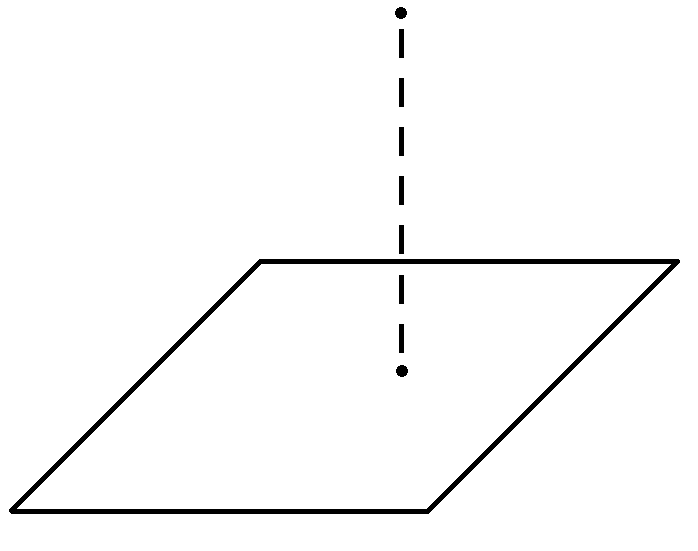
\includegraphics[width=\linewidth, height=2.0cm, right]{projection}
				\captionsetup{labelformat=empty}
				\put(-37, 60){$Y$}
				\put(-53, 40){\large $\searrow$}
				\put(-63, 50){$P$}
				\put(-35, 17){$X\hat b$}
				\put(-100, 20){$R(X)$}
		\end{minipage}
		\begin{minipage}{0.7\textwidth}
			\[R(X) = \{Xb\ | \ b \in \MR^k \} \in \MR^n \]
			её диапазон, то наивной оценкой $Xb$ является ортогональная проекция $Y$ на $R(X)$. Тогда любой вектор $\hat b$ такой, что $P(Y) = X \hat b$ является приемлемой оценкой $b$.
		\end{minipage}
	\end{center}	
\end{rmrk}

\begin{defn}
	Мы назовем $G \in \MR^{n \times m}$ \textbf{\textit{обобщенной обратной матрицей}} к матрице $A \in \MR^{m \times n}$, если
	\[ AGA = A. \]
	Зададим множество обобщенных обратных к $A$ матриц:
	\[ A^- = \{ G \ |\ AGA = A \}. \]
\end{defn}

\begin{rmrk}
	Мы будем писать $A^-$ вместо $G$, если действенность формулы не зависит то выбора обобщенной обратной матрицы. Например, $AA^-A=A$.
\end{rmrk}

\begin{exmp}
	Пусть 
	\[ A = \begin{pmatrix}
	1 & 1 \\
	1 & 1
	\end{pmatrix}. \]
	Обобщенные обратные матрицы, например:
	\[ 
	G_1 = \frac{1}{4}
	\begin{pmatrix}
	 1 & 1 \\
	 1 & 1
	\end{pmatrix}
	\quad \text{и} \quad
	G_2 = \frac{1}{2}
	\begin{pmatrix}
	1 & 0 \\
	0 & 1
	\end{pmatrix}.
	\]
\end{exmp}

\begin{lmm}[\textbf{Включение диапазона}] \label{Range inclusion}
	Пусть $X \in \MR^{n \times k}$ и $V \in \MR^{n \times s}$. Тогда:
	\begin{enumerate}
		\item $R(X) \subset R(V) \quad \Longleftrightarrow \quad VV^-X = X.$
		\item Если (i) соблюдается и $V \geq 0$ (также $n = s$), то
		\begin{enumerate}
			\item $X^T V^-X = 0,$
			\item $R(X^T) = R(X^TV^-X).$
		\end{enumerate}
	\end{enumerate}
\end{lmm}
\begin{proof}
	\begin{enumerate}
		\item Напомним, что
		\[ R(X) \subset R(V) \quad \Longleftrightarrow \quad X = VW. \]
		
		''$\Longleftarrow$'' \checkmark. \\
		''$\Longrightarrow$'' Пусть $X = VW$ и $G$ -- обобщенная обратная матрица $V$. Тогда
		\[ VGX = VGVW = VW = X. \]
		\item
		\begin{enumerate}
			\item Пусть $G$ -- обобщенная обратная матрица $V$. Тогда вследствие симметричности $V$
		    \[ X^TGX = W^TV^TGVW = W^TVW \geq 0. \]
		    \item Напомним некоторые теоремы из линейной алгебры:
		    \begin{enumerate}
		    	\item Матрица $V$ симметричная и неотрицательно определенная $\Longrightarrow$ её собственные числа $\lambda_i$ вещественные и неотрицательные
		    	$\Longrightarrow V = \sum_{i=1}^n \lambda_i z_i z_i^T$ ($z_i$ -- ортонормальные собственные вектора)
		    	$\Longrightarrow V^\alpha = \sum_{i=1}^{n} \lambda_i^\alpha z_i z_i^T$ для $\alpha \geq 0$ и $V^{\alpha + \beta} = V^\alpha V^\beta$.
		    	\item $r(A) = r(A^TA)$ и $r(A \cdot B) \leq \min{\{r(A), r(B)\}}$.
		    	В частности, $r(VW) = r(W^TVW)$, так как
		    	\[ r(VW) = r(V^{\frac{1}{2}}V^{\frac{1}{2}}W) \leq r(V^{\frac{1}{2}}W) = r(W^TVW) \leq \min \{r(W^T), r(VW) \}.   \]
		    	Используя (a), мы получаем:
		    	\[ r(X^TV^-X) = r(W^TVW) = r(VW) = r(VV^-X) = r(X). \]
		    \end{enumerate}
    	\end{enumerate}  
	\end{enumerate}
\end{proof}

\begin{thm}
	В линейной модели $Y = Xb + \varepsilon$ ортогональная проекция $Y$ на $R(X)$ и её ортогональное дополнение
	\[ R(X)^{\perp} = \{Z\ | \ Z^TX = 0 \}  \]
	задаются как
	\[P = X(X^T X)^- X^T \quad \text{и} \quad R = \mathbb{I}_n - P \]
	соответственно.
\end{thm}
\begin{proof}
	Мы докажем только для $P$. Для ортогональной проекции имеют место равенства $P^T = P$ и $P^2=P$. Во-первых,
	\[ (X^TX)(X^TX)^-X^T = VV^-X^T = X^T \]
	по Лемме \ref{Range inclusion}(i) и (ii)(b). Тогда
	\[ P^2 = X(X^TX)^-X^TX(X^TX)^-X^T = X(X^TX)^-X^T = P\]
	и $P^T = P$ следует из Леммы \ref{Range inclusion} (ii)(a).
	Наконец, $P(Y) \in R(X)$, так как $P$ вида $XA$, где $A = (X^TX)^-X^T$. Также,
	\[ P(Xb) = X(X^TX)^-X^TXb = Xb. \]
\end{proof}

\begin{rmrk} \label{rmrk8.10} \
	\begin{enumerate}
		\item Разумными оценками для $Xb$ и $\sigma^2$ являются
		\[ X\hat{b} = P(Y) = X(X^TX)^-X^TY  \]
		и
		\[ \hat{\sigma}^2 = \frac{\| Y - X\hat{b} \|_2^2}{n - r} = \frac{\| RY \|_2^2}{n - r} = \frac{Y^TRY}{n - r}, \]
		где выбор знаменателя $n-r$ будет обоснован в Следствии \ref{crlr8.13}.
		\item В общем случае, не существует единственной оценки для $b$. Однако если матрица $X^TX$ обратима ($r=r(X)=k$), то
		\[X^TX\hat{b} = X^TX(X^TX)^{-1}X^TY=X^TY  \]
		и
		\[ \hat{b} = (X^TX)^{-1}X^TY. \]
		Заметим также, что
		\[ \ME[\hat{b}] = (X^TX)^{-1}X^T\ME[Y] = (X^TX)^{-1}X^TXb = b. \]
	\end{enumerate}
\end{rmrk}

\begin{exmp}
	Пусть $Y_1, \dots, Y_n$ i.i.d. $\sim \mathcal{N}(\mu, \sigma^2)$, такие что:
	\[ Y = \begin{pmatrix}
	Y_1 \\
	\vdots \\
	Y_n
	\end{pmatrix}
	=
	 \begin{pmatrix}
	 1 \\
	 \vdots \\
	 1
	 \end{pmatrix}
	 \mu +
	  \begin{pmatrix}
	  \varepsilon_1 \\
	  \vdots \\
	  \varepsilon_n
	  \end{pmatrix}
	  = X \mu + \varepsilon,
	  	 \]
	 где $\varepsilon_1, \dots, \varepsilon_n$ i.i.d. $\sim \mathcal{N}(0, \sigma^2)$. Так как
	 \[ X^TX = (1\ \dots\ 1) \begin{pmatrix}
	 1 \\
	 \vdots \\
	 1
	 \end{pmatrix} = n, \]
	 то
	 \[ P = X(X^TX)^{-1}X^T = \frac{1}{n}\begin{pmatrix}
	 1 \\
	 \vdots \\
	 1
	 \end{pmatrix}
	 (1\ \dots\ 1).  \]
	 Таким образом,
	 \[ PY = \frac{1}{n}\begin{pmatrix}
	 1 \\
	 \vdots \\
	 1
	 \end{pmatrix}
	 \sum_{i=1}^n Y_i = \begin{pmatrix}
	 1 \\
	 \vdots \\
	 1
	 \end{pmatrix} \overline{Y}_n \]
	 является оценкой $X\mu = \begin{pmatrix}
	 1 \\
	 \vdots \\
	 1
	 \end{pmatrix} \mu$. В частности, $\overline{Y}_n$ -- оценка $\mu$. Также,
	 \[ \hat{\sigma}^2 = \frac{\| Y - X\hat{\mu} \|_2^2}{n-1} = \frac{1}{n-1} \sum_{i=1}^{n}(Y_i - \overline{Y}_n)^2. \]
\end{exmp}

\begin{lmm} \label{lmm8.12}
	Пусть $Y$ -- $n$-мерная случайная величина с математическим ожиданием $\ME[Y]=\mu$ и дисперсией $\Var(Y)=V\geq 0$. Также, пусть $A,B \in \MR^{n \times n}$. Тогда:
	\begin{enumerate}
		\item $\ME[Y^TAY]=\mu^TA\mu + \tr(AV).$
		\item Пусть моменты $Y$ до четвертого порядка совпадают с моментами нормального распределения, тогда
		\begin{enumerate}
			\item $\Cov(Y, Y^TAY)=2VA\mu,$
			\item $\Cov(Y^TAY, Y^TBY)=2 \tr(AVBV)$, если $\mu = 0$.
		\end{enumerate}
	\end{enumerate}
\end{lmm}
\begin{proof}
	Упражнение.
\end{proof}

\begin{crlr}\label{crlr8.13}
	В LMM $\ME[\hat{\sigma}^2] = \sigma^2$.
\end{crlr}
\begin{proof}
	По определению и по Лемме \ref{lmm8.12}:
	\[ \ME[\hat{\sigma}^2] = \frac{\ME[Y^TRY]}{n-r} = \frac{1}{n-r}(\mu^T R \mu + \tr(\sigma^2R)),\]
	где $\mu = Xb$. Так как $R$ -- ортогональная проекция $R(X)^\perp$, то $RXb = 0$. Следовательно,
	\[ \ME[\hat{\sigma}^2] = \sigma^2 \frac{\tr(R)}{n - r}. \]
	Любая ортогональная проекция $Q$ удовлетворяет равенству
	\[ Q = A\cdot \diag(\lambda_i) \cdot A^T.\]
	Так как $Q$ идемпотентна ($Q^2=Q$), то все собственные числа равны либо $0$, либо $1$. Число единиц совпадает с рангом $Q$. Как следствие,
	\[\tr(R) = r(R) = n - r. \]
\end{proof}

\begin{thm}[\textbf{Теорема Гаусса-Маркова}] \label{Gauss-Markov}
	Рассмотрим LMM c $r(X) = k$:
	\begin{enumerate}
		\item Оценки $\hat{b}$ и $\hat{\sigma}^2$ несмещенные и некоррелированные.
		\item Оценка $\hat{b}$ -- \textbf{\textit{лучшая линейная несмещенная оценка (BLUE)}} $b$, то есть для любого вектора $\widetilde{b}=LY$, такого что $\ME[\widetilde{b}] = b$:
		\[ \Var(\widetilde{b}) \geq \Var(\hat{b}) = \sigma^2(X^TX)^{-1}. \]
		\item Оценка $\hat{\sigma}^2$ -- \textbf{\textit{лучшая квадратичная несмещенная оценка (BQUE)}} $\sigma^2$, то есть для любого вектора $\widetilde{\sigma}^2 = Y^TAY$, такого что $\ME[\widetilde{\sigma}^2] = \sigma^2$:
		\[ \Var(\widetilde{\sigma}^2) \geq \Var(\hat{\sigma}^2).  \]
	\end{enumerate}
\end{thm}
\begin{proof} \
	\begin{enumerate}
		\item Несмещенность следует из Замечания \ref{rmrk8.10} (ii) и Следствия \ref{crlr8.13}. Также,
		\[ \Cov(\hat{b}, \hat{\sigma}^2) = \frac{1}{n-k}(X^TX)^{-1}X^T \Cov(Y, Y^TRY) \]
		и из Леммы \ref{lmm8.12} (ii) (a) следует, что
		\[\Cov(Y, Y^TRY) = 2 \sigma^2 \mathbb{I}_n R Xb = 0,\]
		так как $RXb = 0$.
		\item Если $\widetilde{b}$ несмещенная, то
		\[ \ME[\widetilde{b}] = L\ME[Y] = LXb = b \quad \forall b \in \MR^k. \]
		Следовательно, $LX = \mathbb{I}_k$. Тогда
		\[ \begin{aligned}
		0 & \leq ((X^TX)^{-1}X^T-L)((X^TX)^{-1}X^T-L)^T \\
		& = (X^TX)^{-1}-(X^TX)^{-1}X^TL^T-LX(X^TX)^{-1}+LL^T \\
		& = LL^T-(X^TX)^{-1}.
		\end{aligned}\]
		Наконец, 
		\[ \Var(\widetilde{b}) = \Var(LY) = L\Var(Y)L^T = \sigma^2 LL^T \geq \sigma^2 (X^TX)^{-1} = \Var(\hat{b}). \]
		\item Может быть доказано аналогично (ii), используя Лемму \ref{lmm8.12} (ii) (b).
	\end{enumerate}
\end{proof}

\begin{lmm} \label{lmm8.15}
	Пусть $Y \sim \mathcal{N}(0, V)$ и $A \in \MR^{p \times n}$ и $B \in \MR^{q \times n}$. Тогда
	\begin{enumerate}
		\item $AY$ и $BY$ независимы, если $AVB^T = 0$.
		\item Пусть $q = n$ и $B$ ортогональная проекция. Тогда $Y^TAY$ и $BY$ независимые, если $AVB = 0$.
	\end{enumerate}
\end{lmm}
\begin{proof}
	\begin{enumerate}
		\item Свойство нормального распределения.
		\item Как в Лемме \ref{Distribution of estimators of Normal distribution}.
	\end{enumerate}
\end{proof}

\begin{thm} \label{thm8.16}
	В LMN с $r(X)=k$ оценка $(\hat{b}, \hat{\sigma}^2)^T$ UMVU для $(b, \sigma^2)^T$ и обе оценки независимые.
\end{thm}
\begin{proof}
	Независимость следует из Леммы \ref{lmm8.15}, где $A=R$ и $B=P$. \\
	UMVU: функция плотности случайной величины $Y \sim \mathcal{N}(Xb, \sigma^2 \mathbb{I}_n)$:
	\[ f(y) = c(\sigma^2) \exp \Big \{ -\frac{1}{2\sigma^2} \| y - Xb \|_2^2  \Big \} = \widetilde{c}(\sigma^2, b) \exp \Big \{ -\frac{1}{2\sigma^2} y^Ty - 2b^TX^Ty  \Big \}.  \]
	Следовательно, мы получаем $(k+1)$-мерное экспоненциальное семейство. Статистики $Y^TY$ и $X^TY$ являются достаточными (Теорема \ref{thm4.22}) и полными (Теорема \ref{thm4.25}) для оценки $(b \sigma^2)^T$. Статистика $(\hat{b}, \hat{\sigma}^2)^T$ также достаточная и полная (Замечание \ref{rmrk4.31}). Теорема \ref{Lehmann-Scheffe} завершает доказательство.
\end{proof}

\begin{exmp}[\textbf{Метод наименьших квадратов}]
	Рассмотрим линейную регрессию:
	\[ Y_i = b_0 + b_1 X_i + \varepsilon_i.\]
	Если 
	\[X = \begin{pmatrix}
	1 & X_1 \\
	\vdots &  \vdots \\
	1 & X_n
	\end{pmatrix}\]
	-- матрица полного ранга, то $\hat{b} = (X^TX)^{-1}X^TY$. Пусть $\overline{X}_n = \frac{1}{n}\sum_{i=1}^{n}X_i$ и $\overline{X^2}_n = \frac{1}{n}\sum_{i=1}^{n}X_i^2$, тогда:
	\[ X^TX = n \begin{pmatrix}
	1 & \overline{X}_n \\
	\overline{X}_n & \overline{X^2}_n
	\end{pmatrix}. \]
	Обратная матрица
	\[ (X^TX)^{-1} = \frac{1}{\sum_{i=1}^{n}(X_i - \overline{X}_n)^2} \begin{pmatrix}
	\overline{X^2}_n & -\overline{X}_n \\
	-\overline{X}_n & 1
	\end{pmatrix}  \]
	существует, если все $X_i$ принимают различные значения. Также,
	\[ X^TY = \begin{pmatrix}
	\sum_{i=1}^{n} Y_i \\
	\sum_{i=1}^{n} X_iY_i
	\end{pmatrix}. \]
	Наконец, $\hat{b} = (\hat{b}_0, \hat{b}_1)^T$, где
	\[ \hat{b}_0  = \overline{Y}_n - \hat{b}_1\overline{X}_n, \]
	\[ \hat{b}_1 = \frac{\sum_{i=1}^{n} (X_i - \overline{X}_n)(Y_i - \overline{Y}_n) }{\sum_{i=1}^{n} (X_i - \overline{X}_n)^2} \]
	и
	\[ \hat{\sigma}^2 = \frac{1}{n-2} \sum_{i=1}^{n} (Y_i - \hat{b}_0 - \hat{b}_1 X_i )^2.  \]
\end{exmp}

\begin{rmrk}
	Часто мы заинтересованы не в $b$, но в $K^Tb$ для некоторого $K \in \MR^{k \times s}$. Если $r(X) = k$, то разумной оценкой будет:
	\[ K^T\hat{b} = K^T(X^TX)^{-1}X^TY. \]
	Даже если $r(X) \neq k$, но $R(K) \subset R(X^T)$, то оценка
	\[ K^T\hat{b} = K^T(X^TX)^{-}X^TY \]
	единственна по Лемме \ref{Range inclusion} и
	\[\ME[K^Tb] = K^T(X^TX)^-X^TXb = K^Tb. \]
\end{rmrk}

\begin{defn}
	Пусть $K \in \MR^{k \times s}$ и $r(K) = s$. Тогда мы назовем $K^Tb$ \textbf{\textit{оцениваемым}}, если $R(K) \subset R(X^T)$.
\end{defn}

\begin{exmp}
	Допустим, мы тестируем
	\[H_0: K^Tb = 0 \quad \text{против} \quad H_1: K^Tb \neq 0. \]
	Не должно быть ситуации, в которой одновременно $Xb_1 = Xb_2$ и $K^Tb_1 \neq K^Tb_2$, так как $b$ может быть получено только из $Xb$ в модели $Y = Xb + \varepsilon$. Другими словами, если мы зададим множество
	\[ N(A) = \{ y\ |\ Ay=0 \},\]
	то
	\[ Xb_1 = Xb_2 \quad \Longrightarrow \quad K^Tb_1 = K^Tb_2 \]
	эквивалетно
	\[ N(X) \subset N(K^T)\quad \Longleftrightarrow \quad R(X^T)^\perp \subset R(K)^\perp \quad \Longleftrightarrow \quad R(K) \subset R(X^T). \]
\end{exmp}

\begin{thm}
	Пусть $K^Tb$ оцениваем. Тогда:
	\begin{enumerate}
		\item В LMM $K^T\hat{b}$ -- BLUE для $K^Tb$, где
		\[ \Var(K^T\hat{b}) = K^T \sigma^2(X^TX)^{-1}K \in \MR^{s \times s}. \]
		\item В LMM $K^T\hat{b}$ -- UMVU для $K^Tb$.
	\end{enumerate}
\end{thm}
\begin{proof}
	Как в Теоремах \ref{Gauss-Markov} и \ref{thm8.16}.
\end{proof}

\begin{exmp} \
	\begin{enumerate}
		\item Рассмотрим линейную регрессию: $Y_i = b_0 + b_1x_i + \varepsilon_i$, $i = 1, \dots, n$, где $\ME[\varepsilon_i] = 0$ и $\Var(\varepsilon_i) = \sigma^2 > 0$. В векторной записи:
		\[
		\begin{pmatrix}
		Y_1 \\
		\vdots \\
		Y_n
		\end{pmatrix}
		=
		\begin{pmatrix}
		1 & X_1 \\
		\vdots & \vdots \\
		1 & X_n
		\end{pmatrix}
		\begin{pmatrix}
		b_0 \\
		b_1
		\end{pmatrix}
		+
		\begin{pmatrix}
		\varepsilon_1 \\
		\vdots \\
		\varepsilon_n
		\end{pmatrix}.
		\]
		Допустим, мы заинтересованы в гипотезах:
		\[ H_0: b_0 = 0 \quad \text{против} \quad H_1:b_0 \neq 0, \]
		тогда мы выбираем $K = \begin{pmatrix} 1 \\	0 \end{pmatrix}$ и, например,
		\[ X =	\begin{pmatrix}
		1 & 0 \\
		\vdots & \vdots \\
		1 & 0
		\end{pmatrix} . \]
		Очевидно, что $R(X) \subset R(K^T)$. Также,
		\[ X^TX =	\begin{pmatrix}
		n & 0 \\
		0 & 0
		\end{pmatrix} . \]
		не обратима, но мы можем взять
		\[ G = \frac{1}{n}	\begin{pmatrix}
		1 & 0 \\
		0 & 0
		\end{pmatrix} \]
		как обобщенную обратную матрицу и $K^T\hat{b}$ становится:
		\[ K^TGX^TY = \frac{1}{n} \sum_{i=1}^n Y_i = \overline{Y}_n. \] 
		\item Рассмотрим анализ дисперсий для $a = 3$:
		\[ Y_{ij} = \mu_i + \varepsilon_{ij} \quad (i = 1,2,3,\ j =1, \dots, n_i ). \]
		В векторной записи:
		\[
		\begin{pmatrix}
		Y_{11} \\
		\vdots \\
		Y_{1n_1} \\
		Y_{21} \\
		\vdots \\
		Y_{2n_2} \\
		Y_{31} \\
		\vdots \\
		Y_{3n_3}
		\end{pmatrix}
		=
		\begin{pmatrix}
		\mathds{1}_{n_1} & 0 & 0 \\
		0 & \mathds{1}_{n_2} & 0 \\
		0 & 0 & \mathds{1}_{n_3}
		\end{pmatrix}
		\begin{pmatrix}
		\mu_1 \\
		\mu_2 \\
		\mu_3
		\end{pmatrix}
		+
		\begin{pmatrix}
		\varepsilon_{11} \\
		\vdots \\
		\varepsilon_{1n_1} \\
		\varepsilon_{21} \\
		\vdots \\
		\varepsilon_{2n_2} \\
		\varepsilon_{31} \\
		\vdots \\
		\varepsilon_{3n_3}
		\end{pmatrix}.
		\]
		Если мы хотим проверить:
		\[H_0: \mu_1 = \mu_2 = \mu_3 \quad \text{против} \quad H_1:\mu_i \neq \mu_j \text{ для некоторых } i \neq j,\]
		то мы можем выбрать
		\[ K^T\mu = \begin{pmatrix}
		1 & -1 & 0 \\
		0 & 1 & -1
		\end{pmatrix}
		\begin{pmatrix}
		\mu_1 \\
		\mu_2 \\
		\mu_3
		\end{pmatrix}
		=
		\begin{pmatrix}
		\mu_1 - \mu_2 \\
		\mu_2 - \mu_3
		\end{pmatrix}.  \]
	\end{enumerate}
\end{exmp}

\begin{rmrk}
	Мы рассматриваем
	\begin{center}\centering
		\begin{minipage}{0.18\linewidth}
			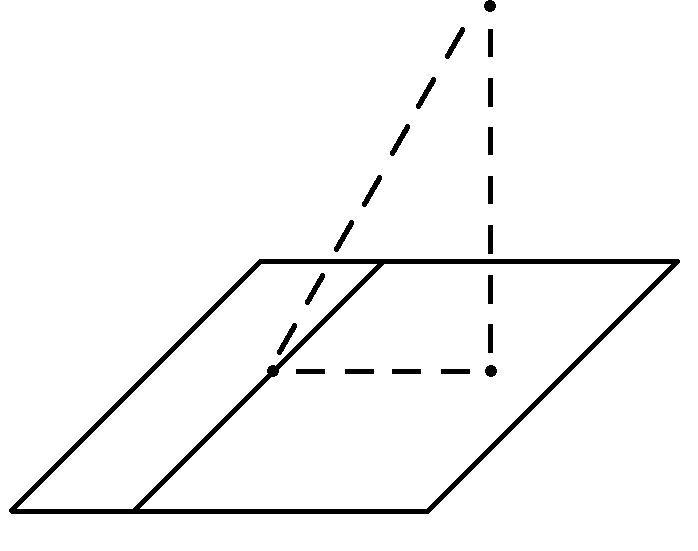
\includegraphics[width=\linewidth, height=2.0cm, right]{projection_hyp}
			\captionsetup{labelformat=empty}
			\put(-27, 60){$Y$}
			\put(-56, 41){\large $\searrow$}
			\put(-66, 53){$P_{H_0}$}
			\put(-46, 8){$P_1$}
			\put(-24, 38){$P_0$}
			\put(-98, 20){$L_{H_0}$}
			\put(-79, 11){\large $\searrow$}
			\put(-21, 5){$R(X)$}
		\end{minipage}
		\begin{minipage}{0.7\textwidth}
			\[H_0: K^Tb = 0 \quad \text{против} \quad H_1:K^Tb \neq 0, \]
			где $R(K) \subset R(X^T)$. В таком случае решающей величиной будет являться расстояние от $Y$ до пространства гипотезы:
			\[ L_{H_0} = \{ XB\ |\ K^Tb=0,\ b \in \MR^k \} \subset R(X). \]
		\end{minipage}
	\end{center}	
	Ортогональная проекция $Y$ на $L_{H_0}$: 
	\[P_{H_0} = P_0 - P_1,\]
	где
	\[ P_0 = X(X^TX)^-X^T \]
	и
	\[ P_1 = X(X^TX)^-K (K^T(X^TX)^-K)^- K^T(X^TX)^-X^T. \]
	$P_1$ также является ортогональное проекцией. При построении критерия разумно опираться на расстояние между $P_0Y$ и $P_{H_0}Y$. По теореме Пифагора:
	\[ \| (\mathbb{I}_n-P_{H_0})Y \|_2^2 - \| (\mathbb{I}_n-P_0)Y \|_2^2 =  \|P_1Y \|_2^2 = Y^TP_1Y. \]
	Последнее равенство следует из свойства идемпотентности матрицы $P_1$.
\end{rmrk}

\begin{thm}
	Пусть $Y \sim \mathcal{N}(\mu,\sigma^2 \mathbb{I}_n)$ и $P \in \MR^{n \times n}$, где $P^T=P$. Тогда $P$ -- ортогональная проекция тогда и только тогда, когда
	\[ Q = \frac{(Y - \mu)^T P (Y - \mu)}{\sigma^2} \sim \mathcal{X}_{r(P)}^2. \]
\end{thm}
\begin{proof} \\
	
	''$\Longrightarrow$'' Если $P^2 = P$, то существует $A \in \MR^{n \times n}$, где $A^TA = AA^T = \mathbb{I}_n$, такая что
	\[ A^TPA = \begin{pmatrix}
	\mathbb{I}_n & 0 \\
	0 & 0
	\end{pmatrix}, \]
	где $r = r(P)$. Мы знаем, что $Z = A^T(Y-\mu) \sim \mathcal{N}(0, \sigma^2 \mathbb{I}_n)$. Тогда
	\[ Q = \frac{(Y-\mu)^TP(Y-\mu)}{\sigma^2} = \frac{Z^TA^TPAZ}{\sigma^2} = \sum_{i=1}^{r}\Big( \frac{Z_i}{\sigma} \Big)^2 \sim \mathcal{X}_r^2.   \]
	
	''$\Longleftarrow$'' Так как $P^T=P$, существует матрица $B$, такая что $B^TB=BB^T=\mathbb{I}_n$ и
	\[ B^TPB = \Lambda = \diag(\lambda_1, \dots, \lambda_n),  \]
	где $\lambda_i$ -- вещественнозначные собственные числа $P$. Подставляя $X = B^T(Y-\mu) \sim \mathcal{N}(0, \sigma^2 \mathbb{I}_n )$, получаем
	\[ Q = \frac{1}{\sigma^2} X^TB^TPBX. \]
	Так как $Q \sim \mathcal{X}_r^2$, то её характеристическая функция:
	\[ \ME[\exp\{itQ\}] = (1-2it)^{-r/2}, \]
	и также:
	\[ \begin{aligned}
	\ME[\exp\{itQ\}] & = \ME \Big[ \exp\Big\{ \frac{it}{\sigma^2} X^TB^TPBX \Big\}\Big] = \ME \Big[ \exp\Big\{ it \sum_{j=1}^n \lambda_j \Big( \frac{X_j}{\sigma} \Big)^2 \Big\}\Big] \\
	& = \prod_{j=1}^{n} \ME \Big[ \exp\Big\{it \lambda_j \Big( \frac{X_j}{\sigma} \Big)^2 \Big \}\Big] = \prod_{j=1}^{n} (1 - 2it\lambda_j).
	\end{aligned} \]
	Поскольку полином однозначно определяется его линейными множителями, $\lambda_1 = \dots = \lambda_r = 1$ и $\lambda_j = 0 \ \forall j > r$. В частности,
	\[ P^2 = B\Lambda B^T B\Lambda B^T = B^T \Lambda^2 B^T= B\Lambda B^T = P. \]
\end{proof}

\begin{rmrk} \label{rmrk8.25}
	Пусть $Y \sim \mathcal{N}(\mu,\sigma^2 \mathbb{I}_n)$ и $P$ -- ортогональная проекция, где $r(P) = r$. Задав
	\[ A^TPA = \begin{pmatrix}
	\mathds{1}_r & 0 \\
	0 & 0
	\end{pmatrix},  \]
	мы получаем
	\[\widetilde{Q} = \frac{Y^TPY}{\sigma^2} = \frac{\widetilde{Z}^TA^TPA\widetilde{Z}}{\sigma^2},\]
	где
	\[ \widetilde{Z} = A^TY \sim \mathcal{N}(A^T\mu, \sigma^2\mathds{1}_n). \]
	Можно показать, что распределение
	\[ \widetilde{Q} = \sum_{i=1}^r \Big( \frac{\widetilde{Z}_i}{\sigma} \Big)^2  \]
	зависит только от $r$ и
	\[ \delta^2 = \sum_{i=1}^r \Big( \frac{(A^T\mu)_i}{\sigma} \Big)^2 = \frac{\mu^T P \mu}{\sigma^2}. \]
	Оно называется смещенным распределением $\mathcal{X}^2$ с $r$ степенями свободы и смещением $\delta^2$. Обозначение: $\widetilde{Q} \sim \mathcal{X}_{r, \delta^2}^2$.
\end{rmrk}

\begin{defn}
	Пусть $X \sim \mathcal{X}_m^2$ и $Y \sim \mathcal{X}_n^2$ независимы. 
	\begin{enumerate}
		\item Распределение случайной величины
		\[ F = \frac{nX}{mY} \]
		называется \textbf{\textit{F-распределением с $m$ и $n$ степенями свободы}}. Обозначение $F \sim F_{m,n}$.
		\item Если $X \sim \mathcal{X}_{m, \sigma^2}^2$, то
		\[ F = \frac{nX}{mY} \sim F_{m,n,\sigma^2}. \]
	\end{enumerate}
\end{defn}

\begin{thm}[\textbf{F-критерий в LMN}]
	В LMN пусть $R(K) \subset R(X^T)$, $t = r(K)$ и $r = r(X)$. Тогда
	\begin{enumerate}
		\item  \[ F = \frac{\frac{1}{t}\|P_1Y \|_2^2}{\frac{1}{n-r}\| RY \|_2^2} \sim F_{t, n-r, \delta^2}, \]
		где 
		\[\delta^2 = \frac{1}{\sigma^2} (K^Tb)^T(K^T(X^TX)^-K)^-K^Tb \]
	    и
	    \[ R = \mathbb{I} - P_0 \]
	    как прежде.
	    \item
	    \[ \varphi(Y) =
	    \left \{
	    \begin{array}{cl}
	    1, &  F >  F_{t, n-r, 1-\alpha}\\
	    0, & \text{иначе}. 
	    \end{array}
	    \right.
	    \]
	    -- \textbf{\textit{F-критерий}} для
	    \[ H_0: K^Tb = 0 \quad \text{против} \quad H_1: K^Tb \neq 0  \]
	    с уровнем значимости $\alpha$.
	\end{enumerate}
\end{thm}
\begin{proof}
	Достаточно показать (i). Из Замечания \ref{rmrk8.25} следует:
	\[ \frac{\| P_1Y \|_2^2}{\sigma^2} = \frac{Y^TP_1Y}{\sigma^2} \sim \mathcal{X}_{t, \delta^2}^2 \]
	и
	\[ \delta^2 = \frac{(Xb)^TP_1Xb}{\sigma^2} = \frac{(K^Tb)^T (K^T(X^TX)^-K)^-K^Tb}{\sigma^2}, \]
	исходя из определения $P_1$. Аналогично $\frac{Y^TRY}{\sigma^2} \sim \mathcal{X}_{n-r}$, так как $RXb = 0$. Лемма \ref{lmm8.15} и $P_1R=0$ завершают доказательство.
\end{proof}

\backmatter

% bibliography, glossary and index would go here.
\addcontentsline{toc}{chapter}{Список литературы}
\bibliographystyle{stylefile}
\bibliography{biblio}

\end{document}